\chapter{Experimental Apparatus}

\section{Introduction}

There are several major components of our experimental apparatus: the laser system, the vacuum system, the XUV-IR optics and interferometer, the target chamber and the XUV detector. Many of these subsystems were designed as improvements upon previously available equipment in the DiMauro lab, so comparisons will be made when applicable.

The laser system is the linchpin of our experiment. Its short mid-infrared pulse allows us generate XUV light via an extremely nonlinear process, photoexcite the sample and ultimately probe ultrafast dynamics in the samples. The pointing, power, and pulse duration stability of the laser system enables us to perform these sensitive experiments over extended periods of time. Details of the laser system and the general laboratory layout are discussed in \cref{sec:Laser_System}.

XUV light cannot propagate in air. Therefore, much of the experiment is performed under high vacuum using a home-built vacuum apparatus, as shown in \cref{fig:TABLE_overhead_drawing,fig:TABLE_angled_drawing}. Details of the vacuum system are discussed in \cref{sec:Vacuum_System}.

After high harmonic generation, the XUV light needs to be spatially and spectrally manipulated before it can be used in our experiment. Most materials absorb strongly in this energy range, so special XUV optics are used for this purpose. Details of the XUV optics, along with a description of the XUV-IR interferometer, are discussed in \cref{sec:Interferometer_Design}. 

The XUV light is focused on our sample in a target chamber, and the transmitted light is detected by a home-built XUV photon spectrometer. A brief overview of these systems can be found in \cref{sec:XUV_spectrometer}. A detailed description of these subsystems can be found in Stephen Hageman's dissertation \cite{hagemanComplexAttosecondTransientAbsorption2020}.


\section{Laser System}
\label{sec:Laser_System}

\subsection{Spitfire and TOPAS}

We use a commercial mid-IR laser system (Spectra Physics Spitfire ACE), which delivers 12 mJ of 800 nm light at a variable $100 - 1,000$ Hz repetition rate with a 60 fs FWHM pulse duration. This system utilizes the chirped pulse amplification (CPA) technique to amplify the pulse energy from a weak seed pulse. In this scheme, a low energy femtosecond seed pulse is stretched in time, amplified and compressed \cite{stricklandCompressionAmplifiedChirped1985}. As such, the Spitfire consists of an oscillator, a grating stretcher, a regenerative amplifier, a single-pass amplifier and a grating compressor.

\begin{figure}
	\centering
	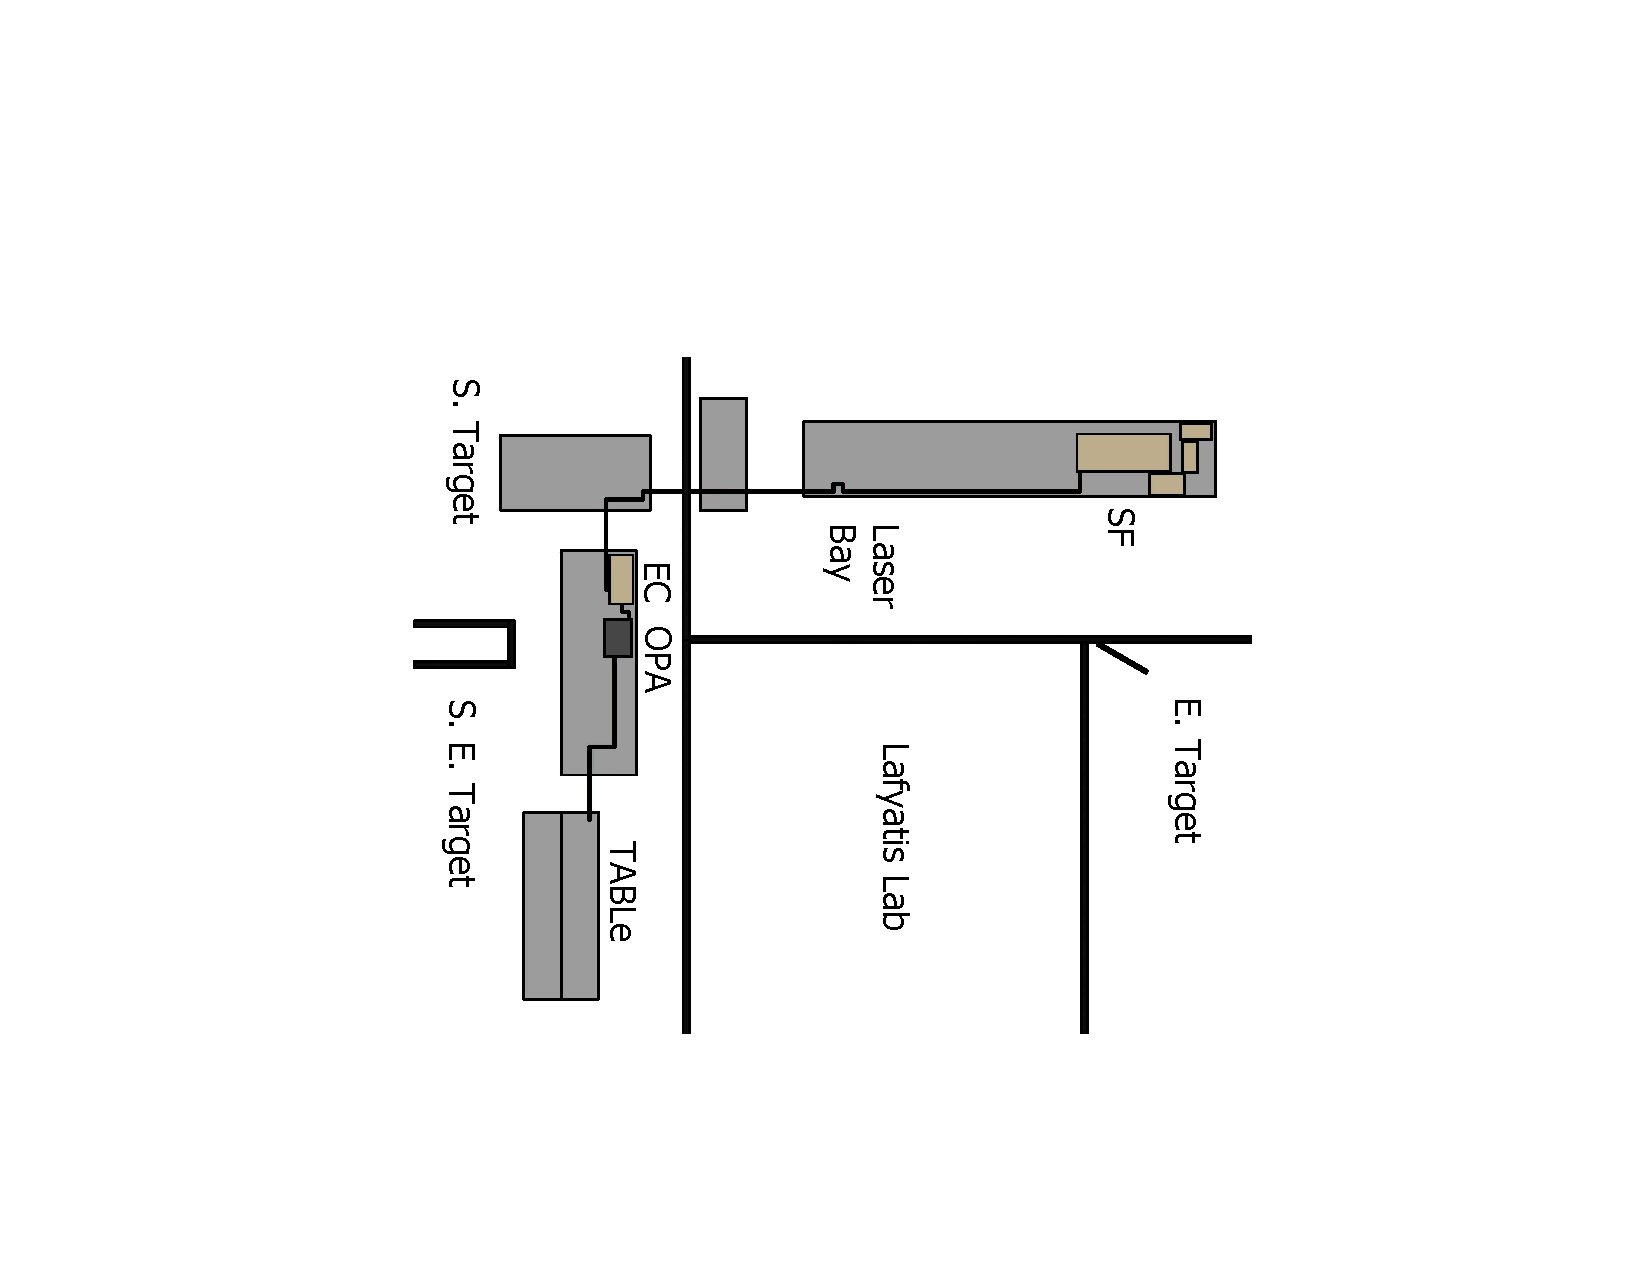
\includegraphics[width=0.95\textwidth,angle=90]{figures/chap2/beam_routing2.pdf}
	\caption{Block diagram of part of the DiMauro lab complex showing the laser path from the laser bay to the southeast target room. Other experiments and laser systems are ommitted for visual clarity. Optical tables are represented as gray boxes. SF: Spitfire laser system consisting of a MaiTai oscillator, two Empower pump lasers, interal stretcher, amplifier \& internal compressor (bypassed for this experiment); EC: Spitfire external compressor; OPA: Light Conversion HE TOPAS Prime; TABLe: $4' \times 10'$ optical table for the transient absorption beamline.}
	\label{fig:beam_routing}
\end{figure}

The laboratory layout is shown in \cref{fig:beam_routing}. All of the lasers in the DiMauro research group are located in a centralized laser bay, where foot traffic is kept to a minimum and air quality is nominally higher than the surrounding laboratory areas. This minimizes air disturbances around the laser systems and reduces the accumulation of dirt and debris on their optics. Experiments are performed in the adjacent target rooms which contain the vacuum systems and other experimental equipment. The Spitfire shares the laser bay with two home-built ultrafast laser systems (the ``2 micron system'' and the ``4 micron system'', not shown in \cref{fig:beam_routing}), as well as some laser development. The Spitfire is positioned so that its light can be directed to either the East, South or Southeast Target Rooms, depending on the needs of the researchers. To reduce air currents, welding curtains surround each optical table in the laser bay. When propagating the beam to target rooms, the beam path is enclosed in PVC tubing to reduce air currents and to increase user safety. A CaF\textsubscript{2} window is used to block air currents between the laser bay and the target rooms.

Referring to \cref{fig:beam_routing}, the transient absorption beamline (TABLe) is located in the southeast target room. Laser light from the amplifier must be propagated uncompressed to the target room to avoid nonlinear propagation effects. To understand why we can compute the $B$ integral, which provides a measure of the nonlinear phase accumulated during propagation: 

\begin{equation}
B = \frac{2 \pi}{\lambda} \int n_2 I(z) \dd{z}
\label{eqn:B-integral}
\end{equation}
%this calculation was done in B-integral.nb mathematica notebook

The distance between the amplifier and the south target room is approximately 13 meters. For a propagation distance of 13 meters, a beam radius of 0.8 cm, a pulse energy of 12 mJ and a FWHM pulse duration of 60 fs, $B = 1.53$, which indicates that nonlinear propagation effects are significant \cite{zahedpourMeasurementNonlinearRefractive2015}. On the other hand, the uncompressed pulse has slightly higher pulse energy (15 mJ, owing to the 20\% transmission losses of the compressor), but a significantly longer pulse duration ($\sim 10^3$ longer), resulting in a negligible $B$ value. For this reason, we use an external compressor centrally located between the south and south east target rooms, as shown in \cref{fig:beam_routing}. This positioning allows the Spitfire to be used for either the TABLe in the southeast target room or the RABBITT apparatus \cite{chirlaAttosecondPulseGeneration2011,gormanAttosecondProbingElectron2018,kiesewetterDynamicsNearThresholdAttosecond2019} in the south target room (not shown in \cref{fig:beam_routing}). The external compressor has an efficiency of 80\%, giving us 12 mJ of 800 nm light with a FWHM pulse duration of 60 fs at the entrance of the OPA.

The output of the external compressor is sent into a commercial optical parametric amplifier (Light Conversion HE TOPAS Prime), which converts the 800 nm light to longer wavelengths ranging from 1.2 to 2.2 $\mu$m while roughly maintaining pulse duration. To minimize nonlinear propagation effects, the TOPAS is located immediately after the external compressor with only two steering mirrors between the external compressor and the TOPAS. Details of the TOPAS operation, alignment and optimization can be found in the user manual. Briefly, it utilizes a nonlinear process called optical parametric amplification (OPA), where the 800 nm pump ($p$) is converted into two longer wavelength photons (the signal $s$ and the idler $i$) that obey the following energy conservation relation:

\begin{equation}
\frac{1}{\lambda_p} = \frac{1}{\lambda_s} + \frac{1}{\lambda_i}
\end{equation}

Inside the TOPAS, a white light generation process creates a broadband seed pulse, followed by three stages of amplification in BBO crystals. The signal $\lambda_s$ and idler $\lambda_i$ wavelengths are determined by phase matching conditions inside the nonlinear crystals, which is controlled by setting the crystal angle relative to the incident laser light. The BBO crystals are mounted on encoded motorized stages, and the entire system is computer controlled and calibrated so the crystal angles change when the user specifies the desired wavelength. The conversion efficiency of the TOPAS ranges from 40 to 50 \% (combined signal + idler pulse energy of 5 - 6 mJ), depending on the degree of optical alignment into the TOPAS and the desired wavelength. During the amplification process, all three beams are collinear. After the final amplification stage, a dichroic mirror inside the TOPAS separates the depleted 800 nm pump from the signal + idler, and a wavelength separator immediately outside the TOPAS splits the signal from the idler.

\begin{figure}
	\centering
	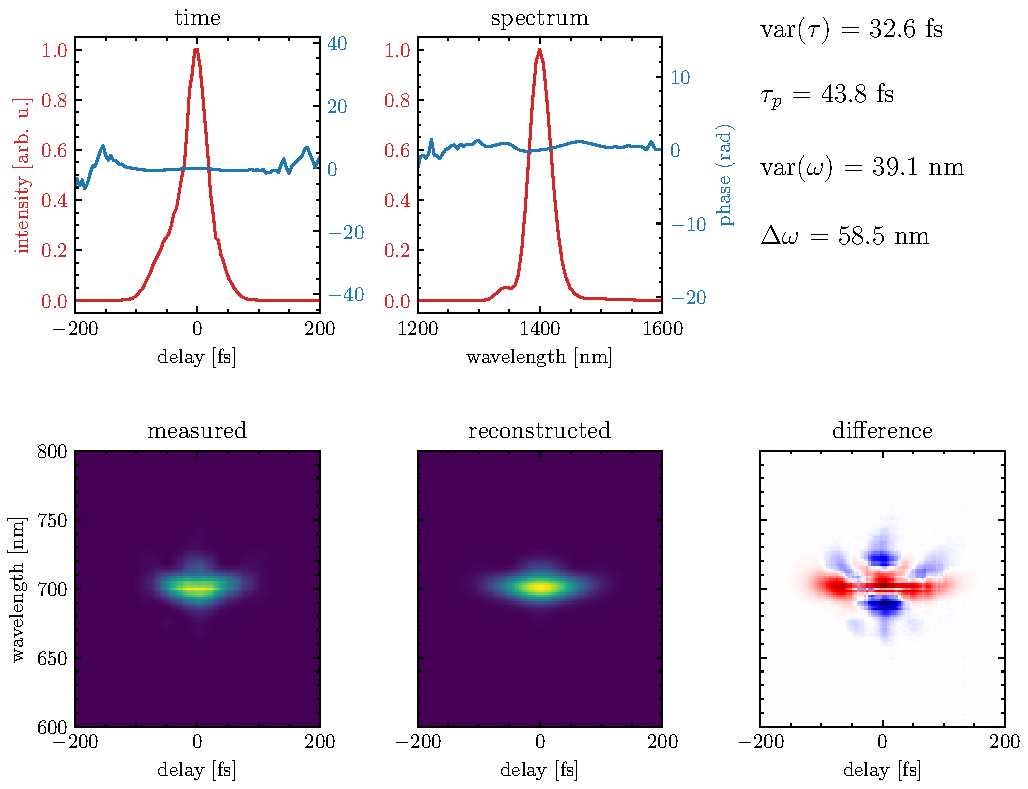
\includegraphics[width=0.75\textwidth]{figures/chap2/TOPAS_FROG_1400nm.pdf}
	\caption{FROG analysis of the signal output of the TOPAS ($\lambda = 1400 \ \textrm{nm}$).}
	\label{fig:TOPAS_FROG_1400nm}
	% figure created in \Python Scripts\FROG\FROG2.py
	% data: autosave_07_23_19_15_45_11
\end{figure}

We use the \textit{frequency resolved optical gating} (FROG) technique to measure the pulse duration of the TOPAS \cite{kaneCharacterizationArbitraryFemtosecond1993}. The result is shown in \cref{fig:TOPAS_FROG_1400nm}. At 1400 nm, we measure a pulse width (defined via the intensity FWHM) of $\tau_p = 43.8 \ \textrm{fs}$ and a pulse bandwidth (defined as the spectral intensity FWHM) of $\Delta \omega = 58.5 \ \textrm{nm}$.

The interaction pulse duration used in experiments is longer than this measured quantity, as several chromatic optics in each arm of the interferometer add GDD to the pulse. In the generation arm, there are 3 lenses and a CaF\textsubscript{2} window. In the pump arm, the pulse travels through the delay wedges (approximately 2 mm of fused silica), two BK-7 lenses (7 mm total thickness), and a 3 mm thick CaF\textsubscript{2} vacuum window. Assuming a transform-limited pulse, if the initial pulse duration is $\tau_0$, then the group delay dispersion (GDD) of these optics increases the pulse duration to $\tau$ \cite{dielsUltrashortLaserPulse2006}:
\begin{equation}
\tau = \tau_0 \sqrt{1 + \left(4 \ln 2 \frac{GDD}{\tau_0^2}\right)^2} \approx 4 \ln 2 \frac{GDD}{\tau_0}
\label{eqn:pulse_broadening}
\end{equation}
For the pump arm, \cref{eqn:pulse_broadening} evaluates to $\tau = 63.7 \ \textrm{fs}$ for an initial pulse duration of $\tau_0 = 43.8 \ \textrm{fs}$. The pulse duration of the generation interaction region is similar.

\subsection{Active Pointing Correction Systems}

As a nonlinear device, the performance of the TOPAS is extremely sensitive to input pointing, laser pulse parameters and laboratory environmental conditions. The large optical path length ($\approx 15.5$ m) between the amplifier and the TOPAS puts stringent requirements on the angular tolerances of the amplifier's output pointing. According to the specification sheet, the rms beam pointing stability of the amplifier at constant temperature is $<5\text{ } \mu \text{rad}$ ($\approx 75 \text{ } \mu \text{m}$ at 15.5 m) at constant temperature, which is sufficient for our purposes. Unfortunately, the temperature in the laser bay varies significantly throughout the day -- sometimes by several degrees -- as a function of the occupancy of the physics research building, building-wide energy conservation measures, and activity within the laser bay. Under these conditions, the amplifier's pointing changes by up to 20 $\mu \text{rad} / ^{\circ} \text{C}$ ($= 310 \text{ } \mu \text{m}/ ^{\circ} \text{C}$ at 15.5 m).

\begin{figure}
	\centering
	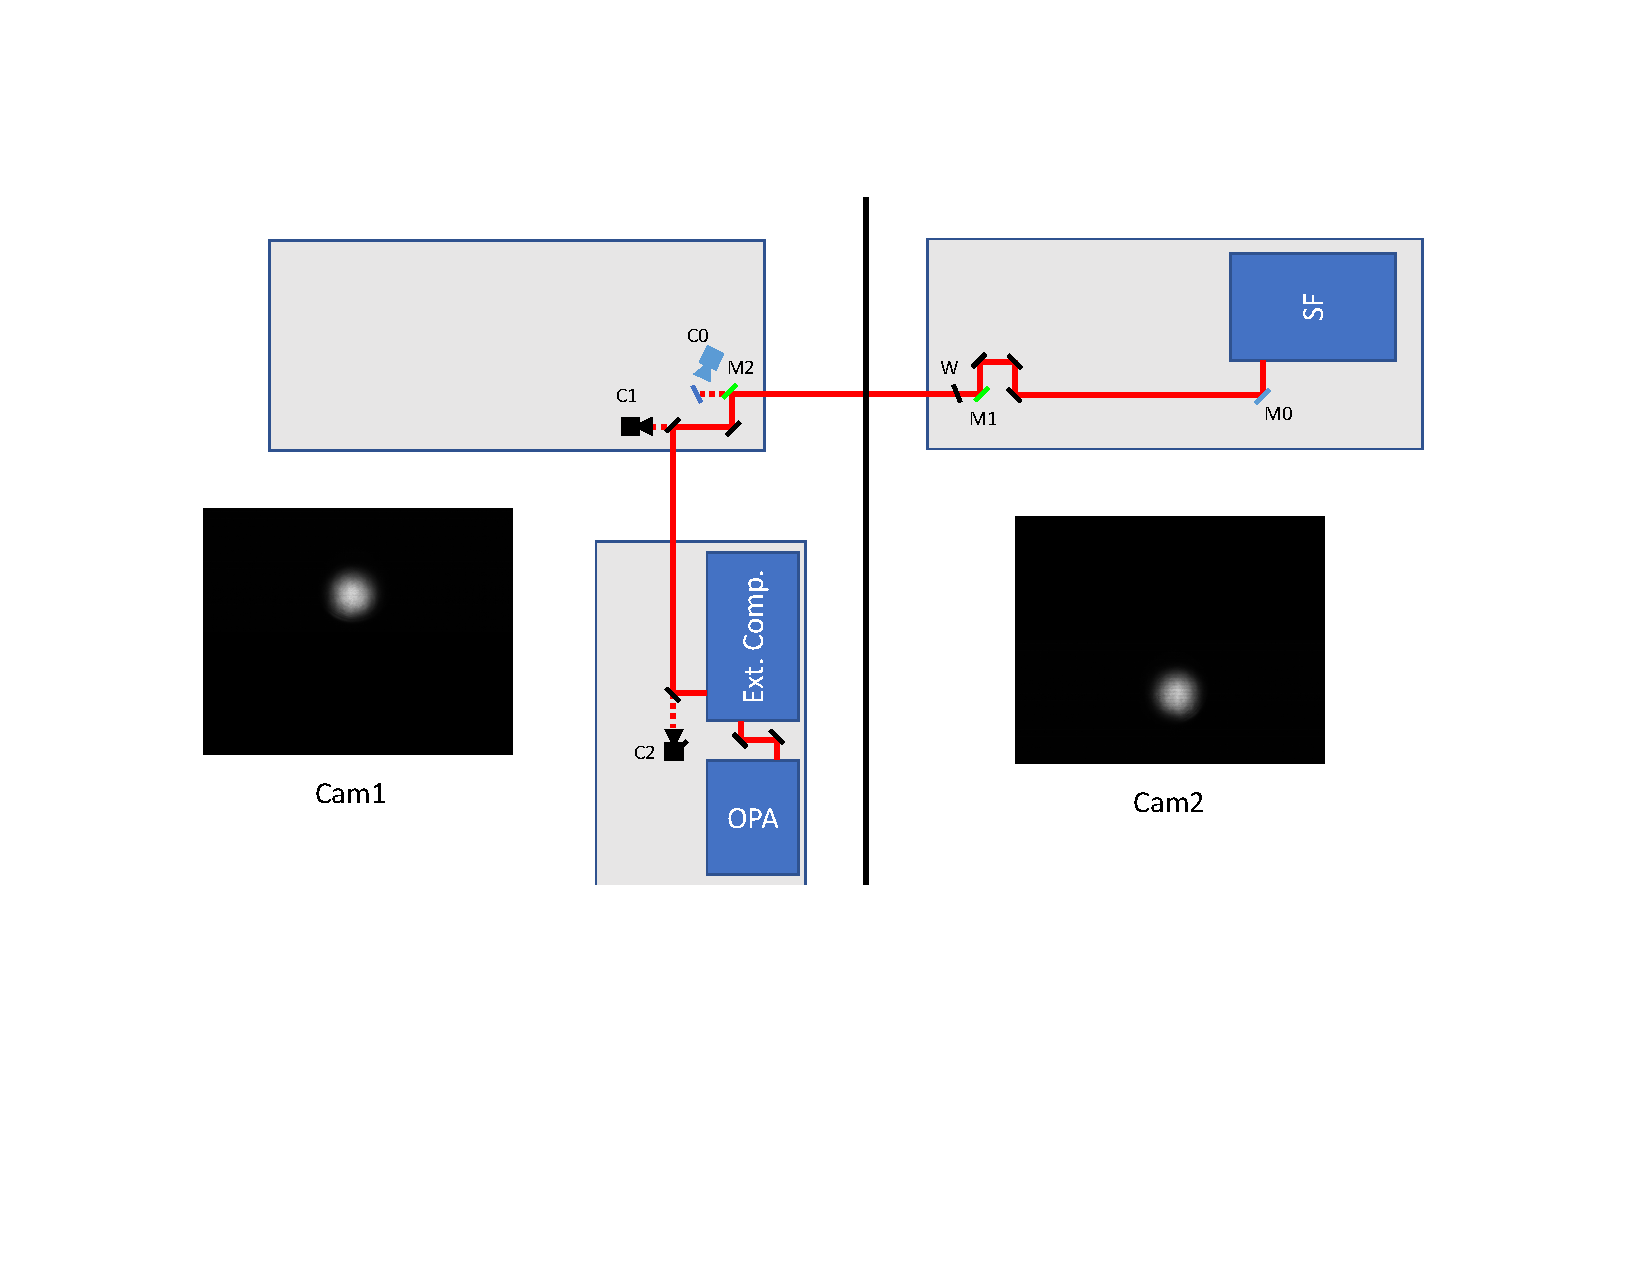
\includegraphics[width=0.75\textwidth]{figures/chap2/guidestar_geometry.pdf}
	\caption{Implementation of active stabilization systems between the amplifier in the laser bay and external compressor in the target room (not to scale). M0 \& C0 are the motorized mirror and digital camera used for the single-point correction scheme. M1, M2, C1 \& C2 are the motorized mirrors and cameras used for the two-point correction scheme. W is an uncoated CaF\textsubscript{2} window used to reduce air currents between the laser bay and target rooms. PVC tubes that surround the beam path are omitted for visual clarity. Inset images show the attenuated beam as imaged by C1 \& C2.}
	\label{fig:guidestar_geometry}
\end{figure}

To combat this slow pointing drift, we actively stabilize the beam pointing between the amplifier and the external compressor as shown in \cref{fig:guidestar_geometry}. Note that there is not enough space to implement a pointing solution between the external compressor and the TOPAS. Over the years, we have used both a home-built single-point correction scheme and a commercial two-point correction scheme.

\begin{figure}
	\centering
	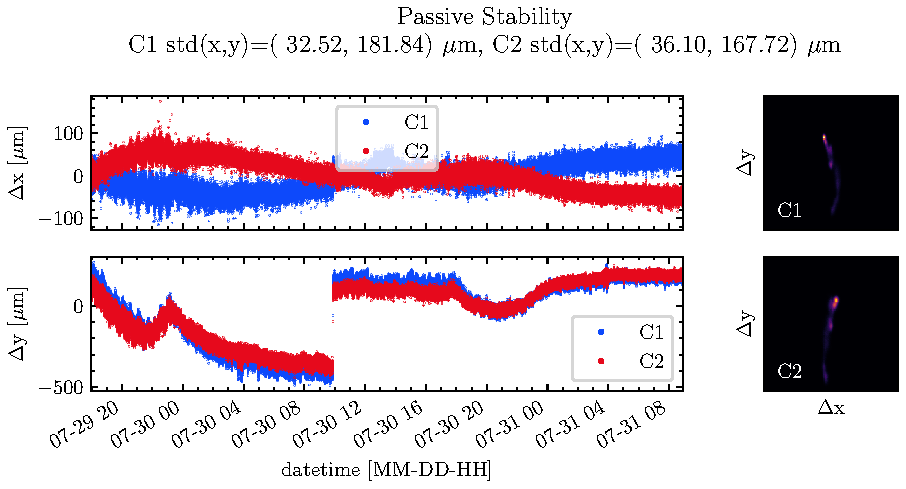
\includegraphics[width=0.75\textwidth]{figures/chap2/Stability_NoCorrection.pdf}
	\caption{Typical passive pointing stability of the Spitfire's amplifier as measured on cameras C1 \& C2. Left panels: $x$ and $y$ coordinates of the centroid vs. time; right panels: 2D histogram of beam centroid positions for the same time period. The 2-point correction scheme was activated between 09:00 (9 am) and 17:00 (5 pm) on 07-30; this system is responsible for the stable performance in the middle in the plot. Long term thermal drift is apparent at all other times.}
	\label{fig:guidestar_passive_stability}
	% dataset: 2019-07-31_8.55am_pointing.txt
	% python file: \Python Scripts\BeamTracker\dissertation_plots.py
\end{figure}

\cref{fig:guidestar_passive_stability} shows the passive pointing stability of the amplifier as measured by cameras C1 \& C2 over the course of 28 hours. The left panel shows the $x$ and $y$ coordinates of the centroid (expressed as a deviation from the average position) sampled at 2 Hz. Note that the sign of $\Delta x$ is reversed between C1 and C2; this is an artifact of the camera geometry; otherwise the data from the two cameras is self-consistent. The thermal drift is most apparent in the vertical direction; from midnight to 9 am the beam drifts vertically nearly 500 $\mu$m. Between 9 am and 5 pm we activated the two-point stabilization system (described below), which accounts for the good performance during this time period. At 5 pm, the stabilization system was turned off and the slow drift resumes. The right panels show 2D histograms of the centroid position, calculated from the time series data. From these plots, it is apparent that the laser drifts in a large arc pattern, with the primary deviation occuring in the vertical direction.

The single-point correction system was programmed and implemented by Dietrich Kiesewetter, who was a graduate student at the time \cite{kiesewetterDynamicsNearThresholdAttosecond2019}. In this scheme, a digital camera (C0 in \cref{fig:guidestar_geometry}) located approximately 7.8 m after the amplifier monitors the transmitted light of a high reflective mirror incident on a card. The position of the centroid is calculated on a rolling average basis and compared to a saved set point. When the centroid position deviates from the set point by more than a minimum correction size, a correction signal is sent to a motorized mirror (M0, located 33 cm after the amplifier). The minimum correction size is set by the user to avoid frequent small corrections to the beam, which results in high-frequency pointing jitter. The correction time interval is also user-adjustable, with typical values of 1 - 60 seconds. If the correction signal requires too large of a step, or if the integrated intensity of the beam falls below a set value, then the locking algorithm assumes that something is wrong and breaks the correction loop without taking corrective action. This prevents the system from taking corrective action in the event the beam is partially blocked by a third party.

\begin{figure}
	\centering
	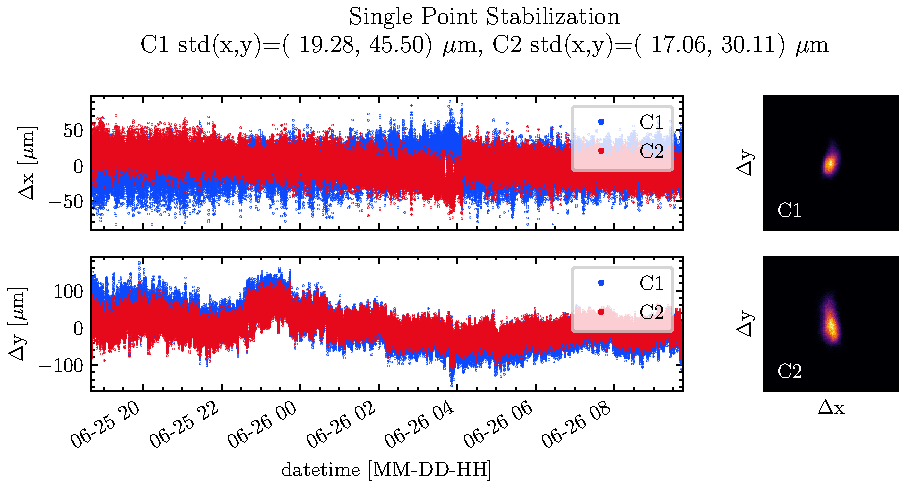
\includegraphics[width=0.75\textwidth]{figures/chap2/Stability_Dietrich_ON.pdf}
	\caption{Single-point stabilization of the Spitfire's amplifier as measured on cameras C1 \& C2. This dataset contains about 10 correction events, which are visible as abrupt jumps in the time series. The skew of the centroid distributions highlights the limitations of the single-point correction scheme.}
	\label{fig:guidestar_1point_stability}
	% dataset: 2019-06-26_09.45am_pointing.txt
	% python file: \Python Scripts\BeamTracker\dissertation_plots.py
\end{figure}

The performance of the single-point stabilization system as reported by cameras C1 \& C2 is shown in \cref{fig:guidestar_1point_stability}. Here, we can see the limitations of a single-point correction scheme. The system is very good at maintaining the position of the beam at C0, but it has no control over the pointing of the beam. As a result, the beam centroid continues to drift on downstream optics, albeit with reduced magnitude compared to the uncorrected case. This is effect is apparent in the skewed 2D histograms in \cref{fig:guidestar_1point_stability}. The single-point stabilization system works well over short periods of time, but its geometry neccessitates weekly realignment of the external compressor and all other downstream optics. Given the technical demands of our experiments and the sensitivity of the TOPAS to input pointing, this can be a prohibitively time consuming process. Unlike a single-point correction system, a two-point system only needs to be set once.

For the two-point stabilization system, a commercial system was chosen over a home-built solution to reduce the development and implementation time. We use a Newport GuideStar II, which utilizes two cameras (C1 \& C2 in \cref{fig:guidestar_geometry}) and two motorized mirrors (M1 \& M2) to monitor the beam centroid and make corrections. A patented correction algorithm running on purpose-built computational hardware is applied to the output of the cameras to solve for the neccessary correction signals up to 3 times per second \cite{farinasOpticalBeamSteering2009}. Beam pointing is usually recovered with a single corrective action, and even especially large pointing drifts are corrected well within 1 second. For numerical stability and increased sensitivity, the distance between M1 and M2 is made as large as possible (3.1 meters); the distance between C1 and C2 (1.75 meters) is also maximized and made similiar to the M1-M2 distance; the distance between C1 and M2 is made as small as possible (75 cm).

\begin{figure}
	\centering
	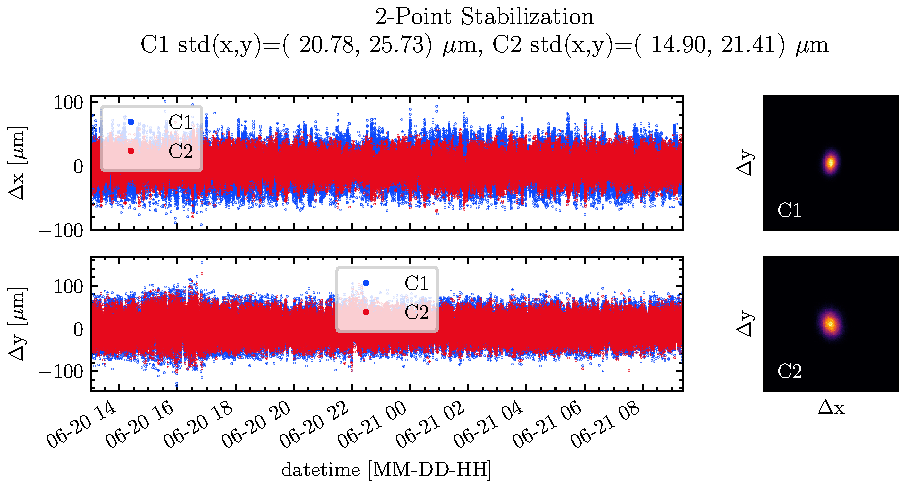
\includegraphics[width=0.75\textwidth]{figures/chap2/Stability_GuideStarII_ON.pdf}
	\caption{Two-point stabilization of the Spitfire's amplifier as measured on cameras C1 \& C2.}
	\label{fig:guidestar_2point_stability}
	% dataset: 2019-06-21_09.23am_pointing.txt
	% python file: \Python Scripts\BeamTracker\dissertation_plots.py
\end{figure}

The passive and actively-controlled pointing stability of the amplifier is shown in \cref{fig:guidestar_2point_stability}. Owing to the high correction frequency, individual corrections are small and not visible in the time series. The two-point system maintains both the centroid position and propagation direction, so there is minimal correlation between the reported centroid positions on C1 \& C2. As a result, the pointing into the TOPAS rarely needs to be optimized under normal operation, saving valuable time and making experiments more repeatable.

The GuideStar II performs extremely well, but its software lacks the safety features of our home-built system. Specifically, there is no maximum allowable correction size, intensity or beam mode quality monitoring to prevent run-away corrections. For example, it is common to insert a paper card into the beam path to inspect the beam mode just before the external compressor. As a result, camera C2 will briefly see a partially clipped beam with a centroid displaced by approximately the beam radius, and the GuideStar will take \textit{immediate corrective actions} to adjust the pointing. These actions may result in a 15 mJ beam pointing in an unsafe direction. \textbf{Users are cautioned to keep clear of the beam path between the amplifier and the GuideStar cameras when the GuideStar locking algorithm is enabled.} To mitigate this issue, the GuideStar cameras are kept in a plastic enclosure and colleagues are made aware of the limitations of the GuideStar system.

%\textbf{say something about the 2photon photodiode in the external compressor}

\subsection{Beam routing into the TABLe interferometer}

After selecting the wavelength (signal, idler or depleted pump), the output of the TOPAS is sent approximately 3 meters downsteam to the transient absorption optical table. Two motorized mirrors on the TOPAS optical table are used to align the laser into the TABLe interferometer. Unless otherwise noted, protected silver mirrors are used to propagate the TOPAS light for their broadband reflectivity, low absorption losses and high corrosion resistance. 

\section{Vacuum System}
\label{sec:Vacuum_System}
\subsection{The Need for High Vacuum}

%\begin{figure}
%	\centering
%	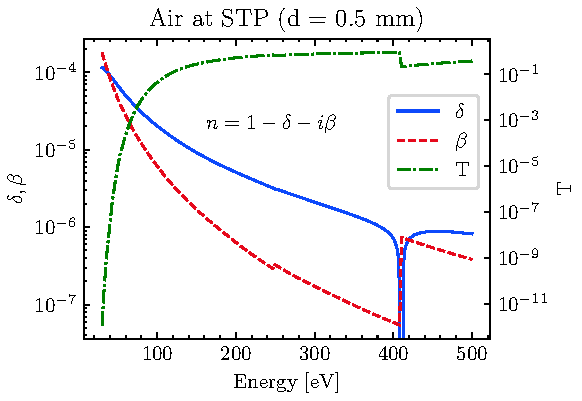
\includegraphics[width=0.75\textwidth]{figures/chap2/AirAbs.pdf}
%	\caption{Estimation of XUV propagation losses through 0.5 mm of air at STP. Atomic scattering data obtained from \cite{gulliksonCXROXRayInteractions,henkeXRayInteractionsPhotoabsorption1993}. Calculation follows \cref{eqn:PhotoCrossSection,eqn:BeersLaw,eqn:IndexfromASF}.}
%	\label{fig:AirAbs}
%	% generated using CXRO.py
%\end{figure}

The XUV light generated by the high harmonic process is absorbed strongly by air, as most gases have at least one electronic transition in the XUV regime. The magnitude of absorption can be estimated using the atomic scattering factors $f = f_1 + i f_2$, which were taken from \cite{henkeXRayInteractionsPhotoabsorption1993}. The photoabsorption cross section $\mu_a$, the transmission ratio $T$, and the complex index of refraction $\hat{n}$ of a gas can be calculated from these factors:
\begin{align}
\mu_a &= 2 r_0 \lambda f_2 \label{eqn:PhotoCrossSection} \\
T &= \exp\left( -N \mu_a d \right) \label{eqn:BeersLaw} \\
\hat{n} &= 1 - \frac{1}{2 \pi} N r_0 \lambda^2 \left(f_1 + i f_2\right) \label{eqn:IndexfromASF}
\end{align}
In the above, $\lambda$ is the photon wavelength, $N$ is the number of atoms per unit volume, $d$ is the optical path length and $r_0=2.8179403227(19) \times 10^{-6} \text{ nm}$ is the classical electron radius. Since XUV light is ionizing radiation, propagating in air at ambient pressure will cause the light to be effectively attenuated to zero in a few hundred microns. For this reason, any aspect of the experiment involving XUV light must be kept under high vacuum.

%The results for air at standard temperature and pressure are shown in \cref{fig:AirAbs}. From this figure it is apparent that any XUV light we generate will be effectively attenuated to zero in less than 1 millimeter if the beam is propagated in air.

\begin{figure}
	\centering
	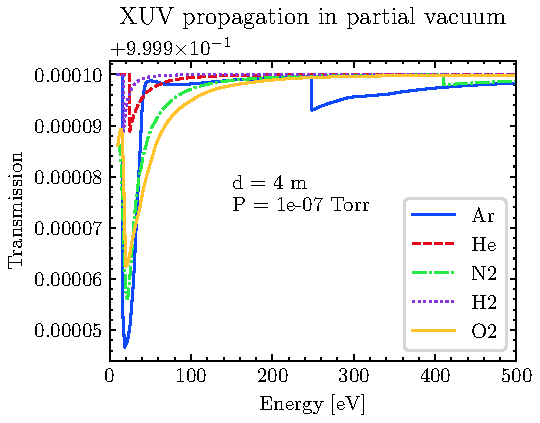
\includegraphics[width=0.75\textwidth]{figures/chap2/XUVinVacuum.pdf}
	\caption{Estimation of XUV propagation losses through a vacuum level of $10^{-7}$ Torr and a distance of 4 meters. Transmission is well over 99.999\% for this pressure-length product. Atomic scattering data obtained from \cite{gulliksonCXROXRayInteractions,henkeXRayInteractionsPhotoabsorption1993}. Calculation follows \cref{eqn:PhotoCrossSection,eqn:BeersLaw,eqn:IndexfromASF}.}
	\label{fig:XUVinVacuum}
	% generated using CXRO.py
\end{figure}

For reference, the XUV portion of the transient absorption beamline is about 4 meters long. \cref{fig:XUVinVacuum} shows the expected XUV transmission losses for XUV propagation through a partial vacuum of common gases: argon and helium are often used for generation, while nitrogen, hydrogen and oxygen are common UHV system contaminants. From this figure, we can see that the XUV transmission exceeds 99.99\% for an average pressure of $10^{-7}$ Torr. Note that this calculation does not include reflection losses from the ellipsoidal mirror, transmission losses from the metallic filter or the sample, or geometric losses from clipping. This simple analysis tells us that the XUV portion of the beamline must be kept under relatively high vacuum to avoid needlessly reducing the XUV flux.

The microchannel plate (MCP) assembly in the photon spectrometer (see \cref{sec:XUV_spectrometer}) puts additional constraints on the vacuum level.  Contaminants in the spectrometer chamber (originating from a finite chamber pressure) lower the effective electrical resistance between the highly charged plates, resulting in a somewhat periodic current surge between the plates. This effect manifests itself in the data as a bright point source at a random location on the detector. In addition to reducing the fidelity of the data, each current surge counts towards the lifetime charge transfer limit of the MCP assembly, reducing its lifetime \cite{ladislaswizaMicrochannelPlateDetectors1979}.

The low pressure condition required to minimize XUV absorption and instrumentation malfunction is in direct conflict with the requirements for high harmonic generation (HHG) and gas-phase attosecond transient absorption spectroscopy (ATAS) experiments. HHG requires a gas source to be placed near the IR focus in the generation chamber, and a gas-phase ATAS experiment requires a similar gas source to be placed near the XUV/IR focus in the target chamber. The gas from these sources will diffuse into neighboring chambers, raising the pressure of the entire beamline. In addition to the complications described above, higher pressures can overwhelm and damage the turbomolecular vacuum pumps used to keep the system at high vacuum. The vacuum apparatus was designed to localize the gas density at the interaction regions while allowing a range of optical configurations to be used.

\subsection{Design Goals}

The vacuum system was designed to be as modular as possible. In this sense, the TABLe apparatus can be thought of a permanently installed XUV light source \& XUV-IR interferometer that has the ability to accept modular end stations. This design priniciple has already allowed the study of electron rescattering in strong infrared fields by another graduate student \cite{kiesewetterDynamicsNearThresholdAttosecond2019}; going forward, new target chambers can be designed to meet the needs of future experiments while maintaining the integrity of the XUV light source and interferometer.

We employ magnetically levitated turbomolecular pumps which were not commercially available at the time of the RABBITT apparatus' construction. These pumps are designed so that the vacuum side of the blade assembly does not make mechanical contact with the drive shaft and housing, which dramatically reduces vibrations during operation. Mag-lev turbopumps have a noise power spectrum an order of magnitude smaller than that of traditional turbopumps. This ultra-quiet operation allows us to mount the vacuum hardware directly on the interferometer's optical table. Likewise, we keep our rough vacuum system in an adacent pump room to minimize acoustics, vibrations and oil contamination in the target rooms.

Large vacuum chambers have the benefit of being able to accommodate a seemingly limitless amount of optics and internal hardware, but they are very uncomfortable and difficult to work around. For this reason, we tried to keep the physical size of the chambers as small as possible while still allowing sufficient internal space for our current and reasonable future equipment needs (\textit{in vacuo} motorized stages, optics, gas and electric feedthroughs, etc.). Additionally, \textit{in vacuo} optics are difficult to optimize. Vacuum compatible optic mounts exist, but they are expensive, cumbersome to work with and generally considered specialty items that need to be custom ordered. Adjusting a non-motorized optic requires a venting / pumping cycle, which can take several hours. Early on in the design process, we made the decision to keep as many optics as possible outside of the vacuum system, greatly reducing the overall size of the system. Excluding the modular endstations, our vacuum chambers have a footprint that is approximately one third that of the RABBITT apparatus, which leaves more than half of our $4' \times 10'$ optical table unoccupied.

\subsection{Manufacturing Considerations}

When we started this project, the DiMauro lab already had a working attosecond beamline: the RABBITT apparatus, located in the south target room \cite{chirlaAttosecondPulseGeneration2011}. We considered modifying this apparatus for our needs, but ultimately decided to build a second beamline. The RABBITT apparatus was being frequently used by more senior students working on projects with experimental requirements that were in conflict with those of a transient absorption experiment \cite{kiesewetterDynamicsNearThresholdAttosecond2019,gormanAttosecondProbingElectron2018}. At the minimum, we needed to build an XUV photon spectrometer and a condensed matter sample holder. We could have removed the electron spectrometer from the RABBITT apparatus and installed a condensed matter target chamber and photon spectrometer, but this would have been extremely disruptive to the rest of the group. Furthermore, the south target room was already crowded with the cluster apparatus \cite{wangMidinfraredStrongfieldLaser2018}, and our equipment would not fit in the room without significant modification to the existing laboratory environment. Also around the start of this project, the DiMauro lab complex was expanded by half a standard laboratory unit (one half of PRB 4115). A partial wall (about 12 feet high) was constructed in 4115, separating the Lafyatis lab from what would now be called the south east target room. Next, the wall separating the south and our half of 4115 was knocked down. The current lab layout can be seen in \cref{fig:beam_routing}.

Modular aluminum vacuum chambers were not yet available on the commercial market \cite{piperAndrewPiperDissertation2022}, so we went with a welded design for our custom chambers. We considered both aluminum and stainless steel (SS) for the chamber material. Aluminum was preferred for our application, as it is lighter and therefore easier to mount to an optical table. Due to the presence of a natural oxide layer, aluminum chambers have difficulty reaching UHV vacuum; fortunately our experimental requirement of $10^{-7}$ Torr is well within reach of an aluminum chamber. The biggest concern of an all-aluminum chamber was the softness of an aluminum knife edge. Recalling the geometry of a conflat flange, the ``knife edge" is used to form a semi-permanent metal-metal sealing surface between the conflat and a metal gasket. Any imperfections in the knife edge will result in a sub-optimal sealing surface and will leak. The concern was that an aluminum knife edge could be easily damaged while working in and around the chamber. The solution to this problem is to use SS conflats with an Al chamber body. However, Al and SS cannot be welded together using traditional welding techniques; they must be joined using a difficult technique called \textit{explosive welding}. Few companies are able to explosively weld UHV chambers, and those that do charge a premium for their manufacturing services. A mixed-metal chamber would have been prohibitively expensive, so we decided to use an all stainless steel design.

We decided to have our custom chambers manufactured by the Physics and Astronomy Machine Shops. This allowed us to consult with the machinists frequently during the design phase, which allowed us to converge on a design that met our experimental requirements while minimized machining operations and cost. To this end, we used off-the-shelf vacuum hardware (standard vacuum crosses, full nipples, etc.) whenever possible. The physical size of the ellipsoidal mirror and the XUV spectrometer neccessitated a custom chamber design. To minimize engineering and machining complexity, we designed these chambers as simple ``boxes", i.e., using plate geometry.

%The DiMauro group has extensive experience working with home-built vacuum hardware and attosecond interferometry. At the beginning of this project, we drew heavily on the expertise of group members when designing our vacuum system. Because the technical requirements of our vacuum system are very similar to that of the RABBITT apparatus \cite{chirlaAttosecondPulseGeneration2011}, we will frequently make comparisons between the two devices. An overview of the TABLe's vacuum system can be seen in \cref{fig:TABLE_overhead_drawing,fig:TABLE_angled_drawing}.


\subsection{Vacuum System Details}

\begin{sidewaysfigure}
	\centering
	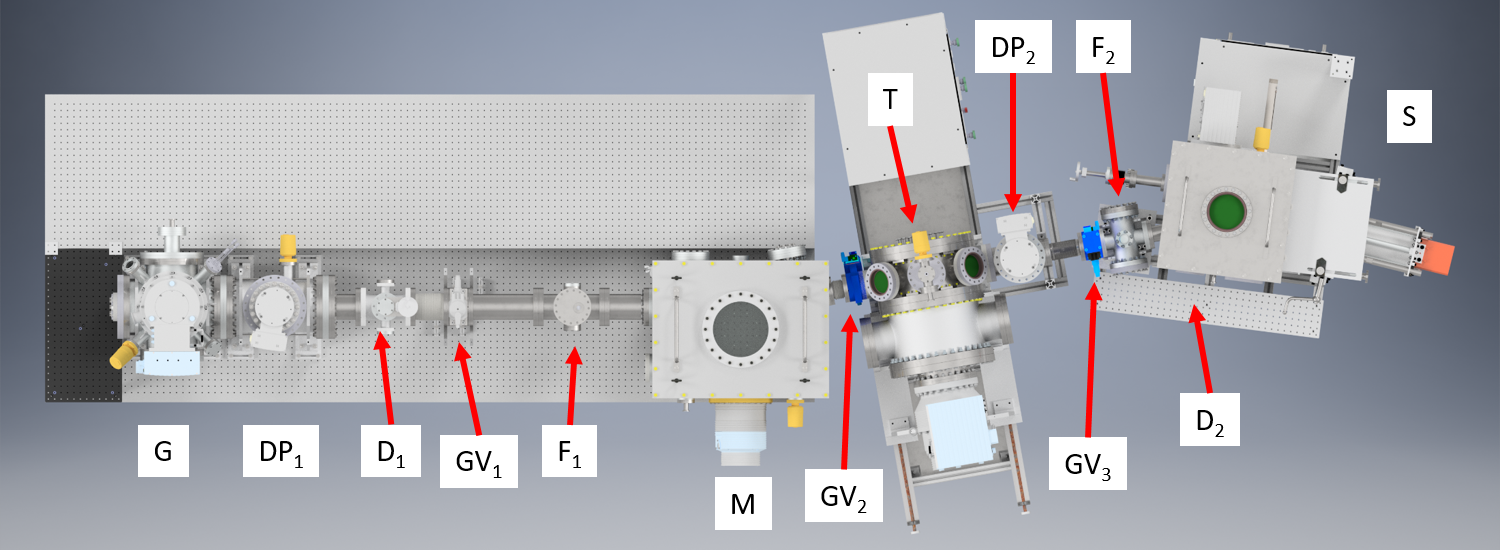
\includegraphics[width=1.0\textwidth]{figures/chap2/TABLe assembly - overhead labeled.png}
	\caption{Overhead rendering of the TABLe's vacuum chambers. In-air optics are omitted for visual clarity. G: generation chamber; DP: differential pumping chamber; D: IR diagnostic station; GV: gate valve, F: metal filter; M: mirror chamber; T: target chamber; S: XUV photon spectrometer.}
	\label{fig:TABLE_overhead_drawing}
	%  rendered using Inventor Studio (png). labels added in powerpoint
\end{sidewaysfigure}

\begin{sidewaysfigure}
	\centering
	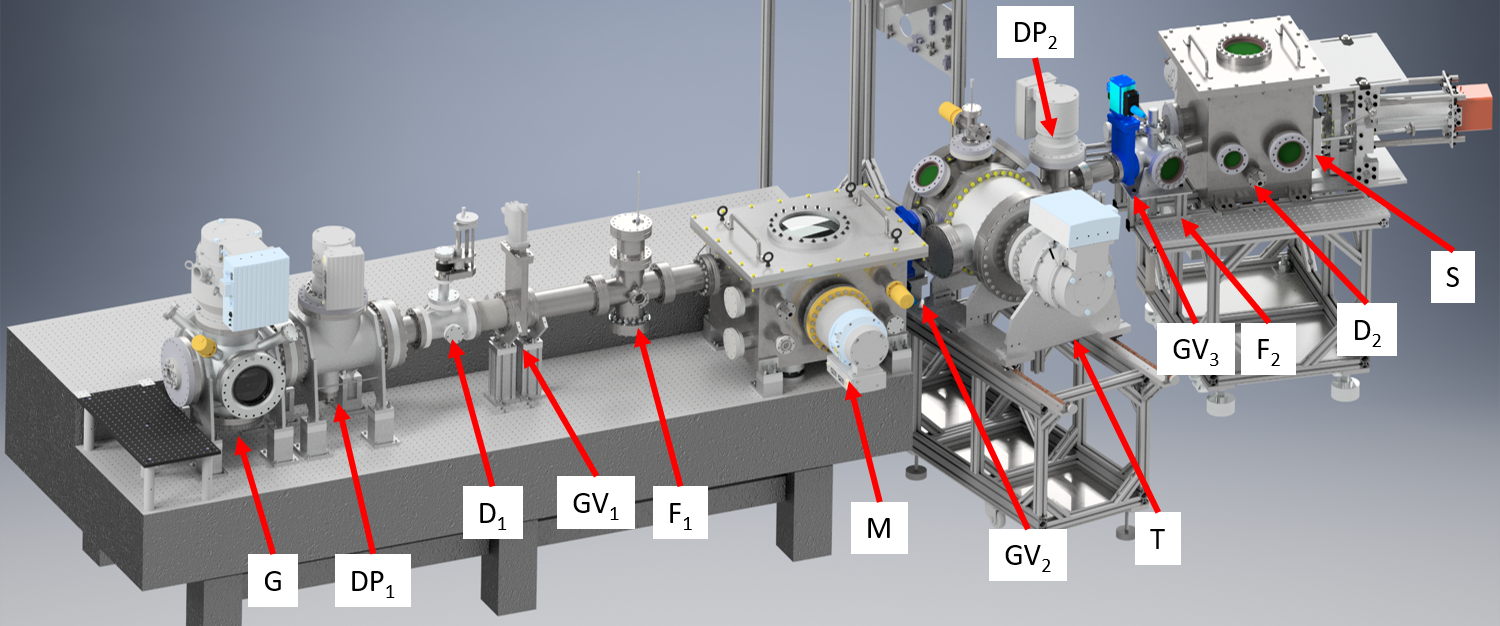
\includegraphics[width=1.0\textwidth]{figures/chap2/TABLe assembly - angled labeled.png}
	\caption{Angled rendering view of the TABLe's vacuum chambers showing the two-level 4' $\times$ 10' optical table. G: generation chamber; DP: differential pumping chamber; D: IR diagnostic station; GV: gate valve, F: metal filter; M: mirror chamber; T: target chamber; S: XUV photon spectrometer.}
	\label{fig:TABLE_angled_drawing}
	%  rendered using Inventor Studio (png). labels added in powerpoint
\end{sidewaysfigure}


In this section, we will provide a brief overview of each vacuum chamber in the TABLe vacuum system. Renders of the final vacuum design are shown in \cref{fig:TABLE_overhead_drawing,fig:TABLE_angled_drawing}. A cartoon of the beam path showing the beam path relative to the vacuum system is shown in \cref{fig:beamline_schematic}.

The first half of the vacuum system (generation, differential pumping, diagnostic station, \nth{1} metallic filter and mirror chambers) sits atop a custom split-level 4' $\times$ 10' optical table (TMC Vibration Control). The lower deck of the table is 24" wide and 12" thick and the upper deck is 20" thick. With this design, we are able to place the vacuum chambers directly on the lower deck while keeping the beam height of the in-air components at a standard height above the upper deck of the table. Like all other optical tables in the DiMauro lab, this table is not pneumatically floated; it sits directly on a steel leg assembly. This maintains the relative position between the optical tables and allows us to put the weight of the chambers on top of the table.

The second half of the vacuum system (target, differential pumping, \nth{2} metallic filter and spectrometer chambers) is not directly connected to the optical table, but instead sits on floor-mounted extruded aluminum frames. This modularity allows us to swap the endstations as dictated by experimental requirements. Although this makes these chambers less mechanically stable, this is an acceptable compromise as they are not part of the interferometer.

We use three gate valves to create four different vacuum regions in the beamline. This allows us to vent or pump down these sections independently, which is useful when trying to preserve air-sensitive components (MCP, metal filters, samples) or to minimize downtime when performing a ``quick fix" that neccessitates venting a single section. All three gate valves are electro-pneumatically powered so that they can be controlled via the OMRON safety system. GV$_1$ it is positioned between the IR diagnostic station and the metal filter, upstream of the ellipsoidal mirror. GV$_2$ is located between the mirror and target chambers. GV$_3$ is located between the target chamber's differential pump and the spectrometer's filter chamber. The four vacuum sections are colloquially referred to as the generation chamber, the mirror chamber, the target chamber and the spectrometer. Vacuum bellows are installed between the sections to facilitate chamber alignment.

Pressures in each chamber are monitored using a combination Pirahni / cold cathode pressure gauge (Leybold PTR90) that can read pressures from 750 Torr to $7.5 \times 10^{-9}$ Torr. Each vacuum section has a CF-to-KF adapter fitted with a blank KF flange, which is loosened while venting to prevent overpressurization of each vacuum section. The pressure in each turbo pump foreline is monitored by a thermocouple pressure gauge (Lesker KJL-6000) and analog controller.

\subsubsection{Generation and Differential Pump Chambers}

The first chamber in the vacuum system is the \textit{generation chamber} (G), where the XUV light is produced via HHG. Attached to this chamber and separated by a vacuum aperture is the \textit{differential pumping chamber} (DP$_1$). The geoemtry of these two chambers localizes the high gas pressures required for HHG within the generation chamber.

The generation chamber is designed to house the HHG gas nozzle or cell, and short focal length optics. It is here that the XUV light is created for the ATAS experiments. As such, it must be large enough to house an XYZ translation stage, as well as the neccessary electric and gas line feedthroughs. The turbo pump must be large enough to maintain milliTorr or lower pressures while being subjected to large gas throughputs for the duration of an experiment. The geometry of the chamber must accommodate a range of focal lengths and optical layouts. To facilitate IR/gas nozzle alignment, there must be a clear line of sight from outside the chamber to the IR's focal spot (roughly, the center of the generation chamber).

The generation chamber is a standard 6-way 10" ConFlat (CF) cross that has been modified by the Physics Machine Shop to have four additional 2.5" CF ports. These so-called radial ports are positioned at the corners of the top flange and are directed towards the center of the generation chamber. The 10" CF flanges are populated as follows. A large turbo pump (Oerlikon Leybold Turbovac Mag W 1300 iP, 1300 Liter/sec) is mounted on the top 10" CF flange. The bottom flange has a 50-pin electric feedthrough and tapped holes for mounting an internal aluminum breadboard, which holds the motorized XYZ manipulation stage, gas nozzle / cell, and any focusing optics. The front flange has zero length adapter with a custom o-ring sealed optical window mount (2" diameter, 1.5" clear aperture, 3 mm thick CaF\textsubscript{2}), which allows the laser light to be routed into the chamber. A large 8" diameter viewport is mounted on the right flange, and a CF-to-KF adapting flange for the HPC (see \cref{sec:HPC}) is mounted on the left flange. The rear flange holds the vacuum aperture assembly and a double-sided 10" CF flange, which connects to the front flange of the differential pump chamber. The 2.75" radial flanges hold a Leybold pressure gauge, a 2" diameter viewport and a 4-pipe 1/8" Swagelok gas feedthrough flange (Lesker).

The vacuum aperture assembly is modular, as it allows different sized apertures to be installed as neccessary. Currently, we use a 10 mm diameter aperture which was chosen to maximize the XUV transmission downstream. This setup yields a pressure drop of about 2 orders of magnitude across the aperture.

The differential pumping chamber is a standard 3-way 10" CF tee with two additional 2.75" CF flanges pointing towards the optical axis. The front 10" CF flange is connected to the generation chamber; the top CF 10" flange holds a small turbo pump (Oerlikon Leybold Turbovac Mag W 400 iP, 400 L/s) and the rear 10" CF flange connects to the IR diagnostic station. A KF blow-off assembly and a pressure gauge are mounted to the 2.75" CF flanges.

Typical operating pressures using a 200 $\mu$m diameter free expansion nozzle (Argon gas, $P_0 = -5$ psig backing pressure, 2.75 Torr-liter/second throughput) are about 3 mTorr in the generation chamber and $5 \times 10^{-5}$ Torr in the differential pump chamber.

\subsubsection{IR Diagnostic Station}

An \textit{IR diagnostic station} (D$_1$) is located after the differential pumping chamber. The diagnostic station houses a silver mirror mounted to a linear shift mechanism. When retracted, the mirror is out of the optical axis; when inserted the IR beam is diverted outside of the vacuum system through a window onto the upper deck of the split level optical table. This diagnostic station is used to measure the transmitted power of the generation arm when aligning the high pressure cell (HPC, see \cref{sec:HPC}).

\subsubsection{Filter Chamber}
\label{sec:filter_chamber}

\begin{figure}
	\centering
	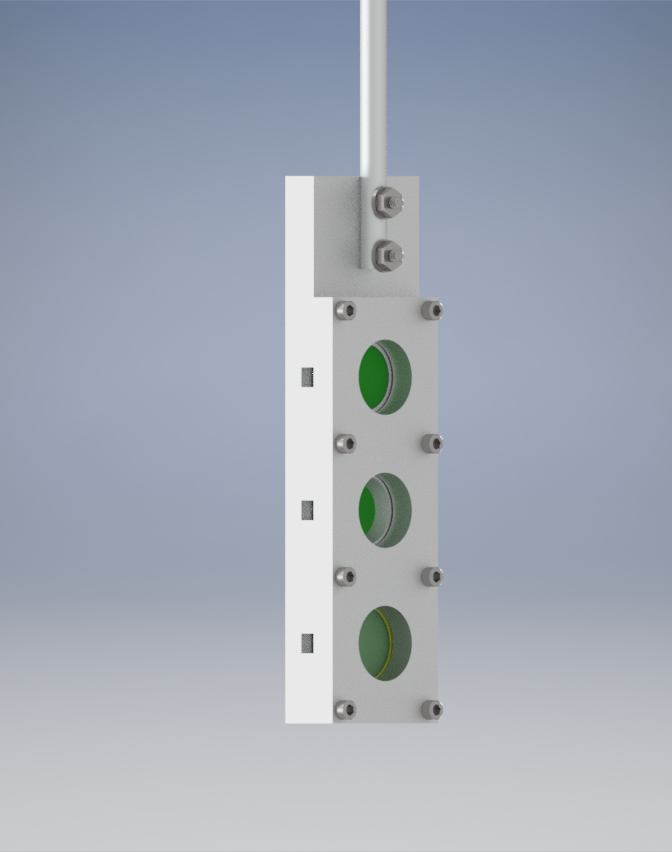
\includegraphics[width=0.50\textwidth]{figures/chap2/filter_stick.png}
	\caption{Rendering of the metallic filter assembly in the spectral filter chamber. Metallic filters are shown with a false green color for visual clarity.}
	\label{fig:filter_stick}
	% generated using Inventor Studio
\end{figure}

The generation arm's IR light is blocked at the first spectral \textit{filter chamber} F$_1$, which is located after the diagnostic station and before the XUV mirror. This chamber houses a o-ring sealed insertable rod upon which a clamshell assembly is mounted, as shown in \cref{fig:filter_stick}. This assembly was designed to hold standard metallic filters made by Luxel or Lebow, or achromatic MCP filters \cite{zhangSuppressionDrivingLaser2014}. By changing the insertion of the rod into the chamber, the user can select which of the three filters is on the optical axis. A calibrated indicator located outside the chamber (not shown) has markings to indicate the approximate rod position for each filter. The precise height of the filter can be fine tuned while observing the spatial profile of the XUV beam, as reported by the XUV spectrometer. Note that using a mesh-supported filter will imprint a grid-like pattern into the XUV beam, which will be apparent in the spectrometer's readings. Retracting the rod fully allows the XUV-IR beam to continue down the beamline unattenuated. Users should are cautioned that unattenuated IR light from the generation arm will destroy condensed matter samples in the target chamber.

\subsubsection{Mirror Chamber}

The \textit{mirror chamber} (M) is located after the filter chamber at the end of the 4' $\times$ 10' optical table. This chamber houses the ellipsoidal and hole mirrors (discussed in \cref{sec:Interferometer_Design}). The ellipsoidal mirror (EM) reimages the XUV source onto the target, while the hole mirror (HM) collinearly combines the generation arm's XUV with the pump arm's IR, closing the interferometer. The two pulses leave the chamber through the exit flange, which is angled 10 degrees to the left to account for the 85 degree incident angle of the EM.

This chamber has windowed ports (2 inch diameter, 3 mm thickness CaF\textsubscript{2}) that allow for positioning of the hole mirror before or after the ellipsoidal mirror, depending on experimental requirements. If the EM precedes the HM, then the IR pump arm focal parameters can be tuned arbitrarily, but this flexibility comes at the cost of having an additional optic in the interferometer. If the HM precedes the EM, then both the XUV and the IR pump share a common focusing optic which is outside the interferometer, which can improve interferometric stability.

\begin{figure}
	\centering
	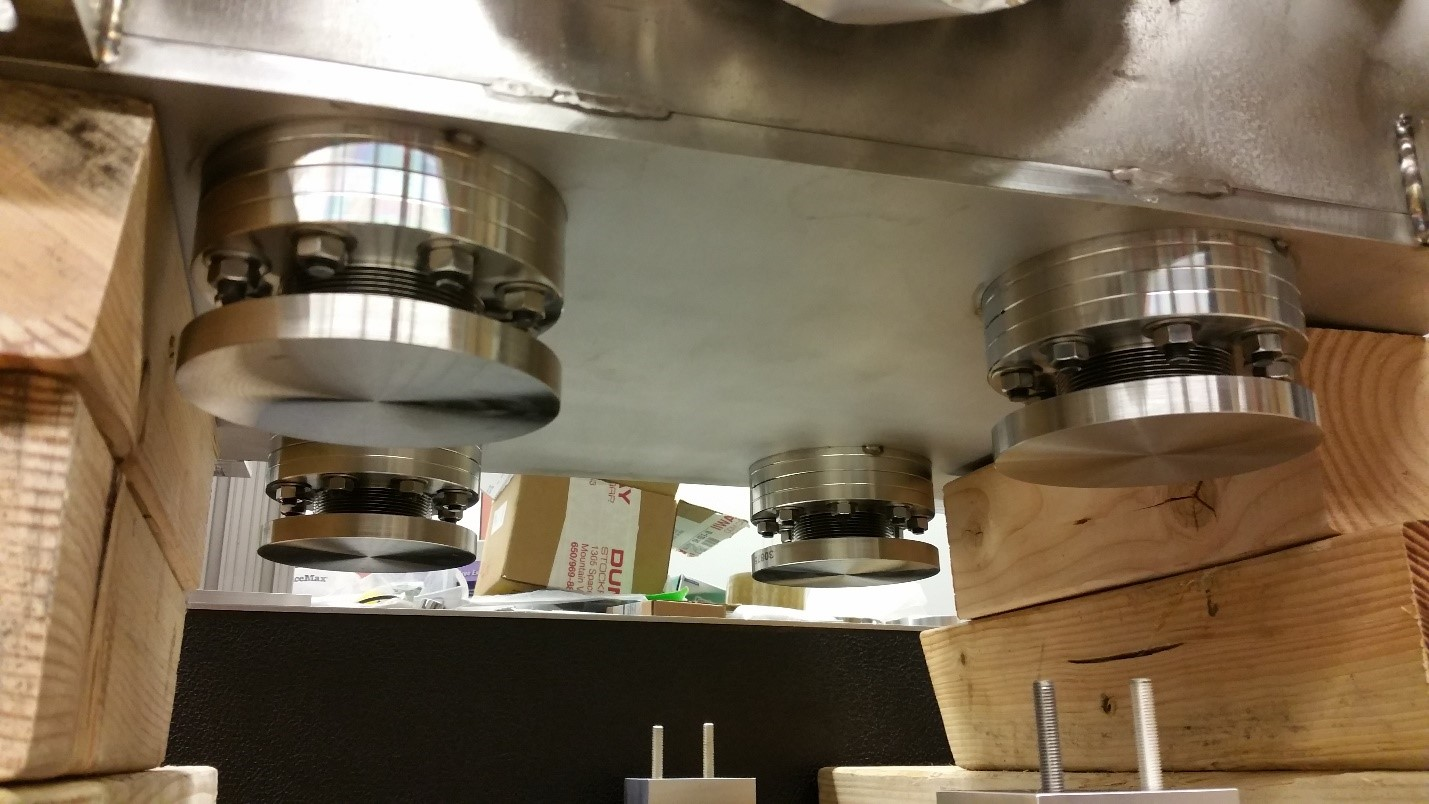
\includegraphics[width=0.75\textwidth]{figures/chap2/mirror_chamber-bellows_feet_lowres.jpg}
	\caption{Photograph of the underside of the mirror chamber during installation showing the vibration-dampening bellows. Steel rods (not visible) connect the interior of the bellows feet to the interior breadboard. After installation, the flat metal disks were secured to the optical table using clamps.}
	\label{fig:mirror_chamber_bellows_feet}
	% generated using Avant.CAD screenshot tool
\end{figure}

An internal reinforced aluminum breadboard supports the optomechanical components within the chamber. This breadboard is mechanically coupled directly to the 4' $\times$ 10' optical table using four stainless steel columns that run through openings on the underside of the mirror chamber, as shown in \cref{fig:mirror_chamber_bellows_feet}. Each port has a soft bellows housing that isolates chamber vibrations (originating from the pumping system) from the interferometrically stable optics within the chamber. 

\begin{figure}
	\centering
	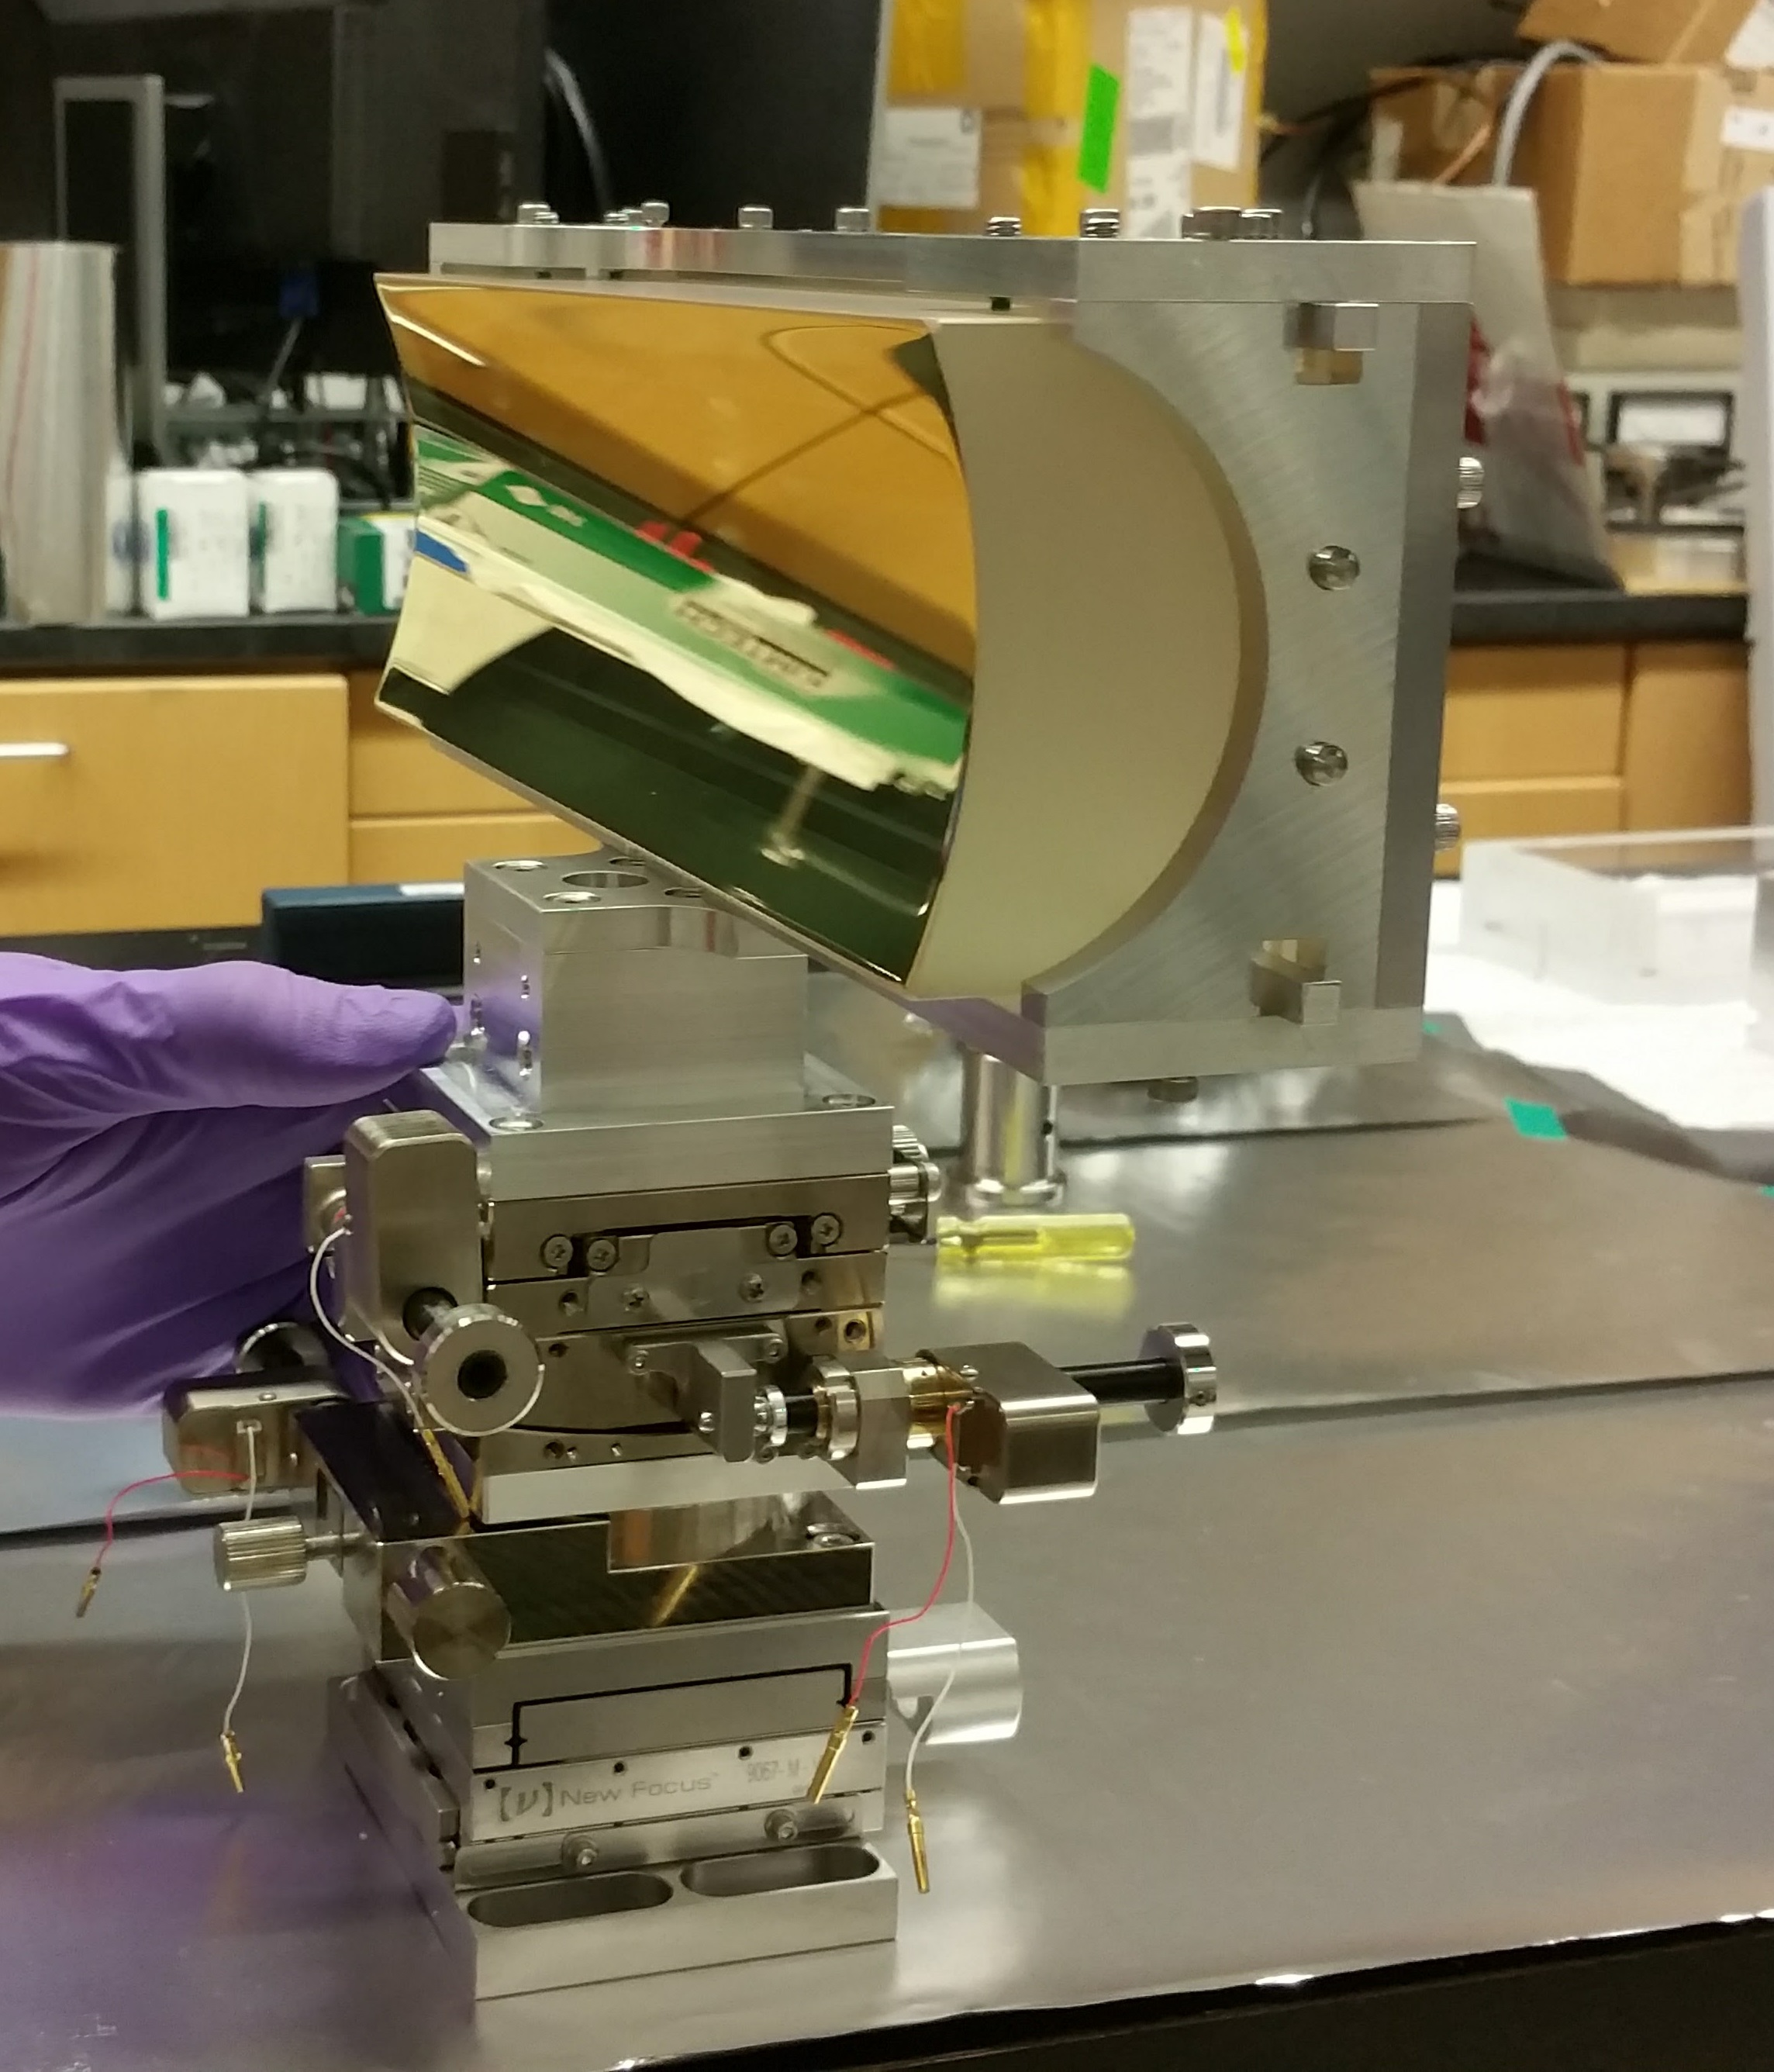
\includegraphics[width=0.75\textwidth]{figures/chap2/EM_in_mount.jpg}
	\caption{Photograph of the ellipsoidal mirror in its motorization stack prior to being installed in the mirror chamber.}
	\label{fig:EM_in_mount}
	% cropped version of 20160823_145837.jpg
\end{figure}

It is important to have remote \textit{in vacuo} control of both the EM and the HM, as the final alignment must be done with the XUV light. The optomechanical support of the ellipsoidal mirror was designed to avoid the cantilevering present in the XUV mirror of the RABBITT apparatus, which eliminates a source of mechanical instability. This required the use of custom vacuum compatible stages and spacers. To this end, the ellipsoidal mirror is placed atop a 5-axis vacuum compatible motorized stack, as shown in \cref{fig:EM_in_mount}. Starting from the breadboard, we have an XY crossed-roller bearing stage assembly (Newport) actuated by encoded stepper motors (Thorlabs). Next, a rotation stage (OptoSigma KSPS-606M-EN-N-2) controls the yaw. A matched pair of custom goniometers (OptoSigma, 85 \& 105 mm radii) with a center of rotation corresponding to the optical center of the ellipsoidal mirror, control the roll and pitch of the EM. All three rotations are actuated by picomotors (Newport 8301-UHV). An aluminum bracket, constructed of 7075 aluminum and manufactured by the Physics Machine Shop, surrounds the optically inactive sides of the ellipsoidal mirror and secures it to the top of the optomechanical stack. The height of the ellipsoidal mirror is fixed by the combined height of the breadboard, optomechanical stack and aluminum bracket.

The hole mirror is mounted in a 2 inch diameter gimballed beamsplitter holder (OptoSigma BHAN-50M-8-32UNC), modified to work with a pair of picomotors (Newport 8301-UHV) and to be vacuum compatible. This mount was chosen as it has a large clear aperture in both transmission and reflection at 45 degrees. This capability allows for the future implementation of an active interferometric control arm using a visible wavelength. The mirror chamber has two extra 4.5" CF ports for a future implementation of this control system.

\begin{figure}
	\centering
	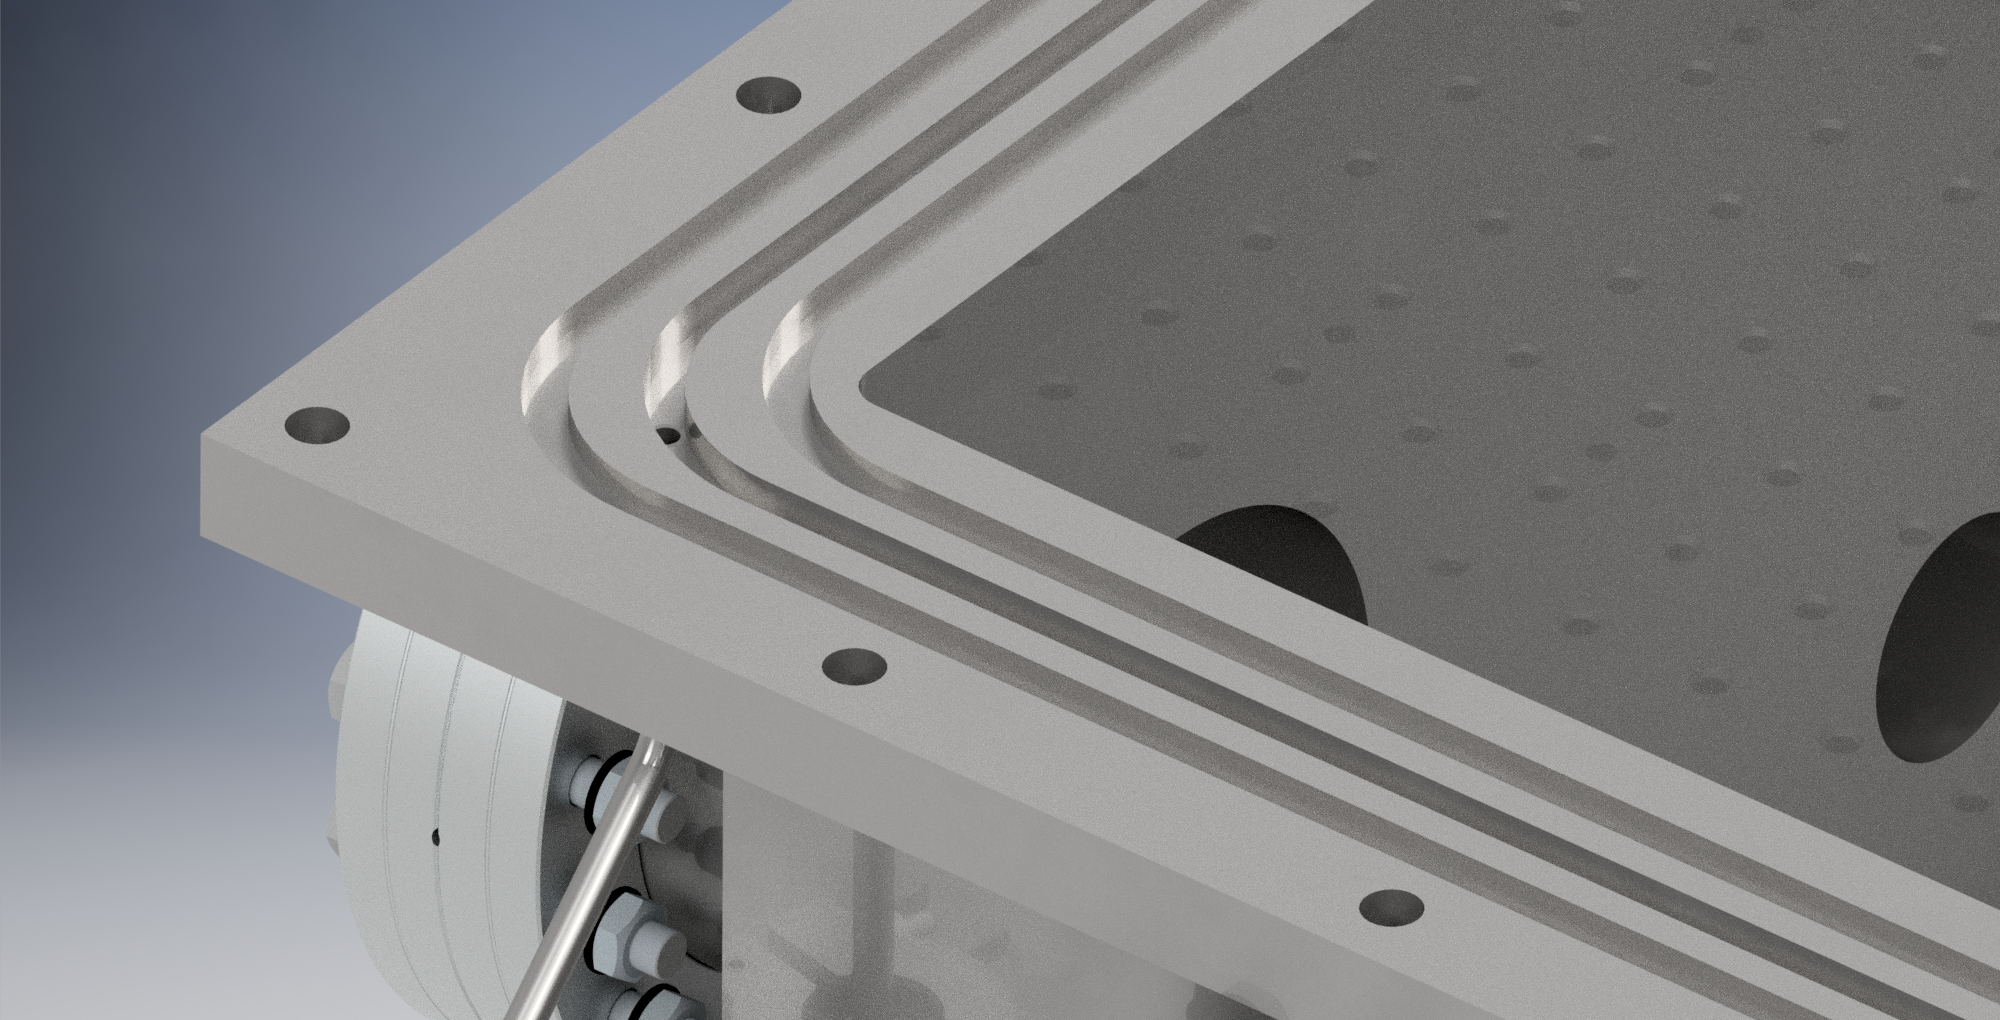
\includegraphics[width=0.75\textwidth]{figures/chap2/mirror_chamber-diff_pump_groove.png}
	\caption{Rendering of the mirror chamber's sealing surface showing detail of the differentially pumped double o-ring. O-rings are not shown in this figure. The two o-ring glands, the central pumping channel and the welded 1/4" stainless steel pumping tube are visible. Four through holes for the 5/16" sealing bolts are visible at the perimeter of the chamber's sealing surface.}
	\label{fig:mirror_chamber_diff_pump_groove}
	% generated using Avant.CAD screenshot tool
\end{figure}

The interior of the mirror chamber is accessed by removing the top panel, which was constructed from aluminum to reduce the weight. Nevertheless, the lid assembly weighs about 66 lbs (30 kg), so a manual winch was installed above the chamber so that any members of the group could remove the lid if neccessary. When installed, the lid is sealed to the chamber body by use of a differentially pumped double o-ring face seal, as shown in \cref{fig:mirror_chamber_diff_pump_groove}. Three grooves are milled into the stainless steel face of the chamber for this purpose; the outer and innermost channels each hold a large o-ring, while the middle channel is continously pumped via the beamline's rough vacuum system. The rough vacuum line splits before this turbo and provides pumping speed to both the turbo (Oerlikon Leybold Turbovac Mag W 700 iP) as well as the mirror chamber's differential groove.

\subsubsection{Target and \nth{2} Differential Pump Chambers}

The \textit{target chamber} (T) is located immediately after the mirror chamber, with the center of the chamber roughly corresponding to the XUV focal spot (750 mm from the ellipsoidal mirror). The chamber is an assembly of two 16" CF feedthrough collars populated with smaller radial flanges. The assembly is turned on its side so that the light enters and exits the chamber through the radial flanges.

The left collar has eight 6" CF radial flanges and serves as the interaction region. The interaction collar is mounted directly to the extruded aluminum frame (80/20 Inc.). The bottom radial flange supports an internal aluminum breadboard. The breadboard supports a motorized XYZ stage (Newport), upon which a sample holder can be attached. Encoded stepper motors (Thorlabs) are used for repeatable sample movement relative to the XUV/IR focus. The top radial port has a 6"-to-2.75" zero length reducer and a 2.75" CF tee which holds a KF blow off valve, a pressure gauge, and a gas line feedthrough for gas phase measurements. Viewports are installed on the two top diagonal radial ports. A 50-pin electrical feedthrough (Accuglass) is mounted on one of the bottom diagonal ports. The horizontal radial flanges serve as the entrance and exit ports for the light. A vacuum aperture (5 mm diameter) is mounted on the external side of the horizontal exit port to limit gas flow into the spectrometer chamber when gas phase experiments are performed. The left 16" CF flange holds a 16"-to-8" zero length adapter. Currently, this 8" port is used as an access port, but it was originally designed to accommodate an electron spectrometer to record simultaneous photon and electron measurements (not implemented).

The right collar has two 8" CF radial flanges which are used as access ports. A large turbo pump (Oerlikon Leybold Turbovac Mag W 1300 iP) is mounted via a 16"-to-10" reducing flange. The assembly was designed to be opened in the middle by breaking the 16" CF connection between the two collars. To facilitate this motion, the right collar and turbo pump are mounted to a rail system using sets of single and dual track roller bearings (Thomson).

The second differential pumping chamber (DP$_2$) is a 4.5"/6" reducing cross located immediately after the target chamber. A modified 6"-to-4.5" zero length reducing flange holds a 5 mm diameter vacuum aperture and connects the target and differential pumping chambers. This aperture size significantly reduces the IR flux and lowers the operating pressure in the photon spectrometer during gas phase measurements. An 8"-to-6" zero length reduces is used to connect a hybrid bearing turbo pump (Oerlikon Leybold Turbovac T450i) to the top of the DP$_2$ chamber.

An aluminum breadboard is mounted to the bottom radial flange at the center of the target chamber. A motorized crossed roller bearing XYZ stage (1" travel, Newport) sits atop the breadboard near the XUV-IR focal plane. A custom modular bracket is mounted to the stage and accepts a 3x3 condensed matter sample holder (3x3 grid of 5 mm circular clear apertures in a clamshell geometry) and / or a gas nozzle.

For additional details on the target and differential chambers, see Stephen Hageman's dissertation \cite{hagemanComplexAttosecondTransientAbsorption2020}.

\subsubsection{\nth{2} Filter and XUV Photon Spectrometer Chambers}

A second filter chamber (F$_2$), is located after the target differential pumping chamber. Designed to filter out the residual IR light from the pump arm, it is very similar to the first filter chamber (F$_1$). The main difference is that we use an UHV-rated linear actuactor (Lesker LBD35-150-H) to control the filter's position in the beam, rather than an o-ring seal, which allows the ultimate pressure of the spectrometer chamber to reach UHV. The target chamber's vacuum aperture and the spatial mode from the hole mirror largely make this filter unneccesary, as most of the energy is blocked before it reaches the filter chamber.

The photon spectrometer's optics and chamber were custom built to meet our experimental needs. Stephen Hageman's dissertation \cite{hagemanComplexAttosecondTransientAbsorption2020} and Sierra O'Bryan's thesis \cite{obryanHighResolutionXUV2015} contain detailed discussions on these subsystems. Below, we provide a brief overview of the vacuum chamber and the optomechanics. For a brief overview of the photon spectrometer's optical design, see \cref{sec:XUV_spectrometer}.

This chamber is a custom box design, with a removable lid sealed by a differential pumping groove similar to the mirror chamber. We have six-axis control over the positioning of the spectrometer's gratings. The gratings are mounted atop a 5-axis motion stack of linear, rotation and goniometric stages (Newport). The motion stack is mounted atop a linear insertion mount (Lesker LSM38-25-H), mounted on the floor of the chamber, which provides vertical translation via a manual, external control wheel.

A small turbo pump (Oerlikon Leybold Turbovac Mag W 400 iP) is mounted to the chamber wall in a horizontal configuration. An internal aluminum breadboard mounted to the floor and walls of the chamber provides support for ancillary optics, including diverting optics for external IR diagnostics. A linear actuator on the entrance wall pushes on a gearbox assembly to insert a 2" silver mirror into the beam path before the grating stack. When fully inserted, the beam is diverted out of the chamber through a viewport. An external breadboard, mounted to the chamber's extruded aluminum frame (8020 Inc.), holds IR diagnostic optics used for finding temporal overlap.

A third linear actuator mounted on the turbo pump wall inserts baffles between the grating and the XUV detector to block zero-order diffracted light. An 8" CF custom edge-welded bellows connects the exit chamber wall and the XUV detector flange assembly. A custom mechanical assembly (the ``cage and crank" system) provides three-axis control over the detector flange (horizontal translation, separation, and angle). This system allows us to optimize the grating-detector geometry, depending on which part of the XUV spectrum we want to resolve.

\textbf{Caution:} The bellows have a limited range of motion that is smaller than the cage and crank's range. It is possible to tear the bellows by moving the system outside its safe operation range. Even with the OMRON safety system armed, a tear in the bellows while under the system is under vacuum would lead to the sudden and catastrophic venting of the entire beamline. Refer to \cite{hagemanComplexAttosecondTransientAbsorption2020} and the bellows calculator for additional details before using this system.

\subsubsection{Rough Vacuum Details and OMRON Safety System}
\label{sec:rough_vacuum_details}

\begin{sidewaysfigure}
	\centering
	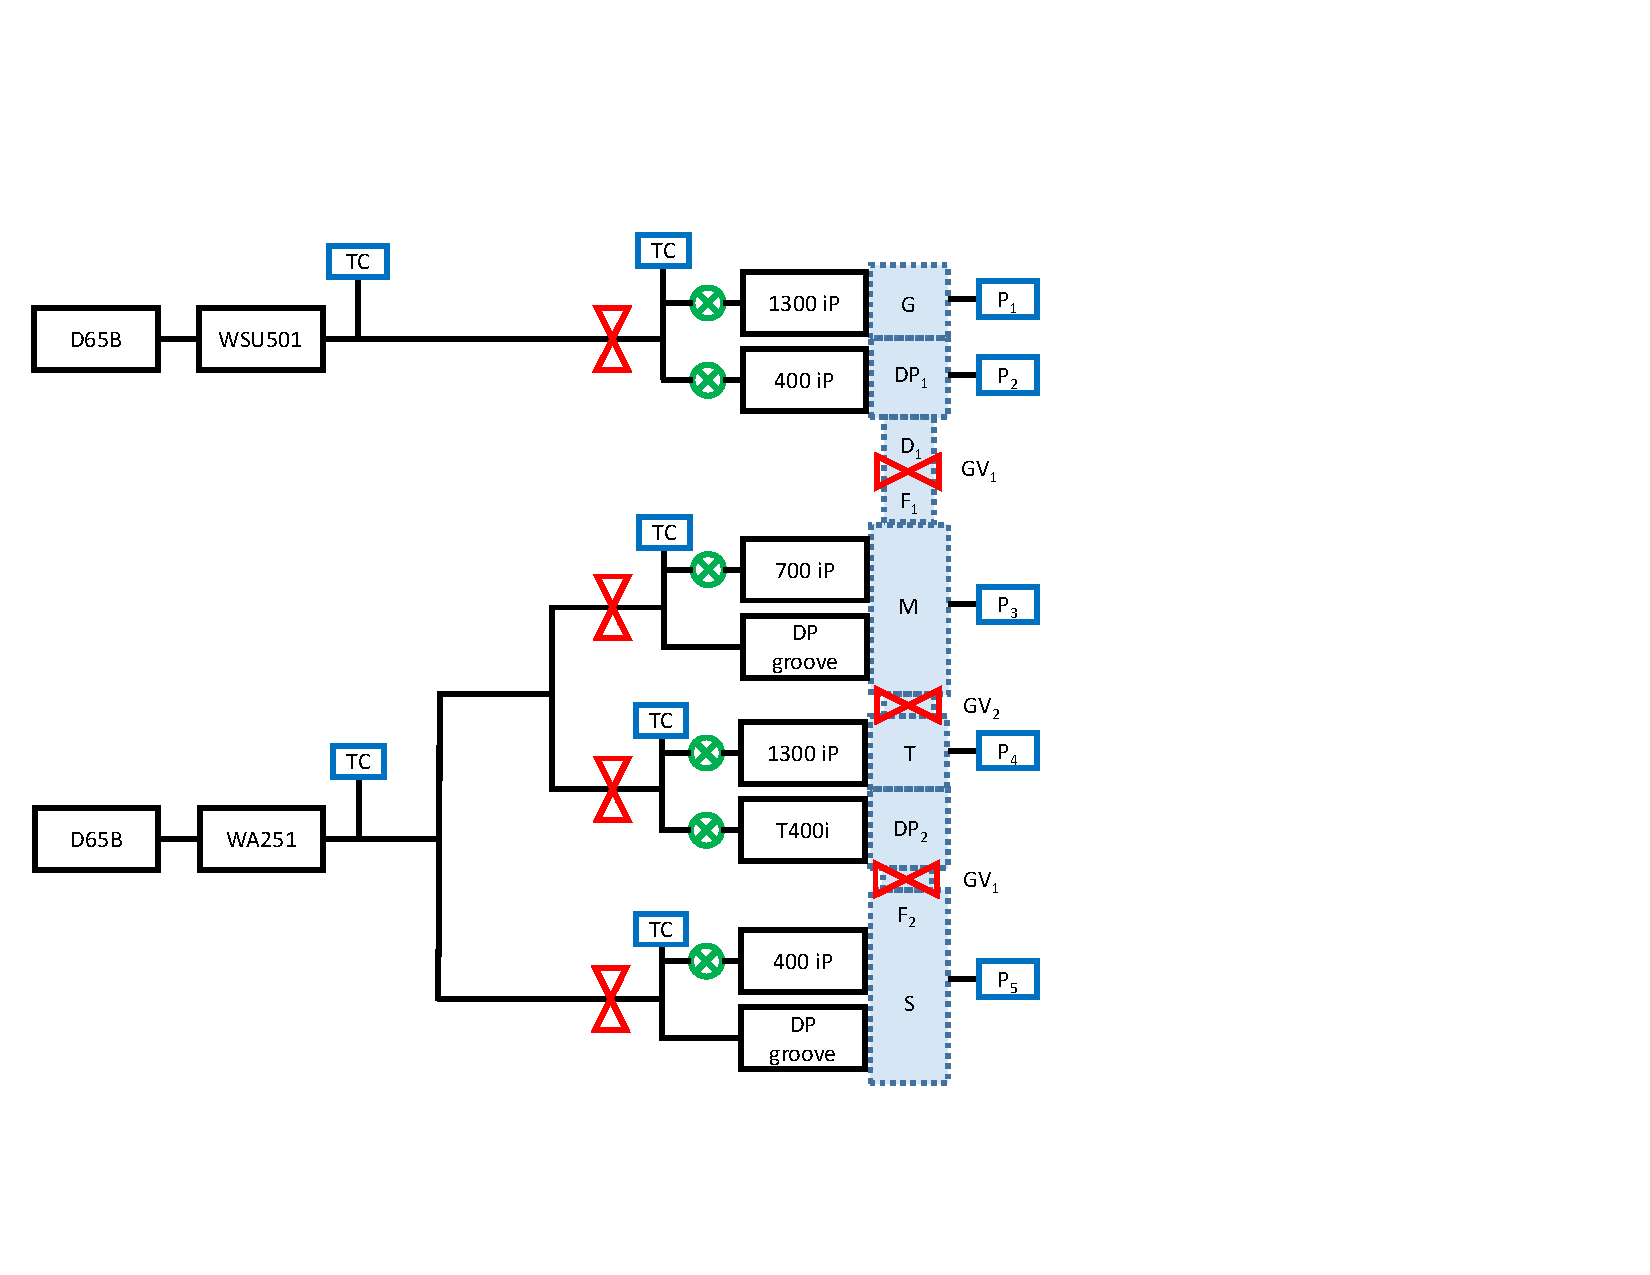
\includegraphics[width=0.75\textwidth]{figures/chap2/rough_vacuum_schematic.pdf}
	\caption{Block diagram of the TABLE's rough vacuum system showing rough and turbo pumps, control valves and pressure gauges. TC: thermocouple pressure gauge; P: UHV pressure gauge; $\otimes$: manual valve, $\bowtie$: rough vacuum solenoid or UHV pneumatic gate valve. UHV is indicated by blue shaded region. G: generation chamber, DP: differential pumping chamber, M: mirror chamber, T: target chamber, S: photon spectrometer chamber.}
	\label{fig:rough_vacuum_schematic}
\end{sidewaysfigure}

The turbo pumps are backed by a pair of rough vacuum systems that are located in an adjacent pump room. A schematic of the system is shown in \cref{fig:rough_vacuum_schematic}. The generation and differential pumping chambers share a high throughput system, and the remaining chambers (mirror, target, target differential pumping, spectrometer) share a smaller system.

The large rough pump system consists of a rotary vane (RV, Leybold D65B, 65 m$^3$/hr) and roots blower (Leybold WSU 501, 500 m$^3$/hr) pump stack. This rough vacuum system is connected to the beamline via a large diameter copper and PVC tube. The pressure at the inlet flange of the roots blower is remotely monitored using a thermocouple gauge (Agilent Type 0531 TC), an electronic gauge controller (Lesker KJL615TC-E), a wireless networking router, and a touchscreen-enabled Raspberry Pi running a web applet (Kurt J. Lesker).

The smaller system uses the same model RV pump, but a smaller roots blower (Leybold WA 251, 250 m$^3$/hr). Although it has half the pumping speed as the generation pump stack, the gas load for these chambers is minimal compared to the generation chamber. The pressure at the inlet flange of the roots blower is remotely monitored using a copy of the system that monitors the generation roots blower pressure.

Owing to the complexity of the vacuum system, we decided to implement a ``safety system", i.e., a programmable logic controller that controls the major components of the vacuum apparatus. The heart of this system is an OMRON PLC. Its design follows that of the RABBITT apparatus \cite{chirlaAttosecondPulseGeneration2011}, although the new system controls significantly more equipment that its predecessor. Special thanks go to Andrew Piper \cite{piperAndrewPiperDissertation2022}, who programmed and implemented this system on our beamline. A full user manual is available on the group drive, and a quick start guide is available in \cref{sec:OMRON_instructions}. In short, the OMRON safety system monitors the setpoints of the 5 UHV pressure gauges and controls the 6 turbo pumps, the 4 rough vacuum solenoid gate valves, the 3 UHV pneumatic gate valves and the 5 turbo pump solenoid vent valves according to a simple set of logic rules. This automation enables three main features. First, the user can pump down or vent individual sections (or the entire beamline) with a few button presses. With the exception of actuating the manual valves and the KF blow off flanges, this process is almost entirely automated which greatly reduces the complexity of using the vacuum system. Second, the OMRON verifies that there is no pressure differential across the UHV gate valves before they are opened. If the pressure on either side of the gate valve is above a setpoint, the OMRON will prevent it from opening. Finally, when the OMRON is armed, it will monitor the pressure in each chamber and perform an emergency shutdown/vent procedure if any pressure gauge reports pressures above a setpoint. In the event of a pump failure, the armed OMRON system will safely vent the beamline without any user intervention.

\section{XUV Optics}
\label{sec:Interferometer_Design}

\begin{figure}
	\centering
	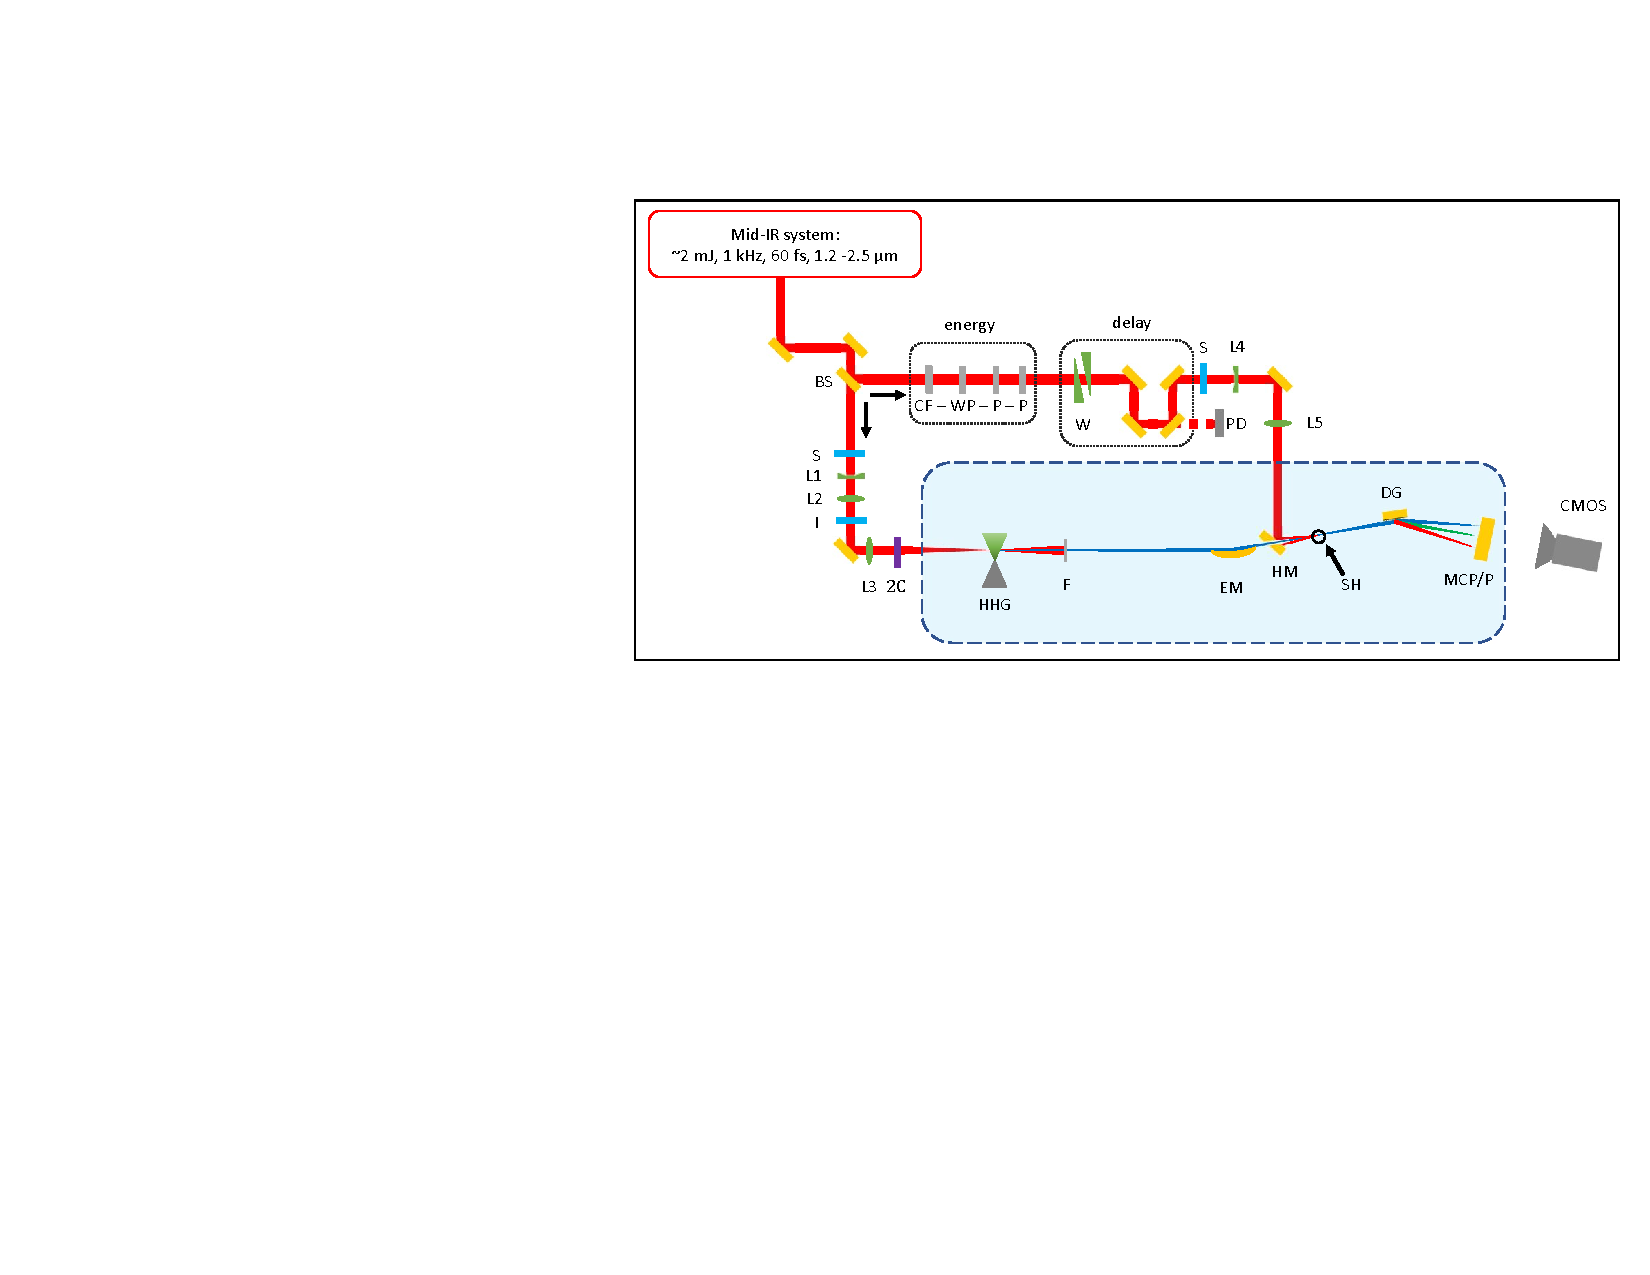
\includegraphics[width=0.95\textwidth]{figures/chap2/beamline_schematic.pdf}
	\caption{Schematic of the Transient Absorption BeamLine (TABLe). Blue shaded region represents vacuum. BS: beam splitter, S: computer-controlled shutter, L: lens, I: iris, 2C: optics for two-color generation, HHG: high harmonic generation, F: metallic filter, EM: ellipsoidal mirror, HM: hole mirror, SH: sample holder, CF: long-pass color filter, WP: $\lambda/2$ waveplate, P: wire-grid polarizer, W: delay wedges, PD: photodiode and associated optics, DG: dispersive grating, MCP/P: micro-channel plate and phosphor.}
	\label{fig:beamline_schematic}
\end{figure}

In this section, we will discuss the XUV optical design of the TABLe system. We start with a statement of the design goals, followed by a general discussion of XUV focusing optics to motivate our choice of the Zeiss gold coated ellipsoidal mirror. 

\subsection{Design Goals}

We started with several design requirements. First, we wanted to be able to deliver XUV light onto the sample with photon energies as high as 300 eV, which would enable us to study carbon containing materials such as graphene. However, we also wanted to preserve the lower energy portion of the harmonic spectrum, allowing the study of semiconductor and transition metal compounds. This broadband requirement restricts us to metal-coated reflective optics.

Condensed matter ATAS experiments have significantly higher XUV flux requirements compared to RABBITT experiments. This meant that our XUV focusing solution needed to have the highest reflectivity possible, and we needed to minimize any XUV losses elsewhere in the beamline. This restricts us to single optic solutions, and puts stringent requirements on the smoothness of the optic.

The IR intensity profile at the focus is an important parameter for every experiment. In a transient absorption experiment, the experimental signal originates from the spatial overlap of the sample, the XUV and the IR light in the interaction region. Ideally, neither pulse would have any spatial structure at the interaction plane. In the real world, we design the optics to minimize the intensity variation of the IR over the spatial extent of the XUV spot. For finite beam sizes, this is accomplished by focusing the XUV tighter than the IR while minimizing aberrations.

Although the primary scientific goal for this work was transient absorption experiments in condensed matter, the requirements of other experiments were considered during the design phase of the apparatus. Aside from general modularity, we wanted the beamline to be able to study strong field physics in helium, which has an IR intensity requirement in the target chamber on the order of $10^{14}$ W/cm\textsuperscript{2}. These intensities are neither required nor desired for condensed matter ATAS experiments, as sample damage can easily occur in condensed phase materials around  $10^{12}$ W/cm\textsuperscript{2}. We chose to demagnify the XUV spot size by a factor of three, which reduces the XUV spot area by a factor of nine. This allows us to more strongly focus the IR pump pulse, resulting in a nine-fold increase of interaction intensity without changing the relative spot sizes of the XUV and the IR. This allowed us to reach our goal of $10^{14}$ W/cm\textsuperscript{2} for the doubly ionized helium gas for $e-2e$ experiments \cite{kiesewetterDynamicsNearThresholdAttosecond2019}.

%We can achieve $10^{14}$ W/cm\textsuperscript{2} by tightly focusing the output of the Spitfire laser system. However, we must reserve a significant amount of pulse energy for the HHG process. Secondly, the XUV spot size needs to remain smaller than the IR spot size to minimize IR intensity variation across the XUV-induced ionization volume. Thus, higher IR intensities can be achieved only if our XUV optic demagnifies the harmonic light source.

As we will discuss below, we are restricted to a reflective focusing geometry. As such, one relevant parameter is the ratio of the entrance and exit arms of the XUV optic. A desire to have modular endstations put a lower limit on the XUV optic's exit arm; too short and the mirror chamber would have to merge with the target chamber. Likewise, the footprint of the beamline had to fit within the south east target room, which put constraints on the length of the entrance arm.



\subsubsection{Reflective Optics}

The XUV light is divergent after its generation and needs to be focused onto a sample for the experiment. The short relatively wavelength of the XUV puts strong requirements on the surface quality of the focusing optic, raising the cost and manufacturing time significantly. Alignment of the optic is frustrated by the need for in-vacuum propagation and the invisible nature of XUV light. These factors lead us to pursue a ``one size fits all" broadband optic rather than a series of interchangeable narrow bandwidth optics tailored for individual experiments.

The presence of strong absorption edges over the bandwidth of the XUV pulse precludes the use of transmissive optics for most applications. Narrow bandwidth transmissive optics have been designed to exploit the dispersion near an absorption edge \cite{drescherExtremeultravioletRefractiveOptics2018}. However, these techniques cannot be extended to support the entire bandwidth of our XUV pulses. Reflective dielectric coatings have been designed for the XUV but they have a bandwidth of only $10-20$ eV \cite{kiesewetterDynamicsNearThresholdAttosecond2019}. These considerations leave reflective optics as the only good choice for broadband XUV light.

%The IR intensity profile at the focus is an important parameter for every experiment. In a transient absorption experiment, the experimental signal originates from the spatial overlap of the sample, the XUV and the IR light in the interaction region. Ideally, neither pulse would have any spatial structure at the interaction plane. In the real world, we design the optics to minimize the intensity variation of the IR over the spatial extent of the XUV spot. For finite beam sizes, this is accomplished by focusing the XUV tighter than the IR while minimizing aberrations. We chose to demagnify the XUV spot size by a factor of three, which reduces the XUV spot area by a factor of nine. This allows us to more strongly focus the IR pump pulse, resulting in a nine-fold increase of interaction intensity without changing the relative spot sizes of the XUV and the IR. While not required for a condensed matter experiment, the increased IR intensity was essential to doubly ionize helium gas for $e-2e$ experiments \cite{kiesewetterDynamicsNearThresholdAttosecond2019}.

XUV and x-ray reflective optics consist of highly polished curved substrates with a thin (typically 40 nm) metal coating applied to the polished surface. As a reflective optic, the precise shape of the surface (discussed below) determines the focusing properties, and the coating influences the spectral reflectivity and overall performance. The high tolerances and custom nature of these optics makes them very expensive (tens of thousands of dollars) with a long manufacturing lead time (12 months), so it was important to make an informed decision about this purchase. In the following sections we will briefly introduce the physics relevant to XUV optics, namely Fresnel reflection from a rough surface. We will use these results to motivate the selection of our XUV optic.

\subsection{Fresnel Reflection from a Rough Surface}

We use the familiar Fresnel equations to model reflection from the surface of a conductive surface \cite{zangwillModernElectrodynamics2013}. In the equations that follow, the vacuum is denoted by $j=1$ and the conductive material is $j=2$. The incident electric field is $E_I$ and the reflected component is $E_R$. We use the standard convention to denote the polarization\footnote{The designations $s$ and $p$ follow from the German words for perpendicular (\textit{senkrecht}) and parallel (\textit{parallele}).}: $p$-polarized light has an incident electric field parallel to the plane of incidence; $s$-polarized has an incident electric field perpendicular to the plane \cite{attwoodSoftXraysExtreme2000}. The complex reflection amplitudes $\hat{r}_{s,p}$ are written in terms of the complex impedance $\hat{Z}_j = \mu_j c / \hat{n}_j$ and the angle measured from the normal in each medium $\theta_j$:
\begin{equation}
\hat{r}_s \equiv \left[ \frac{E_R}{E_I} \right]_s = \frac{\hat{Z}_2 \cos \theta_1 - \hat{Z}_1 \cos \theta_2}{\hat{Z}_2 \cos \theta_1 + \hat{Z}_1 \cos \theta_2}
\label{eqn:Fresnel_rs_1}
\end{equation}
\begin{equation}
\hat{r}_p \equiv \left[ \frac{E_R}{E_I} \right]_p = \frac{\hat{Z}_1 \cos \theta_1 - \hat{Z}_2 \cos \theta_2}{\hat{Z}_1 \cos \theta_1 + \hat{Z}_2 \cos \theta_2}
\label{eqn:Fresnel_rp_1}
\end{equation}
Next, we assume non-magnetic media ($\mu_1=\mu_2=\mu_0$) and that the initial medium is vacuum ($\hat{n}_1 = 1$). We can express the reflection amplitudes using the complex index of refraction $\hat{n}_2 = n_2 + i k_2$:
\begin{equation}
\hat{r}_s = \frac{ \cos \theta_1 - \hat{n}_2 \cos \theta_2}{ \cos \theta_1 - \hat{n}_2 \cos \theta_2}
\label{eqn:Fresnel_rs_2}
\end{equation}
\begin{equation}
\hat{r}_p = \frac{ \cos \theta_2 - \hat{n}_2 \cos \theta_1}{ \cos \theta_2 + \hat{n}_2 \cos \theta_1}
\label{eqn:Fresnel_rp_2}
\end{equation}
The reflectance $R$ is the modulus squared of the reflection amplitudes:
\begin{equation}
R_s = \left| \frac{ \cos \theta_i - \hat{n}_2 \cos \theta_t}{ \cos \theta_i - \hat{n}_2 \cos \theta_t} \right|^2
\label{eqn:Fresnel_Rs_1}
\end{equation}
\begin{equation}
R_p = \left| \frac{ \cos \theta_t - \hat{n}_2 \cos \theta_i}{ \cos \theta_t + \hat{n}_2 \cos \theta_i} \right|^2
\label{eqn:Fresnel_Rp_1}
\end{equation}
%Finally, we assume that the first medium is vacuum ($\hat{n}_1 = 1$) and apply Snell's law to write the transmitted angle $\theta_2$ in terms of the incident angle $\theta_1$:
%
%\begin{equation}
%\hat{R}_s = \left| \frac{\cos \theta_1 - \hat{n}_2 \sqrt{1-\left(\frac{1}{n_2}\sin \theta_1\right)^2}}{\cos \theta_1 + \hat{n}_2 \sqrt{1-\left(\frac{1}{n_2}\sin \theta_1\right)^2}} \right|^2
%\label{eqn:Fresnel_Rs_2}
%\end{equation}
%
%\begin{equation}
%\hat{R}_p = \left| \frac{\sqrt{1-\left(\frac{1}{n_2}\sin \theta_1\right)^2} - \hat{n}_2 \cos \theta_1}{\sqrt{1-\left(\frac{1}{n_2}\sin \theta_1\right)^2} + \hat{n}_2 \cos \theta_1} \right|^2
%\label{eqn:Fresnel_Rp_2}
%\end{equation}

We introduce the \textit{glancing angle} $\phi \equiv \pi/2 - \theta$, which is the compliment to $\theta$. Total external reflection, where the incident rays do not penetrate the medium but rather propagate along the interface at angle $\phi_2 = 0$, occurs at incident glancing angles below the \textit{critical incident angle} $\phi_c$:
\begin{equation}
\cos \phi_c = 1 - \delta
\end{equation}
where $\delta$ is defined via  $\tilde{n} = (1-\delta) - i \beta$. The x-ray optics literature often makes approximations to the above reflectance equations using either the small angle approximation ($\delta \ll 1$ and $\cos \phi_c \sim 1$, or $\phi_1 \ll 1$), or the assumption that we are operating near the critical angle ($\phi_1 \sim \phi_c$) \cite{attwoodSoftXraysExtreme2000}. Note these assumptions are not neccessarily true for our geometry, especially at photon energies below 200 eV, where the critical angle for gold exceeds 10 degrees.

The above is valid for a perfectly smooth interface, but real optics have finite roughness. The effect of surface roughness on the reflection amplitude $\hat{r}$ is commonly treated by either the \textit{Debye-Waller} or \textit{N\'evot-Croce} factors. The relative sizes of the extinction length ($1/k_2$) and the in-plane characteristic length scale ($\delta r$) of the surface roughness determine which formalism is appropriate \cite{sentenacStatisticalAspectsWave2009, gibaudSpecularReflectivitySmooth2009}. For XUV light at a grazing angle on a gold surface, the extinction length is on the order of 10 nm, which is much smaller than the length scale of the surface roughness of highly polished materials (micron or mm scale). In this case, $\delta r$ is large enough for the incident and reflected fields have a precise phase relationship and the Debye-Waller formalism is appropriate \cite{stoevReviewGrazingIncidence1999}. Thus, the reflectance of our mirror can be modelled as:
\begin{equation}
\hat{r}^{\textrm{rough}} = \hat{r}^{\textrm{smooth}} \exp \left( -2 k_{1,z}^2 \langle z^2 \rangle \right)
\label{eqn:DW_2}
\end{equation}
where $ \langle z^2 \rangle$ is the variance of the interface height and $k_{1,z} = 2 \pi \cos \theta_i / \lambda$ is the normal component of the wave vector in medium 1 (in our case, vacuum). To get a sense of scale, a high quality off-the-shelf optic will have a surface roughness of $\langle z^2 \rangle = \lambda/10 = 63.2 \text{ nm}$, which is 5 times larger than the wavelength of a 100 eV photon. It is clear that we need to take advantage of specialized manufacturing techqniques while working in the XUV. Below, we apply this basic framework to guide the selection of the basic materials and geometric properties of our XUV focusing optic. 

\subsubsection{The Metallic Coating}

%Combining \cref{eqn:Fresnel_Rs_2,eqn:Fresnel_Rp_2} with \cref{eqn:DW_2} yields the reflectance of a rough metallic surface:
%
%\begin{equation}
%\hat{R}_s = \left| \frac{\cos \theta_1 - \hat{n}_2 \sqrt{1-\left(\frac{1}{n_2}\sin \theta_1\right)^2}}{\cos \theta_1 + \hat{n}_2 \sqrt{1-\left(\frac{1}{n_2}\sin \theta_1\right)^2}} \right|^2 \left( \frac{2 \pi \sigma \cos \theta_1}{\lambda} \right)^2
%\label{eqn:Fresnel_Rs_3}
%\end{equation}
%
%\begin{equation}
%\hat{R}_p = \left| \frac{\sqrt{1-\left(\frac{1}{n_2}\sin \theta_1\right)^2} - \hat{n}_2 \cos \theta_1}{\sqrt{1-\left(\frac{1}{n_2}\sin \theta_1\right)^2} + \hat{n}_2 \cos \theta_1} \right|^2 \left( \frac{2 \pi \sigma \cos \theta_1}{\lambda} \right)^2
%\label{eqn:Fresnel_Rp_3}
%\end{equation}
%The mid spatial frequency roughness (MSFR) of the ellipsoidal mirror's surface is $\le0.3$ nm when sampled at a spatial frequency of 1-200 $\mu m$.
%- the extinction length for photon range 30 - 500 eV in gold is on the order of 0.07 - 0.2 nm.
%- the 0.3 nm rms roughness is based on a measurement frequency of 1 - 200 microns. this corresponds to a relatively long-range / slowly varying roughness.
%- therefore we should use the debye-waller factor.
%
%Nevot-Croce model assumes random vertical roughness with a Gaussian distribution. for the low spatial frequencies of the roughness spectrum, the Fresnel reflection coefficient is usually multiplied with a Debye-Waller factor $\exp\left(-16 \pi^2 k_1^2 \sigma^2\right)$, while for the high spatial frequencies, the correction coefficient is given by the Nevot-Croce correction factor $\exp\left(-16 \pi^2 k_1 k_2 \sigma^2\right)$, where $\sigma$ is the root-mean-square (rms) of the vertical roughness, and $k_1$ and $k_2$ are the normal components of the wave-vectors in the two media \cite{stoevReviewGrazingIncidence1999}.

\begin{figure}
	\centering
	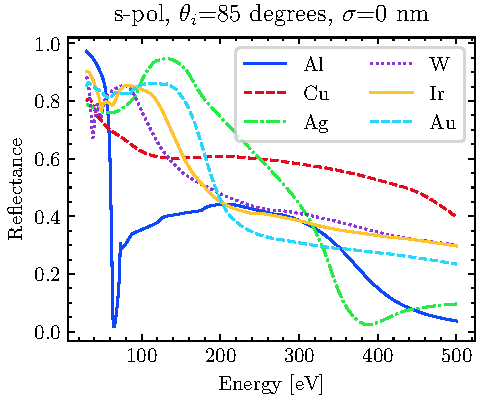
\includegraphics[width=0.75\textwidth]{figures/chap2/Fresnel_NoSigma.pdf}
	\caption{Fresnel reflectance for s-polarized light on smooth metal mirrors at a grazing angle of 5 degrees. Refractive index data obtained from \cite{gulliksonCXROXRayInteractions,henkeXRayInteractionsPhotoabsorption1993}. Calculation follows \cref{eqn:Fresnel_Rs_1,eqn:DW_2}.}
	\label{fig:Mirror_Material_Choice}
	% generated using \Python Scripts\CXRO\Fresnel.py
\end{figure}


\cref{fig:Mirror_Material_Choice} shows the Fresnel reflectance for various materials at a fixed 5 degree grazing angle (85 degree incident angle). From this figure, we can see that the materials properties strongly influence mirror perforance at these energies. Aluminum (Al) has a sharp absorption feature at 72 eV which is undesirable for a reflective optic; tungsten (W) and iridium (Ir) have extended spectral features between 35 and 50 eV. Silver (Ag) has the best reflectance below 250 eV. Copper (Cu) has the flattest performance out to 400 eV, with very few spectral features. Gold (Au) has good performance below 200 eV and a relatively flat spectral response outside the 150 - 200 eV region. 

Gold, silver and copper are good candidates for our desired spectral range. However, silver and copper can tarnish when exposed to atmosphere, which would change their reflectivity over time. Although the optic will be stored under vacuum, it will inevitably be exposed to air during transport, installation and whenever the beamline is vented. Due to the extremely thin and fragile optical coating, it is not possible to clean the XUV optic if it becomes dirty, damaged or tarnished. Gold was chosen to maximize the lifetime of the optic.

\begin{figure}
	\centering
	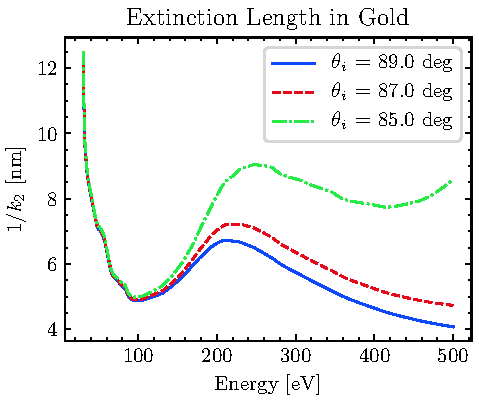
\includegraphics[width=0.75\textwidth]{figures/chap2/Au_ExtinctionLength.pdf}
	\caption{Extinction length in gold at various incident angles. Refractive index data obtained from \cite{gulliksonCXROXRayInteractions,henkeXRayInteractionsPhotoabsorption1993}.}
	\label{fig:Au_Extinction_Length}
	% generated using Fresnel.py
\end{figure}

The Fresnel analysis used above is valid for an infinitely thick medium, but one must question whether this is valid for a thin film gold coating. To answer this question, we plot the extinction length ($1/k_2$) in \cref{fig:Au_Extinction_Length}, with $k_2$ defined as ${ k_2 = \left( 2 \pi / \lambda \right) \sqrt{ \sin \theta_i^2 - \Re\hat{n}_2} }$ \cite{zangwillModernElectrodynamics2013}. We can see that above 30 eV, the extinction length remains below 13 nm; above 40 eV the extinction length is bounded by 10 nm. Based on this information, we decided to use the standard 40 nm coating offered by Zeiss. An adhesion layer (Cr) was applied to the substrate to prevent flaking of the gold coating. It should be noted that over time, the adhesion layer will diffuse into the gold and change the reflectivity.

\begin{figure}
	\centering
	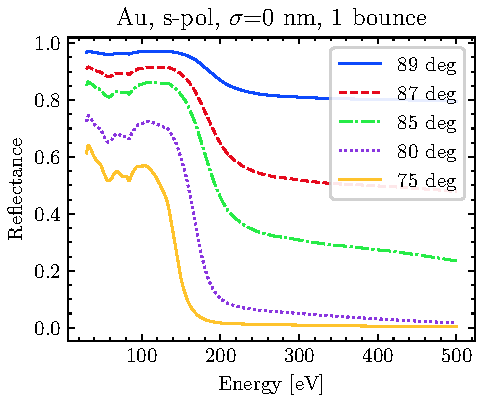
\includegraphics[width=0.75\textwidth]{figures/chap2/Au_ReflvsAngle.pdf}
	\caption{Fresnel reflectance for $s$-polarized light from a single smooth gold mirror as a function of incident angle. Calculation follows \cref{eqn:Fresnel_Rs_1,eqn:DW_2}.}
	\label{fig:Au_ReflvsAngle}
	% generated using Fresnel.py
\end{figure}

\cref{fig:Au_ReflvsAngle} shows the reflectivity of a single gold mirror for various incident angles. As expected, the best performance occurs at small grazing angles. However, for a fixed beam size, the required optic size increases as the grazing angle decreases. The footprint (area) $F$ of a rectangular beam on the optic is given by the geometric projection \cite{gibaudSpecularReflectivitySmooth2009}:
\begin{equation}
F = \frac{t_1}{\cos \theta_i}t_2
\label{eqn:EM_footprint}
\end{equation}
Here, $t_1$ and $t_2$ are the rectangular dimensions of the input beam and $\theta_i$ is the incident angle of the light. If we do not scale the mirror size with the incident angle, we will clip the beam and lose XUV flux. Our desire to have a modular vacuum apparatus with a demagnifying XUV optic is therefore in direct conflict with our desire to have high XUV flux. The exit arm of the mirror, which is proportional to the demagnification factor, must be large enough so that the interaction region can be contained within a separate chamber from the rest of the beamline. We clearly cannot achieve the specifications of a typical x-ray mirror in a synchrotron facility ($\approx 0.5$ degree grazing angle, $\approx 1$ m lateral dimension). Returning to \cref{fig:Au_ReflvsAngle}, we can see that an 87 degree mirror drastically outperforms an 85 degree mirror above 200 eV, but according to \cref{eqn:EM_footprint}, it will be 67\% larger in the horizontal dimension. Larger mirrors have more mass, which increases the requirements for the \textit{in vacuo} motorization, further increasing the cost and required chamber size. Finally, the manufacturing cost and lead time of the mirror is proportional to the polished area. Through an interative design process involving the optical, motorization and vacuum chamber design elements, as well as Zeiss' manufacturing considerations, we decided to use an 85 degree mirror in the TABLe. This allowed us to place the interaction region in a separate chamber, minimized the cost of the mirror, and delivered better than 50\% reflectivity below 200 eV while utilizing small form factor motors and stages. 

\begin{figure}
	\centering
	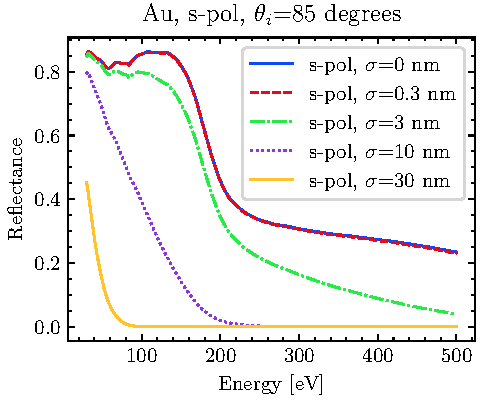
\includegraphics[width=0.75\textwidth]{figures/chap2/R_vs_roughness.pdf}
	\caption{Effect of surface roughness on reflectance. Calculation follows \cref{eqn:Fresnel_Rs_1,eqn:DW_2}.}
	\label{fig:R_vs_roughness}
	% generated using Fresnel.py
\end{figure}

The effect of the surface roughness is shown in \cref{fig:R_vs_roughness}. When polishing glass surfaces, a surface roughness of 0.3 nm is considered state of the art and approaches a height variation of a single atomic layer. Below 500 eV, the difference between a surface with 0.3 nm roughness and an ideal interface is negligible. 

\subsection{Aberration-Free Focusing}

XUV mirrors are typically simple rotational solids (cylinder, toroid, ellipsoid, etc.), and we considered several configurations during the planning stage. It is well known that reflective optics operating at grazing angles can cause abberations at the focus. These abberations introduce phase nonuniformity, smearing the XUV pulse out in time and reducing the effective temporal resolution of the apparatus \cite{bourassin-bouchetHowFocusAttosecond2013}. Additionally, abberations change the shape of the XUV focal spot, which results in a larger range of IR intensities throughout the XUV-IR interaction volume for a fixed IR focusing geometry. Therefore it is critical to minimize or eliminate abberations through optical design.

\subsubsection{The Light Path Function}

\begin{figure}
	\centering
	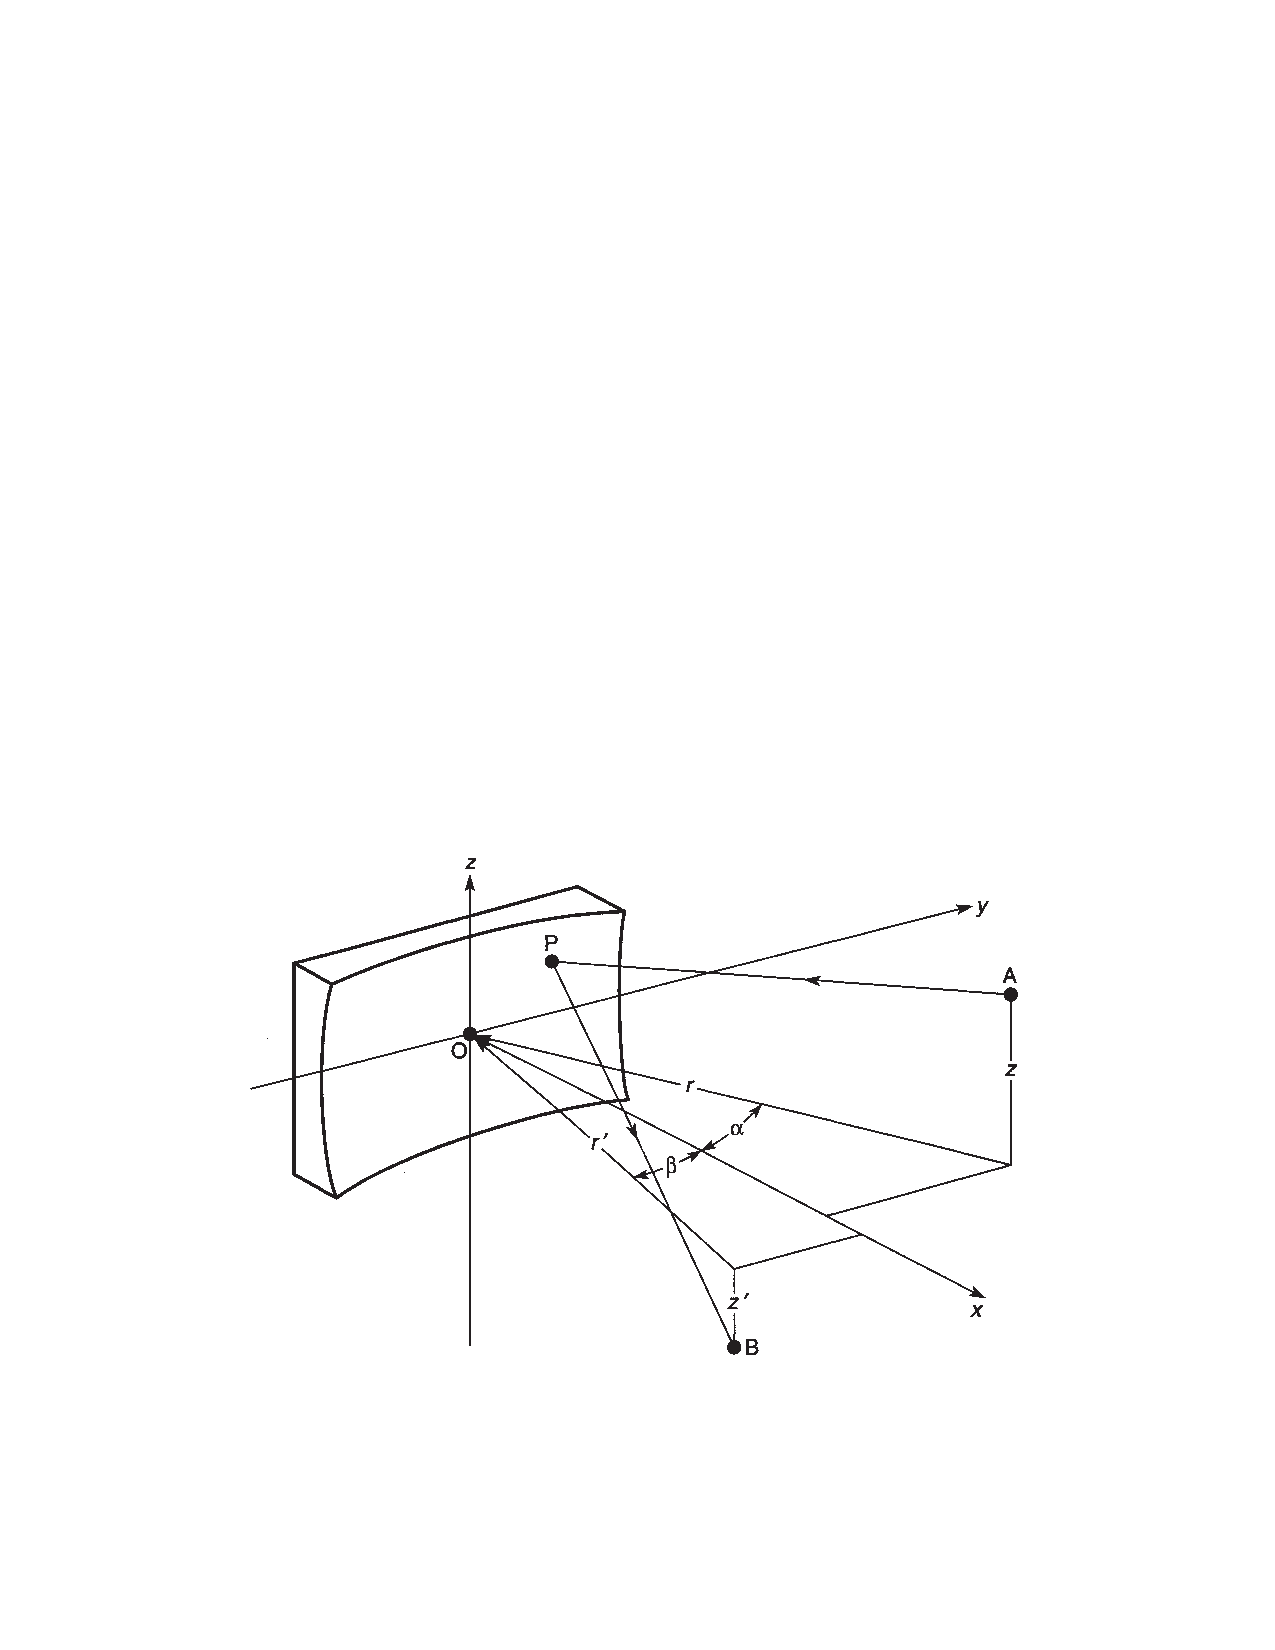
\includegraphics[width=0.75\textwidth]{figures/chap2/LPF_geometry.pdf}
	\caption{Coordinate system used for the light path function $F$. Source point $A$ is located a distance $r$ from the center of the mirror at angle $\alpha$ and height $z$. Focus point $B$ is located a distance $r'$ away, with angle $\beta$ and height $z'$. The impact point $P$ of an individual ray is located on the mirror surface at point $(y,z) = (w,l)$. The curvature of the mirror is used to calculate the distance $x$ between $P(w, l)$ and the $yz$ plane. Figure adapted from \cite{howellsMirrorsSynchrotronRadiationBeamlines1994}.}
	\label{fig:LPF_geometry}
	% snipped from Howell 1994
\end{figure}

Abberations are mathematically analyzed using the \textit{light path function} \cite{nodaGeometricTheoryGrating1974,howellsMirrorsSynchrotronRadiationBeamlines1994,polettoMicrofocusingAttosecondPulses2013}. Consider a reflective optic with an optical surface in the $yz$ plane as shown in \cref{fig:LPF_geometry}. The height of the optic surface $x$ can be described by the following power series:
\begin{equation}
x = \sum_{i=0}^{\infty} \sum_{j=0}^{\infty} a_{ij} y^i z^j, \quad a_{00} = a_{10} = 0, \quad j = \textrm{ even}
\label{eqn:mirror_power_series}
\end{equation}
This expansion can be used to describe spherical, cylindrical, toroidal, ellipsoidal, or other aspheric surfaces given proper values of the coefficients $a_{ij}$.\footnote{Tables 2 and 3 in reference \cite{howellsMirrorsSynchrotronRadiationBeamlines1994} provide $a_{ij}$ values for an ellipsoidal and toroidal mirror, respectively.} Now consider the situation shown in \cref{fig:LPF_geometry}, where a ray is emitted from a point source $A$ and focused at point $B$ after reflecting off the surface of the optic at point $P$. The distance this ray travels is called the light path function, $F = \overline{AP} + \overline{PB}$. 
We are primarily concerned with abberations at the focus which are proportional to the derivative of $F$ with respect to impact coordinates $w$ and $l$. So, we drop the zeroth-order constant $r + r'$ and perform a power series expansion with respect to the impact point $P(w,l)$:
\begin{multline}
F = w F_{100} + w F_{102} + l F_{011} + \frac{1}{2} w^2 F_{200}+ \frac{1}{2} l^2 F_{020} \\
+ \frac{1}{2} w^3 F_{300} + \frac{1}{2} w l^2 F_{120} + w l F_{111} + \frac{1}{8} w^4 F_{400} + \frac{1}{4} w^2 l^2 F_{220} \\
+ \frac{1}{4} w^2 F_{202} + \frac{1}{2} l^2 F_{022} + \frac{1}{2} l^3 F_{031} + \frac{1}{2} w^2 l F_{211} + \cdots
\label{eqn:LPF_Fijk}
\end{multline}
This expression is valid for both mirrors and gratings, but it can be greatly simplified for our application. For a non-holographic grating, the coefficients of $F$ must take the form $F_{ijk} = E_{ijk}(\alpha, r, z) + E_{ijk}(\beta, r', z')$. Next, if points $A$ and $B$ are within the symmetry plane of the mirror ($z=z'=0$), then subscript $k$ must be equal to zero. Finally, from the law of reflection, we have $\alpha = -\beta$. Putting it all together, the coefficients of the series expansion of $F$ have the form:
\begin{equation}
F_{ij0} = E_{ij0}(\alpha, r, 0) + E_{ij0}(-\alpha, r', 0)
\end{equation}

\begin{table}[]
	\centering
	\begin{tabular}{|c|c|c|c|c|c|}
		\hline
		\diagbox{\textbf{i}}{\textbf{j}} & \textbf{0} & \textbf{1} & \textbf{2} & \textbf{3} & \textbf{4} \\ \hline
		\textbf{0} & 0 & 0 & $S$ & 0 & $\frac{4a_{02}^2-S^2}{r} - 8a_{04} \cos \alpha$ \\ \hline
		\textbf{1} & $- \sin \alpha$ & 0 & $\frac{S \sin \alpha}{r} - 2 a_{12} \cos\alpha$ & 0 & * \\ \hline
		\textbf{2} & $T$ & 0 & \makecell{$\frac{4 a_{20} a_{02} - TS -2a_{12} \sin 2 \alpha}{r}$ \\ $+ \frac{2 S \sin^2 \alpha}{r^2} - 4 a_{22} \cos \alpha$} & 0 & * \\ \hline
		\textbf{3} & $\frac{T \sin\alpha}{r} - 2 a_{30} \cos \alpha$ & 0 & * & 0 & * \\ \hline
		\textbf{4} & \makecell{$\frac{4 a_{20}^2 - T^2 - 4a_{30} \sin 2 \alpha}{r}$ \\ $+ \frac{4 T \sin^2 \alpha}{r^2} - 8 a_{40} \cos \alpha$} & 0 & * & 0 & * \\ \hline
	\end{tabular}
	\caption{Values of $E_{ij0}(\alpha, r, 0)$ up to \nth{4} order, used in the calculation of the light path function $F$. Terms in excess of \nth{4} order are indicated by *. See text for definitions of $S$ and $T$. Table adapted from \cite{howellsMirrorsSynchrotronRadiationBeamlines1994}.}
	\label{tab:LPF_Eij0}
\end{table}

The values of $E_{ij0}(\alpha, r, 0)$ can be found in the literature and in \cref{tab:LPF_Eij0}. The terms $S$ and $T$ used in this table are defined below:
\begin{align}
T &= \frac{\cos^2 \alpha}{r} - 2 a_{20} \cos \alpha \\
S &= \frac{1}{r} - 2 a_{02} \cos \alpha
\end{align}
Note that information about the shape of the mirror is connected to the $F_{ij0}$ expansion coefficients via the $a_{ij}$ mirror surface expansion coefficients. Therefore, we can apply this framework to calculate the abberations at the focus for a given mirror shape and geometry.

A consequence of Fermat's Principal of Least Time is that $F$ will be an extrema for any point $P$ on the mirror's surface. Therefore, abberation-free image focusing can be obtained if $\delta F/\delta w = \delta F / \delta l = 0$. This condition must hold for any value of $w$ and $l$ on the mirror's surface, from which it follows that all $F_{ij0}$ terms are identically zero. We can quantify aberrations at the focus using a geometric ray approximation, in which we calculate the displacements of the rays from the image point $B$:
\begin{gather}
\begin{aligned}
\Delta y'_{ij0} &= \frac{r'}{\cos \alpha} \left( \frac{\delta F}{\delta w} \right)_{ij0} \\
\Delta z'_{ij0} &= r' \left( \frac{\delta F}{\delta l} \right)_{ij0}
\end{aligned}
\end{gather}
The total ray abberation in the $\Delta y'$ $(\Delta z')$ direction is the algebraic sum of the above terms for all values of $i$ and $j$. Therefore, the total ray abberation (to \nth{4} order) is:
%\begin{gather}
%\begin{aligned}
%\Delta z' &= r' \left( F_{020} l + F_{120} w l \right) \\
%\Delta y' &= \frac{r'}{\cos \alpha} \left( \frac{1}{2} F_{120} l^2 + F_{200} w + \frac{3}{2} F_{300} w^2 \right)
%\end{aligned}
%\label{eqn:abberation_expansion}
%\end{gather}
\begin{gather}
\begin{aligned}
\Delta y' &= \frac{r'}{\cos \alpha} \left( F_{100} + F_{200} w + \frac{1}{2} F_{120} l^2 + \frac{3}{2} F_{300} w^2  + \frac{1}{2} F_{400} w^3 + \frac{1}{2} F_{220} w l^2 \right) \\
\Delta z' &= r' \left( F_{020} l + F_{120} w l + \frac{1}{2} F_{220} w^2 l + \frac{1}{2} F_{040} l^3 \right)
\end{aligned}
\label{eqn:abberation_expansion}
\end{gather}

We now have expressions for the abberations as a function of the shape of the XUV mirror, which will be applied to different mirror configurations.

\subsubsection{Toroidal Mirrors}

A toroidal mirror is a section of the interior surface formed by a torus (similar to a bicycle tire) described by radii $R$ and $\rho$. There are many advantages to using a toroid in an XUV beamline. Toroidal mirrors operated in a $2f-2f$ configuration can re-image the source point without introducing any aberrations at the focus \cite{chirlaAttosecondPulseGeneration2011}. Additionally, the toroid's constant curvature allows it to be manufactured to a higher degree of accuracy than other shapes \cite{howellsMirrorsSynchrotronRadiationBeamlines1994}. As a result they are very affordable, starting as low as \$5,000.

The toroidal mirror can be designed to reduce abberations. Owing to its symmetry, a toroid naturally has ${F_{100} = F_{120} = 0}$. An analysis of the $F_{ij0}$ expansion coefficients reveals $F_{200}$ and $F_{020}$ will also equal zero if the toroid's radii are set to the following values:
\begin{gather}
\begin{aligned}
\rho &= \frac{2 r r' \cos \alpha}{r + r'} \\
R &= \frac{2 r r' \sec \alpha}{r+r'}
\end{aligned} 
\end{gather}
With these radii, the remaining non-zero terms of \cref{eqn:LPF_Fijk} are $F_{040}, F_{220}, F_{300}$ and $F_{400}$. Introducing the \textit{demagnification factor} $M = r / r'$, the non-zero terms have the following values:
\begin{gather}
\begin{aligned}
F_{300} &= - \left( \frac{M^2-1}{M} \right) \frac{\cos^2 \alpha \sin \alpha}{2 (r')^2} \\
F_{040} &= - \frac{(M^2-1)(M+1)}{M^3 (r')^3} \\
F_{220} &= \frac{2 (M^3+1) - (3M^3 - M^2 - M + 3) \cos 2 \alpha}{4 M^3 (r')^3} \\
%F_{400} &= - \frac{\cos^2 \alpha}{4 M^3 (r')^3} \left[ (-4 + 5 \cos 2 \alpha \right) + (2-\cos 2 \alpha) M + (2 - 3 \cos 2 \alpha) M^2 + ( -4 + 5 \cos 2 \alpha ) M^3 \right] \\
F_{400} &= - \frac{(1+M) \cos^2 \alpha \left[-4 + 6M -4M^2 + (5+M(-8+5M)) \cos 2 \alpha\right]}{4 M^3 (r')^3}
\end{aligned}
\label{eqn:TM_nonzero_Fij0}
\end{gather}
Recalling \cref{eqn:abberation_expansion}, we see that $F_{300}$ corresponds to a second-order aberration, and $F_{040}, F_{220}$ and $F_{400}$ correspond to third-order and fourth-order aberrations. For the special case of $M=1$, \cref{eqn:TM_nonzero_Fij0} simplifies to:
\begin{gather}
\begin{aligned}
F_{300} &= 0 \\
F_{040} &= 0 \\
F_{220} &= \frac{2 \sin^2 \alpha}{(r')^3} \\
F_{400} &= \frac{2 \cos^2 \alpha \sin^2 \alpha}{(r')^3}
\end{aligned}
\end{gather}
So, the toroid only has third-order aberrations if $M=1$, but second-order aberrations exist if $M \ne 1$.

\begin{figure}
	\centering
	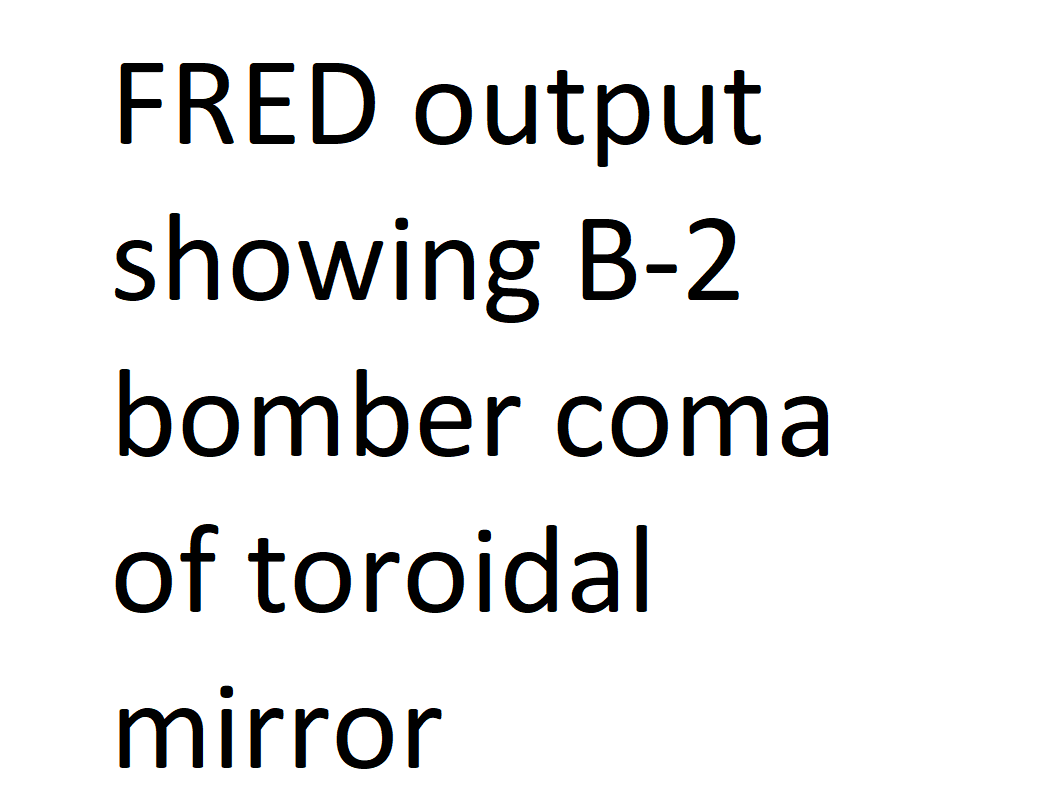
\includegraphics[width=0.75\textwidth]{figures/chap2/TM_coma.png}
	\caption{Complex raytracing simulation showing severe abberations at the focus of a demagnifying toroidal mirror (TM). The entrance arm $l_1$ is 150 cm, the exit arm $l_2$ is 50 cm, and the grazing angle is 5 degrees. Top panel: overhead view of the simulation showing the source rays (red) and the focused rays (green). Bottom panel: intensity at the focal plane in arbitrary units. Calculations were performed using Photon Engineering's FRED software \cite{pfistererFREDOpticalEngineering}.}
	\label{fig:TM_coma}
\end{figure}

Simulations of a demagnifying ($M=3$) toroidal mirror were performed using numerical complex ray tracing techniques, implemented via Photon Engineering's FRED software \cite{pfistererFREDOpticalEngineering,arnaudRepresentationGaussianBeams1985}. The results of this simulation are shown in \cref{fig:TM_coma}. We can see strong abberations are present at the focus that would be detrimental to the performance of the TABLe apparatus. For this reason, we decided against using a toroid in our beamline.

\subsubsection{Spherical Mirrors}

It is well known that spherical mirrors introduce significant aberration when operated away from normal incidence \cite{howellsMirrorsSynchrotronRadiationBeamlines1994}. This is because a spherical mirror is simply a toroidal mirror with equal radii of curvature ($R=\rho$). For this reason, we did not pursue a spherical mirror solution.

\subsubsection{Dual Mirror Configurations}

Introducing a second XUV optic can counteract the abberations introduced by the first \cite{howellsMirrorsSynchrotronRadiationBeamlines1994}. The most common configuration is the Kirtpatrick-Baez (KB) mirror pair, which is commonly used in synchrotrons \cite{kirkpatrickFormationOpticalImages1948}. A KB mirror pair consists of two cylindrical mirrors with the normal direction of their optical surfaces placed orthogonally to each other and the beam propagation direction. In this geometry, each mirror focuses along one direction, and together they act as a single optic that focuses in both transverse directions. Another option is a dual toroid configuration, which has a real focus located between the two mirrors \cite{polettoMicrofocusingAttosecondPulses2013}. Both of these ideas were considered but ultimately deemed impractical.

\begin{figure}
	\centering
	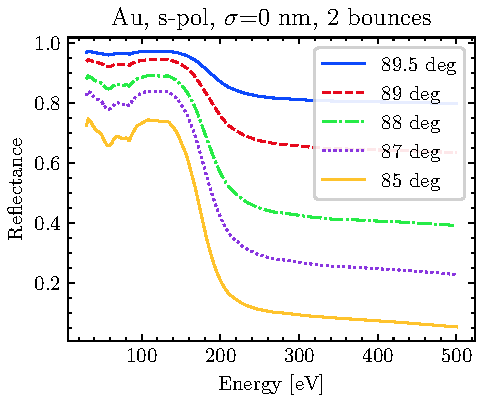
\includegraphics[width=0.75\textwidth]{figures/chap2/Au_ReflvsAngle_2bounce.pdf}
	\caption{Fresnel reflectance for $s$-polarized light from two smooth gold mirrors as a function of incident angle. Calculation follows \cref{eqn:Fresnel_Rs_1,eqn:DW_2}.}
	\label{fig:Au_ReflvsAngle_2bounce}
	% generated using Fresnel.py
\end{figure}

\cref{fig:Au_ReflvsAngle_2bounce} illustrates the problem with a dual optic design design. Two 85 degree optics have a reflectance of only 20\% at 200 eV, and have at least twice the footprint as a single 85 degree optic. To achieve the performance of a single 85 degree optic at 200 eV, the mirror pair needs to be operated at 87 degrees. As discussed above, this 87 degree pair will be 3.33 times larger than a single 85 degree optic in the beam propagation direction. On the other hand, if we want our two mirror configuration to maintain the footprint of a single 85 degree optic, it needs to be operated at 80 degrees. This geometry yields a reflectivity of only 1\% at 200 eV, which is insufficient for our experimental requirements. Clearly, a single-optic solution is preferrable.

\subsubsection{Ellipsoidal Mirrors}

We can apply the same light path function analysis to the ellipsoidal mirror. If we do the analysis, we will see that most of the terms in \cref{eqn:LPF_Fijk} are identically zero. The only non-zero term is $F_{220}$, which evaluates to:
\begin{equation}
F_{220} = \frac{(1+M) \left[-3-M(2+3M)+3(M-1)^2 \cos 2 \alpha \right] (\cot \alpha + \tan \alpha -2)}{16 M^3 (r')^3}
\end{equation}
As a result, the light path function for an ellipsoid is simply $F = \frac{1}{4} w^2 l^2 F_{220}$. Therefore, the largest abberations from an ellipsoid are third-order in the abberation expansion, which is a significant improvement upon the performance of a toroidal mirror.

We have shown that an ellipsoidal mirror is able to demagnify a point source without introducing significant abberations at the focus. As a single optic solution, it avoids the reflectivity losses of a dual mirror configuration. However, its variable radius of curvature provides manufacturing challenges that have only been overcome in the past several years \cite{motoyamaErrorAnalysisEllipsoidal2014}. This requires the use of special manufacturing techniques thats significantly raise the cost and lead time of the optic. At the time of purchase, Carl Zeiss Laser Optics GmbH was the only company that could manufacture and verify the shape of an ellipsoidal mirror that met our technical requirements.

The shape of the rotational ellipsoid can be completely described by three parameters: the two semiaxes ($a$, $b$) and the horizontal\footnote{Our mirror has vertical symmetry, so $y_M=0$.} off-axis position $y_M$. An alternative set of parameters are the entrance and exit arm lengths ($l_1$, $l_2$) and the grazing angle $\alpha$. Additionally, the spatial extent (clear aperture) of the optic is specified by the tangential length $L$ and the out-of-plane width $W$. Below, we will show how these quantities are related.

In a Cartesian coordinate system, an ellipsoid of revolution is described by parameters $a$ and $b$:
\begin{equation}
\frac{x^2}{a^2} + \frac{y^2 + z^2}{b^2} = 1
\end{equation}
where the $xy$ plane is the (horizontal) optical plane and $z$ is the direction orthogonal to the optical plane (vertical).\footnote{Note that this coordinate system differs from the one used to describe the mirror surface in the previous section.} Due to the symmetry between $y$ and $z$, much of the analysis can be done in the optical plane ($z=0$):
\begin{equation}
\frac{x^2}{a^2} + \frac{y^2}{b^2} = 1
\label{eqn:ellipse}
\end{equation}

\begin{figure}
	\centering
	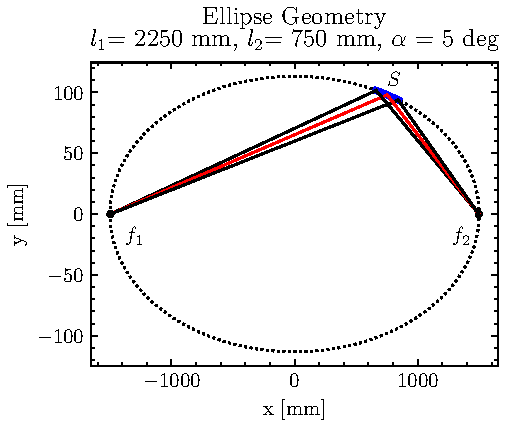
\includegraphics[width=0.75\textwidth]{figures/chap2/EM_2D.pdf}
	\caption{Overhead view of the ellipsoidal mirror geometry used in our beamline. Mirror surface $S$ is shown in blue; foci $f_{1,2}$ are represented by black dots. Rays that strike the center (red) and the edges (black) of the mirror are depicted as lines. Vertical scale is enlarged to show detail. Drawing is otherwise to scale to match the dimensions in \cref{tab:EM_specs}.}
	\label{fig:EM_2D}
	% figure made in EM_geometry.py
\end{figure}

In the $xy$ plane, the surface of the mirror is a segment of the curve formed by \cref{eqn:ellipse}, which is shown in \cref{fig:EM_2D}. The center of the mirror (off-axis position) is denoted by $(x,y)=(x_M, y_M)$. The ellipse has eccentricity $\epsilon$,
\begin{equation}
\epsilon = \sqrt{1-\frac{b^2}{a^2} } \text{,}
\end{equation}
and focal points at positions $(x,y) = (\pm a \epsilon,0)$. Consider a light source at the first focal point,  $f_1 = (-a \epsilon,0)$: rays emanating from $f_1$ will strike surface of the ellipse at some point $S = (x_0, y_0)$ and focus to $f_2 = (a \epsilon,0)$. This optical system has an entrance arm $l_1 = f_1S$, exit arm $l_2=Sf_1$, and demagnification $M$ given by:
\begin{align}
l_1 &= \sqrt{ (x_0+a \epsilon)^2 + y_0^2 } \\
l_2 &= \sqrt{ (x_0-a \epsilon)^2 + y_0^2 } \\
M &= \frac{l_1}{l_2}
\end{align}
Once the $f_1$, $f_2$ and $S$ are defined, the grazing angle $\alpha$ of reflection can be found by applying the Law of Cosines:
\begin{equation}
\alpha = \frac{1}{2} \arccos \left( \frac{(2 a \epsilon)^2 - l_1^2 - l_2^2}{2 l_1 l_2} \right)
\end{equation}

\subsubsection{Our Ellipsoidal Mirror}

\begin{table}[]
	\begin{tabular}{|llll|}
		\hline
		\textbf{substrate} &  &  &  \\
		surface geometry & concave rot. ellipsoid &  &  \\
		material & fused Silica HOQ310 &  &  \\
		dimensions ($L \times W \times H$) & $240 \times 76 \times 45 \pm 0.2$ mm &  &  \\ \hline
		\textbf{optical surface} &  &  &  \\
		clear aperture ($L \times W$) & $180 \times 16$ mm &  &  \\
		footprint geometry & rectangular &  &  \\ \hline
		\multicolumn{2}{|l|}{\textbf{geometry parameters}} & \multicolumn{2}{l|}{\textbf{alternative set}} \\
		semiaxis $a$ & \multicolumn{1}{l|}{1500 mm} & entrance arm $l_1$ & 2250 mm \\
		semiaxis $b$ & \multicolumn{1}{l|}{113.219 mm} & exit arm $l_2$ & 750 mm \\
		off-axis position $x_M$ & \multicolumn{1}{l|}{752.146 mm} & grazing angle & 5 deg \\ \hline
		\multicolumn{2}{|l|}{\textbf{surface quality}} & \textbf{spatial sampling rate} &  \\
		tangential slope error & \multicolumn{1}{l|}{$\le 2.0$ arcsec (rms)} & $2 - 180$ mm &  \\
		sagittal slope error & \multicolumn{1}{l|}{$\le 10.0$ arcsec (rms)} & $2 - 16$ mm &  \\
		mid spatial frequency roughness & \multicolumn{1}{l|}{$\le 0.3$ nm (rms)} & $1.0 - 200 \textrm{ } \mu$m &  \\ \hline
		\textbf{coating material} &  &  &  \\
		$40 \pm 5$ nm Au w/ Cr binding layer &  &  &  \\ \hline
	\end{tabular}
	\caption{Specifications of the ellipsoidal mirror. Data provided by Carl Zeiss Laser Optics GmbH.}
	\label{tab:EM_specs}
\end{table}

We used the results of the previous sections to specify the parameters of our XUV mirror, which can be found in \cref{tab:EM_specs}. A picture of the mirror can be seen in \cref{fig:EM_in_mount}. A rotational ellipsoid was chosen for its aberration-free focusing when used in a demagnifying geometry. A demagnification factor of $M = 3$ and a grazing angle of 5 degrees were chosen because they represent a compromise between our optical requirements of high flux at high photon energies and the mechanical limitations of a modular beamline. When performing ATAS experiments, this demagnification factor gives us a $\simeq 50\%$ signal improvement compared to a 1-to-1 geometry (see \cref{sec:micro_macro_DeltaA} for details). The exit arm was set to be as short as possible while keeping the mirror and target chambers separate, which resulted in an exit arm of 750 mm. A substrate with a 0.3 nm microroughness and a gold coating delivers excellent reflectivity out to 300 eV.

The clear aperture was chosen to match the expected footprint of the harmonics on the optic divergence of the harmonics, which we assumed would have a half-angle divergence of 3.5 mrad. This resulted in a polished region of size $180 \times 16$ mm with an rms roughness of 0.3 nm. A 30 mm border region surrounds this area with a moderately high polish. Zeiss estimates that the surface roughness smoothly increases from the specified 0.3 nm at the edge of the clear aperture to 3 nm at the edge of the substrate.

\begin{figure}
	\centering
	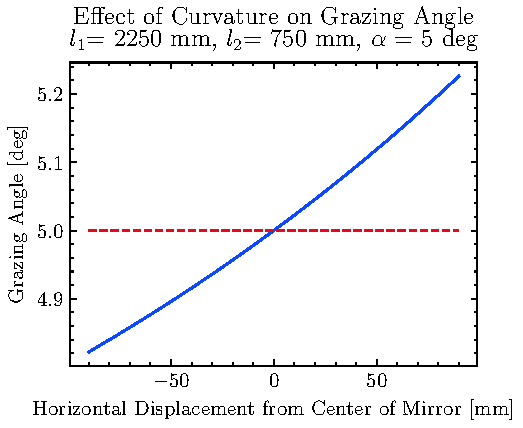
\includegraphics[width=0.75\textwidth]{figures/chap2/EM_angle.pdf}
	\caption{The effect of curvature on the local grazing angle along the mirror's symmetry axis ($z=0$). Light that strikes the edges of the mirror will experience a slightly different grazing angle than the design angle.}
	\label{fig:EM_angle}
	% figure made in EM_geometry.py
\end{figure}

\begin{figure}
	\centering
	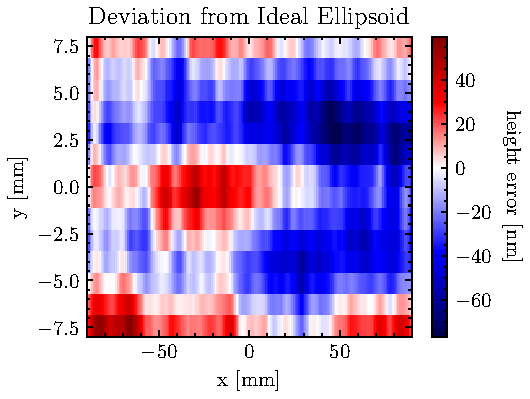
\includegraphics[width=0.75\textwidth]{figures/chap2/EM_error.pdf}
	\caption{Height deviation of our ellipsoidal mirror from an ideal surface, as measured by a Carl Zeiss M400 precision tactile measurement device. Data provided by Carl Zeiss Laser Optics GmbH.}
	\label{fig:EM_error}
	% figure made in \Python Scripts\CXRO\EM_geometry.py
	% data obtained from private communication with Norman Niewrzella of Zeiss. 
\end{figure}

The finite spatial extent of a physical mirror will result in a range of grazing angles across its surface, as shown in \cref{fig:EM_angle}. For our mirror, the grazing angle ranges from 4.8 to 5.25 degrees, which does not significantly change the reflectance shown in \cref{fig:Au_ReflvsAngle}. Finally, the spatially resolved height error is shown in \cref{fig:EM_error}, which shows the excellent manufacturing tolerances of our mirror's surface.

\subsection{Metallic Filters}

\begin{figure}
	\centering
	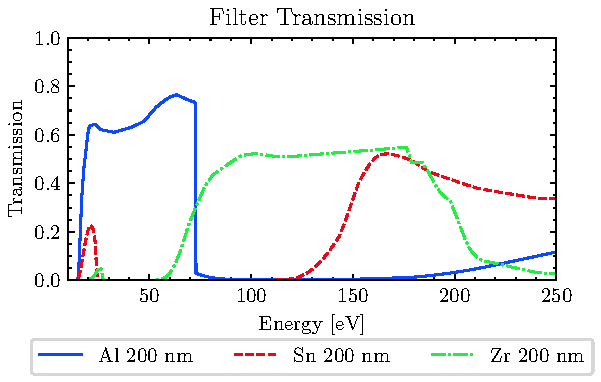
\includegraphics[width=0.75\textwidth]{figures/chap2/Filter_transmission_CXRO.pdf}
	\caption{Calculated XUV transmission of various metallic filters. Data from \cite{gulliksonCXROXRayInteractions}.}
	\label{fig:Filter_transmission_CXRO}
	% figure generated using \PythonScripts\CXRO\test\CXRO.py
\end{figure}

We use a thin metallic filter to block the infrared field after the HHG process (located in chamber $F_1$ in \cref{fig:TABLE_overhead_drawing}). The XUV transmission of the most commonly used filters is shown in \cref{fig:Filter_transmission_CXRO}. Aluminum is favored for experiments below 100 eV, zirconium is useful between 70 and 160 eV, and tin is best suited above 160 eV. 

\section{IR Optics}
Next, we discuss the infrared optics used in the generation and pump arms. This includes the optics used for generating harmonics in the generation arm; in the pump arm we have the pulse energy and delay control optics and the focusing optics. We also have the beam splitter and the hole mirror, which mark the beginning and end of the interferometer, respectively.

We wanted the infrared optics to be as achromatic as possible, which would allow us to perform wavelength scans using the TOPAS, or to switch from the signal to the idler or the depeted 800 nm pump without having to completely rebuild the interferometer. Additionally, we wanted the ability to easily access the pump arm's optics, which meant keeping the pump arm out of vacuum until right before recombination with the XUV arm. This has the extra benefit of allowing future exotic upgrades to the pump arm, such as THz generation, DFG, SHG, etc. With the exception of the hole mirror, all IR optics are outside the vacuum system. 

\subsection{The Generation Arm}

We use 2" diameter silver optics throughout the beamline unless otherwise specified. As a future upgrade, we purchased high reflectivity dielectric mirrors (Lambda Optics BHR-5012B-1200-1600-45U, coated for $\lambda = 1.2 - 1.6$ $\mu$m) for use with the signal wavelengths.

The generation arm takes the transmitted light from a 4/96\% beamsplitter (BS, Thorlabs UVFS BSF20-C). A telescope (L1, $f = - 300$ mm; L2, $f = + 500$ mm) enlarges the beam, allowing for tighter focusing in the generation chamber, which is useful when operating at longer wavelengths. A focusing lens (L3, $f= 400$ mm) and an adjustable aperture (iris) are located immediately before a CaF\textsubscript{2} window (3 mm thick) on the entrance flange of the generation chamber. The distance between the outer surface of the CaF\textsubscript{2} window and the center of the chamber is 23.8 cm. This geometry supports focal lengths 30 cm or longer outside the chamber. It is possible to mount shorter focal length optics inside the generation chamber using the internal breadboard. There is enough room outside the chamber to implement an $f = 40$ cm reflective focusing setup, but reflective setups using shorter focal lengths will require in-vacuum optics or modifications to the chamber. A metallic filter blocks the IR light about 1 meter after the IR focus (chamber $F_1$ in \cref{fig:TABLE_overhead_drawing}).

A computer controlled home-built shutter (S in \cref{fig:beamline_schematic}) is located before telescope. This shutter is used to block the laser, which is useful when performing certain operatings (finding overlap, moving the sample holder in the target chamber, manipulating the filter assembly, etc.).

For experiments that require additional harmonic bandwidth, we insert additional optics (a BBO crystal, 200 $\mu$m of calcite, and a zero-order 1310 nm $\lambda/2$ waveplate) between $L3$ and the vacuum window. When aligned correctly, these optics create a spatially and temporally overlapped $\omega$ and $2\omega$ fields at the focus.

\subsection{The Pump Arm}

The pump arm takes the reflected light (4\%) from the beamsplitter and propagates in air on the upper deck of the split-level optical table.

A 1 $\mu$m longpass filter (Thorlabs FELH1000, $\text{OD}>5$) is positioned before the waveplate-polarizer assembly to filter out the OPA's visible parasitic wavelengths. This is neccessary to suppress short-wavelength excitation of condensed matter samples. The IR intensity incident on the sample is controlled by a motorized achromatic $\lambda/2$ waveplate (Thorlabs AHWP10M-1600, $\lambda = 1100 - 2000$ nm) and a pair of ultra broadband wire grid polarizers (Thorlabs WB25M-UB, each with a 1000:1 extinction ratio for $\lambda = 0.6 - 4 \ \mu \text{m}$) in the pump arm (see \cref{fig:beamline_schematic}). 

The XUV-IR delay is coarsely adjusted using a retroreflector on a manual translation stage, with $\Delta \tau = 2 \Delta x / c =  6.67 \ \left[ \textrm{fs}/ \mu \textrm{m} \right] \Delta x$. Motorizing this retroreflector could enable the study of ps-scale dynamics. Fine delay control is achieved by sending the laser through a pair of fused silica (Infrasil) opposing wedges. The insertion amount of one wedge into the beam path is controlled by a stepper motor, while the other wedge is fixed in place. Inserting the wedge by an amount $\Delta x$ increases the thickness of glass in the beam path, delaying the pump arm by an amount $\Delta \tau$ \cite{hagemanComplexAttosecondTransientAbsorption2020}:
\begin{equation}
\Delta \tau = \frac{\Delta x}{c} \left[ n \tan \theta - \frac{\sin \theta}{\cos \varphi} - n \tan \theta \left( \frac{\sin \left(\varphi - \theta \right)}{\cos \theta}\right) \right]
\label{eqn:wedge_delay}
\end{equation}
where $n$ is the refractive index of the wedge material, $\theta$ is the wedge angle and ${\varphi \equiv \arcsin \left( n \sin \theta \right)}$ is calculated from Snell's law. For $\lambda = 1430 \ \textrm{nm}$ and $\theta = 4.5 \ \textrm{degrees}$, $n=1.4454$ \cite{malitsonInterspecimenComparisonRefractive1965} and \cref{eqn:wedge_delay} evaluates to:
\begin{equation}
\Delta \tau = \left( 102 \left[ \frac{\textrm{as}}{\mu \textrm{m}}\right]\right) \Delta x
\end{equation}
A translation range of $\Delta x = 14 \ \textrm{mm}$ provides a delay range of $\Delta \tau =  1.4 \ \textrm{ps}$.

During an experiment, the intensity is measured using an InGaAs photodiode (Thorlabs DET10D) mounted with a 2.0 absorptive neutral density filter and 1 $\mu$m longpass filter (Thorlabs FELH1000), which detects light scattered off a mirror in the pump arm and is monitored using an oscilliscope (LeCroy). Absolute measurements of the average IR power are taken with a power meter (Gentek) located before the diverging lens L4. A computer controlled home-built shutter S is located after the photodiode so that the intensity can be adjusted while the pump arm is blocked.

We use a pair of AR-coated N-BK7 lenses ($\lambda = 1050-1700$ nm) in the pump arm to minimize the losses from the hole mirror. Diverging lens L4 (Thorlabs LF1015-C, $f = - 300$ mm) expands the beam and converging lens L5 (Thorlabs LA1380-C, $f = + 500$ mm, located 68.5 cm after L4) focuses it into the target chamber. After L5, the IR beam passes through a 3 mm thick CaF\textsubscript{2} window to enter the mirror chamber.

The two arms of the interferometer are combined using a hole mirror (HM), located 53 cm after L5 and 20 cm after the ellipsoidal mirror. The hole mirror is a 2" diameter silver mirror with a 10 mm diameter aperture in the center \cite{peatrossHighorderHarmonicGeneration1994}. The XUV light passes through the aperture from the backside of the mirror, and the IR light reflects off the annular disk on the front face. This geometry allows us to have a collinear XUV-IR geometry without having to resort to bandwidth limiting XUV-IR optics. However, this geometry clips the center of the IR beam and is responsible for IR diffraction at the focus.

\subsubsection{Calculation of IR intensity at Focus}
\label{sec:Pump_Arm_Focus_Calculations}

\begin{figure}
	\centering
	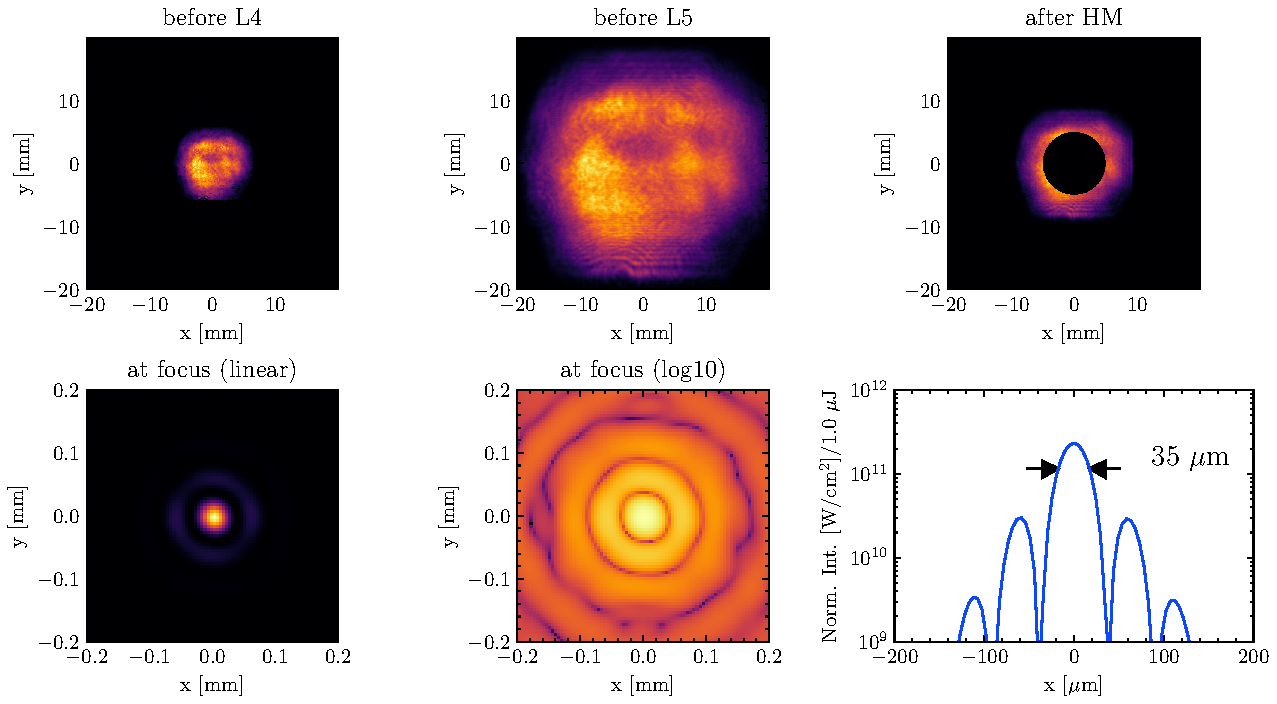
\includegraphics[width=0.9\textwidth]{figures/chap2/pump_on_focus_calculation_8192_inferno.pdf}
	\caption{Numerical propagation of the IR ($\lambda$=1500 nm) beam through the pump arm. Beam path layout follows \cref{fig:beamline_schematic}. Each panel shows the intensity of the beam as the beam propagates towards the focus. The first panel shows the measured intensity (Electrophysics PV320 thermal camera), all other panels are calculations. The arrows on the lineout indicate the FWHM. All calculations are for vacuum ($n=1$).}
	\label{fig:pump_on_focus_calculation}
	% plot made with \Python Scripts\LightPipes\pump_intensity.py using N=2**13 gridside
\end{figure}

The spatial intensity profile $I_0(x,t)$ of the $\lambda$=1500 nm TOPAS pulse was measured immediately before the pump arm's diverging lens (L4 in \cref{fig:beamline_schematic}) using an Electrophysics PV320 thermal camera. We numerically calculated the transverse profile of the IR pulse at the focus $I_{\textrm{diff.}}(x,y)$ by successively applying several operators to $I_0(x,t)$:
\begin{equation}
\begin{aligned}
I_{\textrm{diff.}}(x,y) &= \vb{M} I_0(x,y), \\
\textrm{with} \ \vb{M} &\equiv \vb{L^+}(d_{\textrm{focus}}) \vb{A}_{\textrm{HM}} \vb{L^+}(d_{HM}) \vb*{\tau}(f_5) \vb{L^+}(d_{4,5}) \vb*{\tau}(f_4),
\end{aligned}
\label{eqn:IR_transverse_int_profile}
\end{equation}
In the above, $\vb{L^+}(d)$ is the free-space propagation operator for distance $d$ under the Fresnel approximation evaluated using an FFT method, $\vb*{\tau}_f$ is the complex transmittance of a lens of focal length $f$ (see \cref{eqn:complex_transmittance_lens}), and $\vb{A}$ is a spatially-dependent amplitude mask. This calculation was performed using the Python package \textit{Lightpipes for Python} \cite{vdovinLightPipesPython} using a grid size of $2^{13}\times2^{13}$, and the result is shown in \cref{fig:pump_on_focus_calculation}. Clear apertures of 22.86 mm (L4), 45.72 mm (L5) and 50.8 mm (HM) were used for this calculation. The focal lengths were $f_4 = -300 \ \textrm{mm}$, $f_5 = + 500 \ \textrm{mm}$ and the distances were $d_{4,5} = 68.5 \ \textrm{cm}$, $d_{\textrm{HM}} = 53 \ \textrm{cm}$, $d_{\textrm{focus}} = 48.63 \ \textrm{cm}$. The input profile $I_0(x,y)$ was assumed to have 1 $\mu$J of energy and a 65 fs Gaussian temporal profile.


%\begin{equation}
%\begin{aligned}
%H &= \frac{A(\alpha, \beta, z)}{A(\alpha, \beta, 0)} = \exp \left[ -i k z \sqrt{1 - \alpha^2 - \beta^2} \right] \\
%A(\alpha, \beta, 0) &= \int_{-\infty}^{\infty} \dd{x} \int_{-\infty}^{\infty} \dd{y} U(x,y,0) \exp\left[ -i k z (\alpha x + \beta y) \right] \\
%A(\alpha, \beta, z) &= \int_{-\infty}^{\infty} \dd{x} \int_{-\infty}^{\infty} \dd{y} U(x,y,z) \exp\left[ -i k z (\alpha x + \beta y) \right] \\
%\end{aligned}
%\end{equation}

Reflection losses from 2 Ag mirrors, 2 AR-coated lenses and uncoated $\text{CaF}_2$ vacuum window are responsible for a 26.2\% reduction in transmitted power. Additionally, the geometry of the hole mirror causes only 56\% of incident power to be incident on a reflective surface (the rest is lost to the central aperture). In total, the pump arm transmits 41.3\% of the power from before L4 to the focus.

The IR intensity makes an Airy-like diffraction pattern at the focal plane. There is an intense bright spot surrounded by a series of rings, with the intensity of each ring decreasing as the distance from the center increases. The rings exhibit a periodic modulation in intensity with respect to angle $\phi$. This four-fold symmetry is due to the square-like spatial profile of the TOPAS output, whereas the clipping from the hole mirror's aperture is responsible for the central peak and ring structure. The central lobe has a peak intensity of $\sim 2.3 \times 10^{11} \text{ W/cm}^2$ per 1 $\mu$J input pulse energy and a FWHM of 35 $\mu$m. The first ring has a radius of 59 $\mu$m and a peak intensity $\sim 2.9 \times 10^{10} \text{ W/cm}^2$ per input $\mu$J pulse energy. Thus the central lobe's peak intensity is about an order of magnitude larger than the ring's intensity. However, the central spot only contains about 49\% of the total power, as the rings cover a much larger area.

Note that the above calculations assume perfect alignment into the hole mirror (i.e., the IR beam is centered on the central aperture of the hole mirror). If the IR beam is misaligned to the hole mirror, then the transmission to the focus will increase as the most intense part of the beam is no longer clipped by the central aperture. Therefore, a drift in the laser's pointing during an experiment can effect the sample's interaction intensity.

\subsection{Aligning into the TABLe Interferometer}

We use an Electrophysics PV320 thermal camera for daily alignment into the TABLe interferometer.\footnote{Special thanks to Eric Moore who wrote a LabVIEW program to semi-automate this process.} The camera is located between S and L4, and we use two irises (the \nth{1} is located between BS and CF, the \nth{2} is located just before S) to define the aligned beam path. Two motorized mirror mounts located on the TOPAS table control the pointing of the input beam. The beam is considered to be aligned when the Airy rings from the partially closed \nth{1} iris are centered on the \nth{2} iris, and when the centroid of the beam is centered on the \nth{2} iris. Alignment is achieved by iteratively correcting the beam pointing while checking these two metrics.

\section{XUV Photon Spectrometer}
\label{sec:XUV_spectrometer}

\subsection{Optical Description}

Below is a brief overview of the XUV photon spectrometer's optics. For a complete description, see \cite{hagemanComplexAttosecondTransientAbsorption2020}.

The XUV spectrometer utilizes one of two available concave variable line spaced (VLS) Hitachi gratings, depending on the desired spectral range. Owing to their small grazing angles (1200 lines/mm: 3 deg, 2400 lines/mm: 1.3 deg), they spectrally disperse the light in the horizontal plane while maintaining the vertical spatial profile. The groove spacing is engineered to a flat field across a wide spectral range (1200 lines/mm: 5 - 20 nm, 2400 lines/mm: 1-5 nm). Outside this spectral range, the gratings continue to disperse the light but the focal plane is no longer within the specified flat field. By adjusting the incident angle, we can control both the entrance arm and the flat field spectral range.

The dispersed light hits a 75 mm diameter imaging microchannel plate array (MCP, Photonis) which converts the XUV photons into an electron shower via an avalance process \cite{ladislaswizaMicrochannelPlateDetectors1979a,fraserGrayImagingUsing1984}. A type P47 phosphor screen (P, Photonis) converts the spatially-resolved electron shower into light (370 - 480 nm range, peaked at 400 nm), which is sent outside the chamber via a glass window. The MCP-P assembly is mounted directly to an 8" flange, which is connected to the chamber via an edge welded bellows. An external mechanical assembly controls the angle and position of the detector array relative to the grating. The detector position is adjusted in conjunction with the grating's incident angle to make the flat field coincident with the detector plane for a given spectral range.

A computer-controlled digital 16-bit CMOS camera (Andor Neo DC-152Q-C00-FI) is equipped with a Rodagon 50 mm lens and modular focus (QI Optiq) to image the output light of the phosphor. The camera image is recorded to the TABLe computer's hard drive. The camera images have a maximum resolution of $2560 \times 2160$ (6.5 $\mu$m pixel size) with a sensor size of $16.6 \times 14.0$ mm.

%\textbf{energy resolution of ?, spatial resolution of ??}

\subsection{Spectral Calibration}
\label{sec:XUV-spectral-calibration}

The photon spectrometer measures XUV counts as a function of position along the camera sensor (i.e., in the spectral pixel basis $p$). Owing to the grating equation, the position in the spectral pixel basis is proportional to the photon wavelength $\lambda$ and inversely proportional to the photon energy $E$. However, the position of the detector relative to the grating (set by the cage \& crank and the grating's piezo motors) introduces geometric factors which shift and skew the position of the light on the sensor. It is not practical to measure the exact distances between these two elements, so we perform a numerical fit.

Generally speaking, we calibrate the spectrometer by assigning energies $E_i$ to known spectral features in the data located at spectral pixel $p_i$. These features can be absorption features, resonances, or the harmonics themselves. This yields a set of coordinate pairs $\{(p_i,E_i)\}$ that can be fit to a polynomial $E(p)$. Below, we will discuss the methods used to create these coordinate pairs.

\subsubsection{One-Source Harmonic Counting Scheme}

The most prominent spectral features on the detector are the harmonics themselves. If we have more than an octave of XUV bandwidth, then we can exploit the grating equation and the regular spacing of the harmonics to determine the harmonic order of every harmonic on the detector. Below, we will explain this process.

First, consider the grating equation:
\begin{equation}
d (\sin \theta_i - \sin \theta_m) = m \lambda
\label{eqn:grating-equation}
\end{equation}
where $\theta_i$ is the incident angle, $\theta_m$ is the diffraction angle, $m$ is the diffraction order, and $\lambda$ is the photon wavelength. Inspection of \cref{eqn:grating-equation} reveals that a light of a particular wavelength will appear at multiple locations on the detector, corresponding to each diffraction order ($m=1, 2, 3, \dots$). The grating is designed to deliver most of the light to the \nth{1} order, but an appreciable amount of energy winds up in the \nth{2} and \nth{3} orders \cite{obryanHighResolutionXUV2015,hagemanComplexAttosecondTransientAbsorption2020}.

We will assume that over the spectral region of interest, the wavelength of the $i^{th}$ harmonic is $\lambda_i = \lambda_1 / i$, where $\lambda_1$ is the effective fundamental wavelength. That is, we assume that all of the harmonics on the detector have the same fundamental wavelength and are evenly spaced in energy. Furthermore, we will assume that only odd-order harmonics are present during the calibration step.

As a result of the equal harmonic spacing and having more than an octave of XUV bandwidth, there will be regions of the detector that have light from both \nth{1} and \nth{2} order diffraction. From the grating equation, a \nth{1} order diffraction of the $i^{th}$ harmonic will coincide with the \nth{2} order diffraction of the $(2i)^{th}$ harmonic. This is shown in \cref{fig:harmonic_counting}.

\begin{figure}
	\centering
	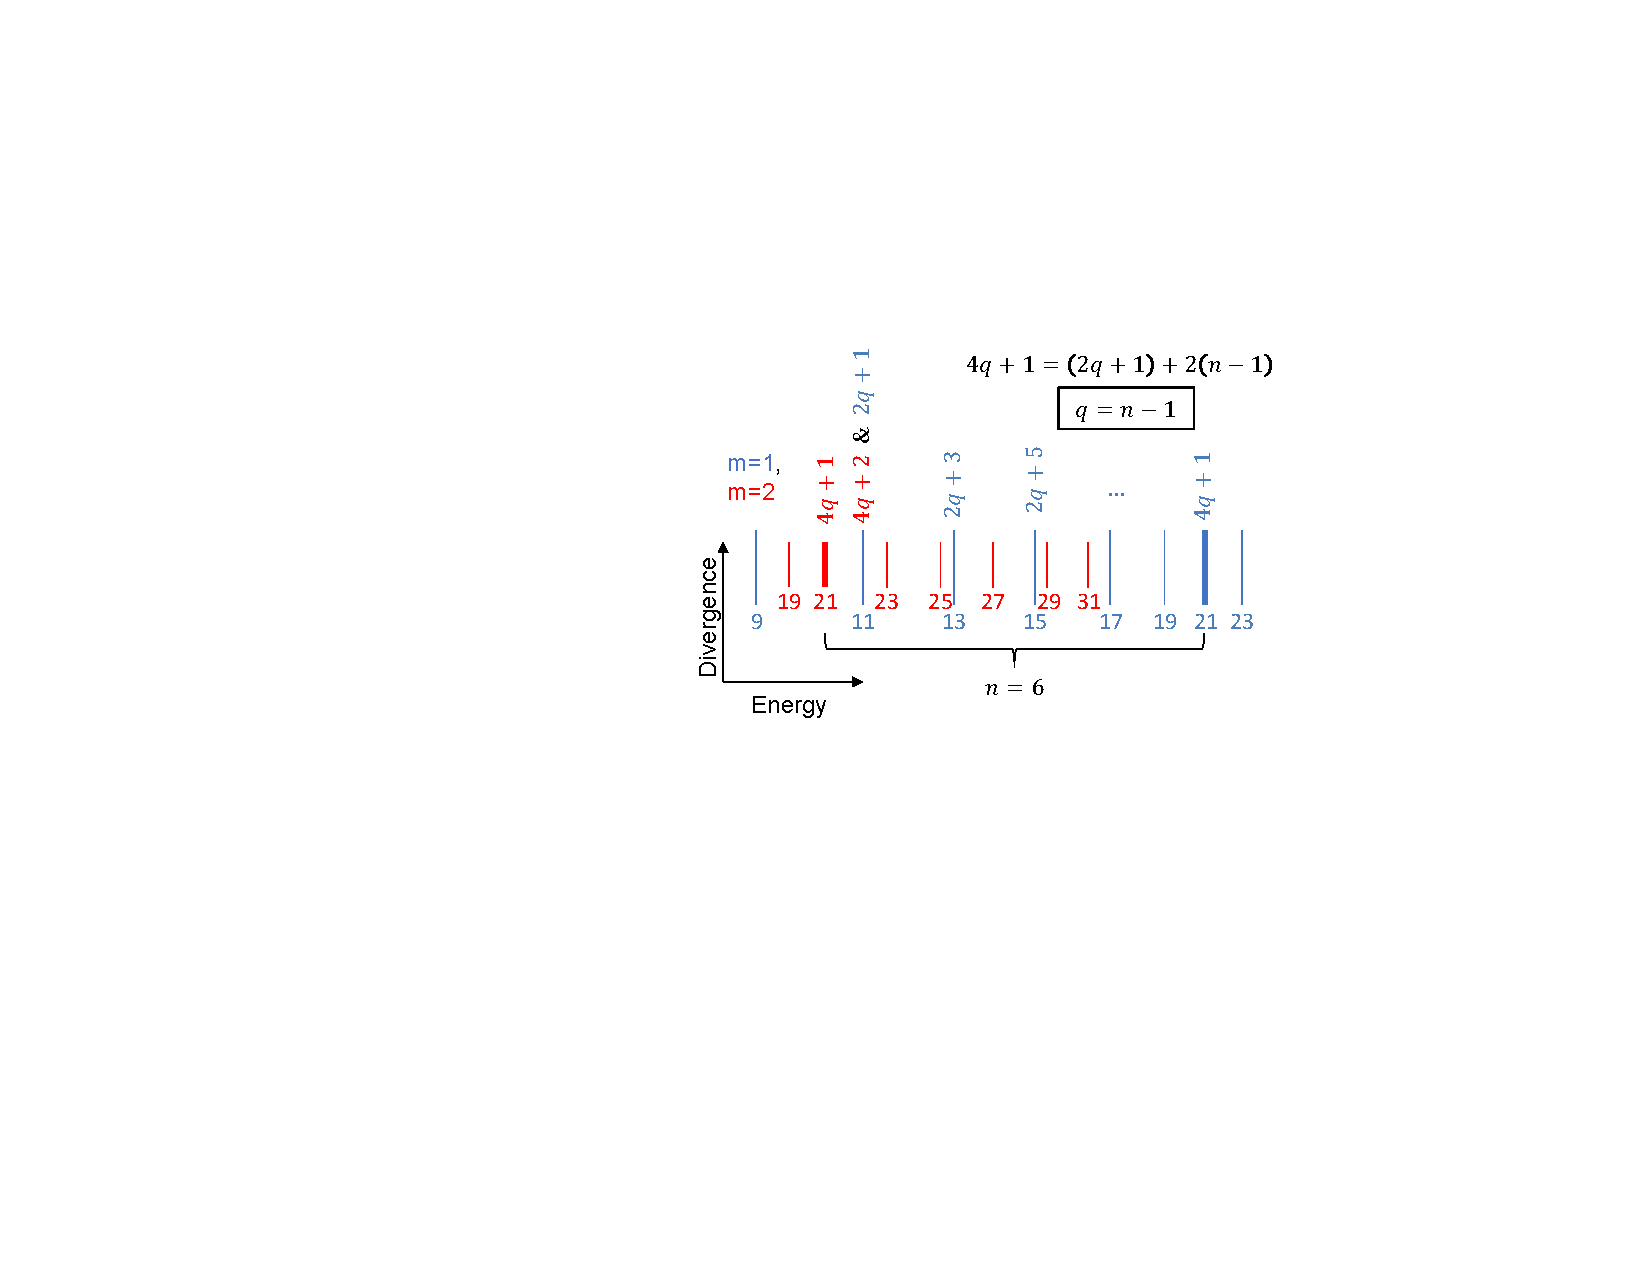
\includegraphics[width=0.75\textwidth]{figures/chap2/harmonic_counting.pdf}
	\caption{Counting scheme to determine the absolute harmonic order.}
	\label{fig:harmonic_counting}
	% chap 2 figures powerpoint.
\end{figure}

\cref{fig:harmonic_counting} schematically shows the effect of having more than an octave of XUV bandwidth is on the detector. The vertical axis is proportional to divergence (unused in this application) and the horizontal axis is proportional to wavelength, with photon energy increasing to the right. The harmonics are denoted as vertical line segments, with \nth{1} order harmonics colored blue and \nth{2} order harmonics colored red. In this cartoon, each harmonic order is labeled with its harmonic order, $i = 11, 13, \dots$, but we have not determined these numbers yet.

If we are able to identify a matched pair of diffraction orders, then we can determine the absolute harmonic order as follows. Let the harmonic order of this matched pair be $i = 4q+1$. This pair is bolded in \cref{fig:harmonic_counting}. If we look at the $m=2$ copy of the $4q+1$ harmonic, there will be an $m=1$ harmonic immediately to the right of it. In $m=2$ space, this position would correspond to $i_{m=2} = 4q+2$, which is even. However we are only creating odd harmonics, so this light must be from an odd diffraction order ($m=1, 3, \dots$). Of the odd diffraction orders, $m=1$ is the brightest, so this harmonic order is $i_{m=1} = (4q+2)/2 = 2q+1$. We now count the number of $m=1$ harmonics harmonics between the matched pair (including the right endpoint), which we will call $n$. In doing so, we are counting the number of $m=1$ harmonics between $i=2q+1$ and $i=4q+1$. We therefore determine $q$ via the following relation:
\begin{equation}
(m=1): 4q+1 = (2q+1) + 2(n-1) \rightarrow q = n - 1
\label{eqn:HO_counting}
\end{equation}
In the cartoon, we count $n=6$ \nth{1} order harmonics (blue line segments) between the bolded matched pair. From \cref{eqn:HO_counting}, we determine that $q = 6 - 1 = 5$, and therefore the matched pair has harmonic order $4q+1 = 21$. Once we know the numerical value of $4q+1$, we can label the remaining harmonics sequentially, as shown in the figure.

At this point, we have a set of $N$ coordinate pairs of spectral pixel and harmonic orders $\{(p_i, HO_i)\}$. We can now fit to a polynomial function and create a functional map between the spectral pixel and the harmonic order, $HO(p)$. If we can identify a single spectral feature located at pixel $p_i$ with a known energy $E_i$, then we can scale the harmonic order function to an energy function: $E(p) = (E_i / HO(p_i)) \times HO(p)$. Usually, the sharp aluminum $L$-edge at 72.3 eV is used for this purpose.

\subsubsection{Two-Source Harmonic Counting Scheme}

\begin{figure}
	\centering
	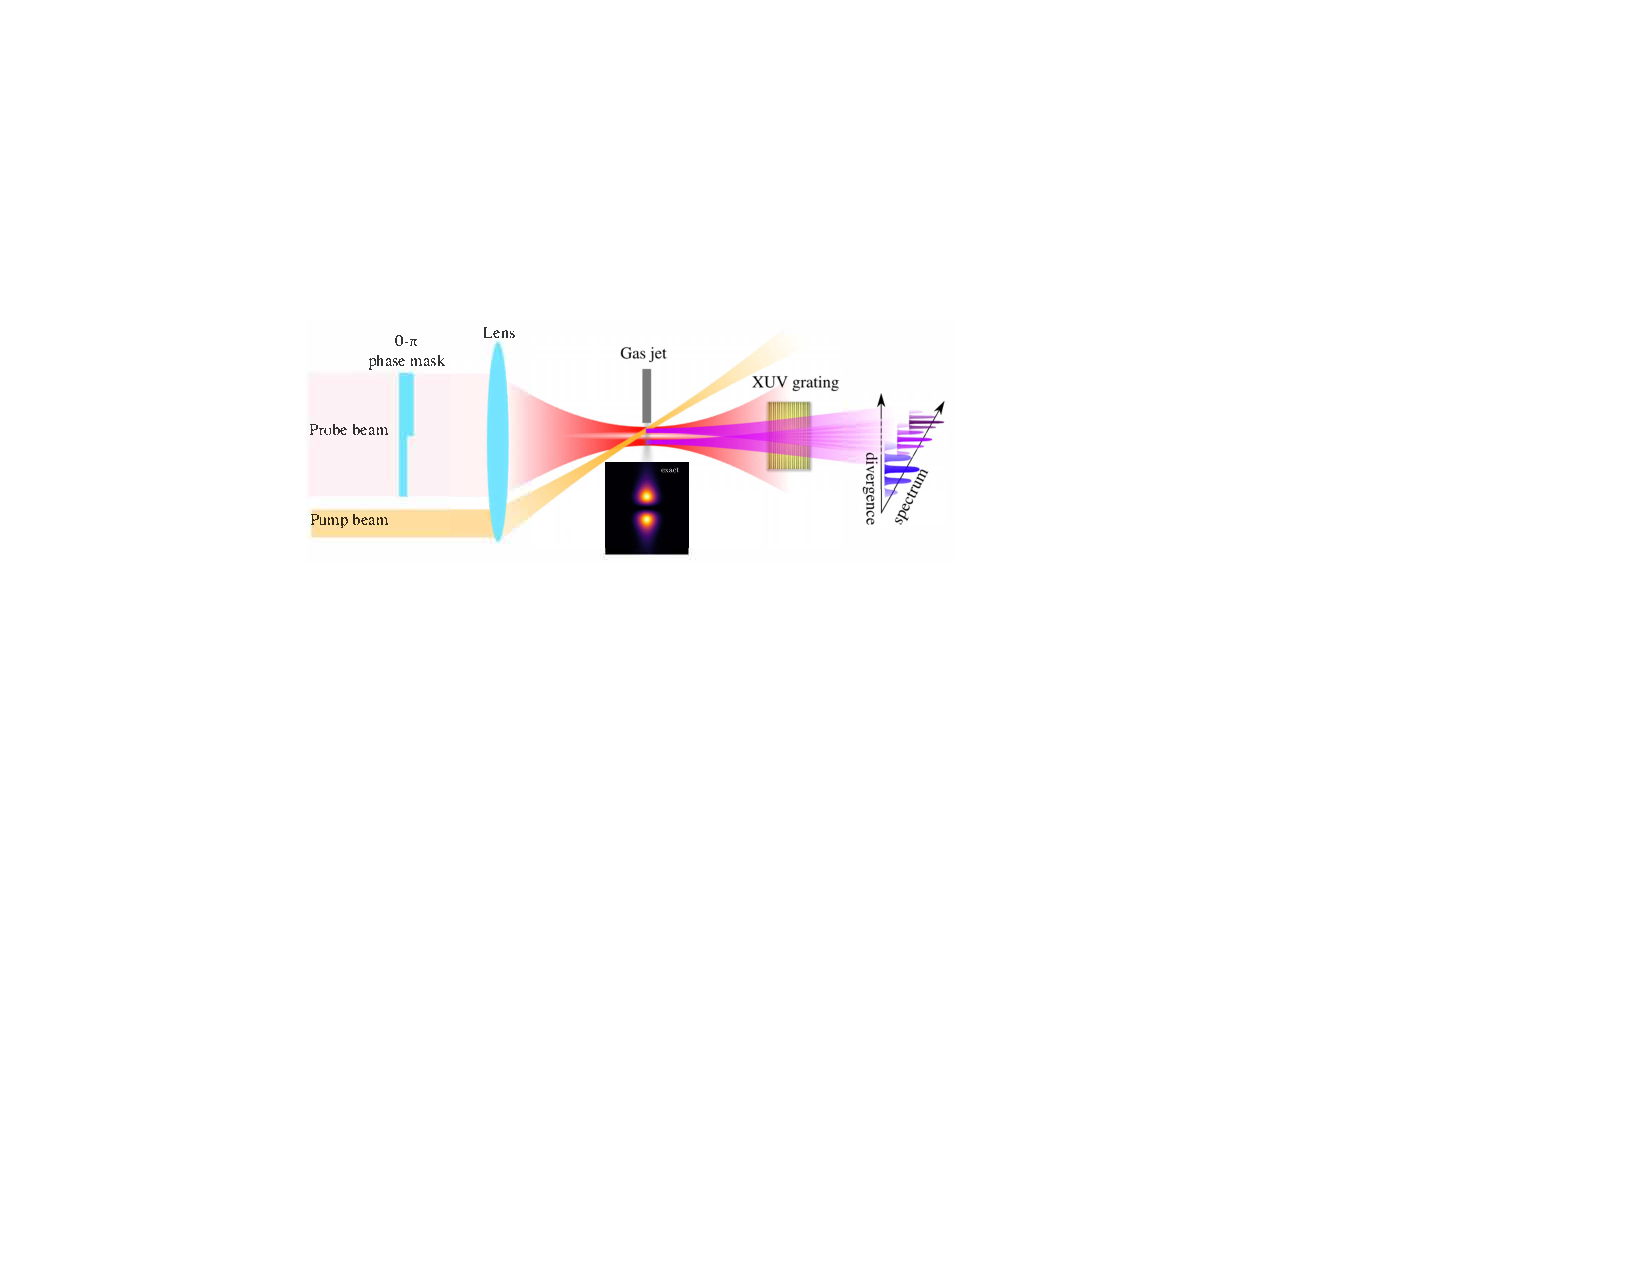
\includegraphics[width=0.75\textwidth]{figures/chap2/two_source_HHG.pdf}
	\caption{Two-source harmonic generation scheme. The pump beam is not used in this application. Extraneous XUV optics are omitted for visual clarity. Figure adapted from \cite{camperTransverseElectromagneticMode2015}.}
	\label{fig:two-source-cartoon}
	% figure copied from camperTransverseElectromagneticMode2015.
\end{figure}

We can use the divergence axis of the spectrometer to identify matching pairs of harmonic orders. We do this by inserting the $\pi$-plate into the laser beam upstream of the generation lens. Recalling the main result of \cref{sec:pi-plate-math}, the $\pi$-plate transforms a TEM\textsubscript{00} beam into a TEM\textsubscript{01}-like beam. The two phase-locked intensity lobes at the focus of the IR beam have a separation $\Delta y_p$:
$$
\Delta y_p \approx \frac{\lambda_1 f}{\sigma}
$$
For $\lambda = 1350 \ \textrm{nm}$, $f=40 \ \textrm{cm}$ and $\sigma = 12.8 \ \textrm{mm}$, the IR spot separation is about 42 $\mu$m. By placing a gas jet at the IR focus, each intensity lobe will locally drive the HHG process. As a result, we will have two spatially separated phase-locked XUV light sources that will interfere in the far field with a spatial frequency $\tilde{k}_q$  \cite{camperTransverseElectromagneticMode2015}:
\begin{equation}
\tilde{k}_q = q \frac{2 \pi a}{\lambda_1 D}
\end{equation}
where $D$ is the source-to-screen distance, $a$ is the distance between the two sources, $\lambda_1$ is the fundamental wavelength, and $q$ is the harmonic order. This setup is schematically shown in \cref{fig:two-source-cartoon}. By performing a Fourier transform along the spatial dimension, we can identify matching pairs ($m=1,2,3,4$) of harmonics. Once we have identified these pairs, we can apply the method described above to find the absolute harmonic order. For more details on two-source harmonic generation, see Stephen Hageman's dissertation \cite{hagemanComplexAttosecondTransientAbsorption2020}.

\begin{figure}
	\centering
	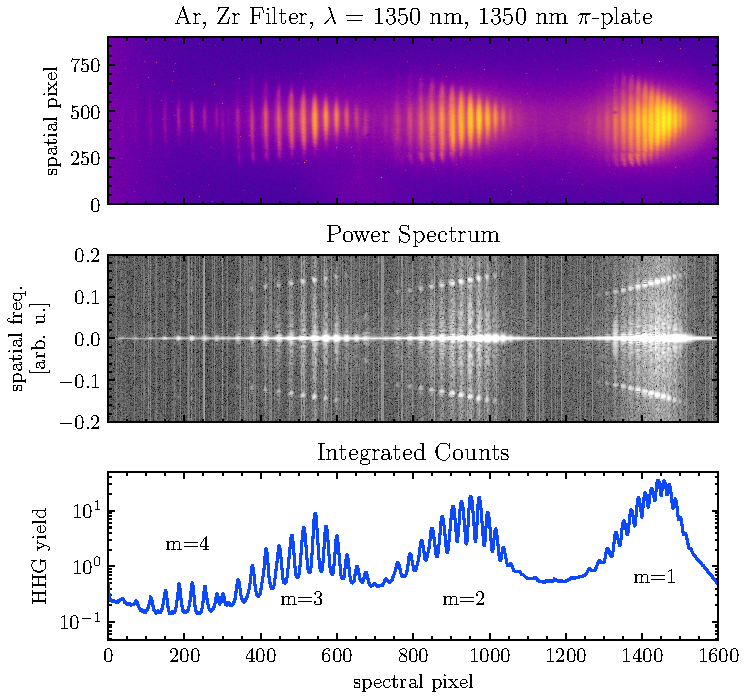
\includegraphics[width=0.9\textwidth]{figures/chap2/multi-order-PiPlate.pdf}
	\caption{Two-source harmonic spectrum. Top panel: log scale 2D detector image. Middle panel: log scale of the power spectrum, computed by taking the FFT of the top panel along spatial dimension. Bottom panel: vertical integration of the top panel.}
	\label{fig:multi-order-PiPlate}
	% figure made in \Python Scripts\Spectrometer\test\2017_09_19.py
\end{figure}

The top panel of \cref{fig:multi-order-PiPlate} shows a harmonic spectrum generated with the 1350 nm $\pi$-plate using argon gas in the low pressure cell (see \cref{sec:LPC}), a fundamental wavelenth of $\lambda=1350 \ \textrm{nm}$, a zirconium filter, and an exposure time of 650 seconds. Along the spectral axis, we see four ``clusters" of harmonics spanning the horizontal axis. We will show below that each ``cluster" corresponds to a different grating diffraction order, with $m=1$ on the right and $m=4$ on the left of the sensor. As $m$ increases, the counts decrease and the dispersion changes, but the clusters are otherwise identical to each other. The finite noise floor of the detector limits our ability to resolve the weakest harmonics. Normally, the $m=3$ and $m=4$ harmonics are too faint to be seen, but they are visible here due to the combination of the Zr filter (which blocks light below 60 eV, see \cref{fig:Filter_transmission_CXRO}) and an abnormally long exposure time. The cutoff energy of this spectrum is approximately 80 eV.

A discrete Fourier transform (FFT) is performed along the spatial dimension of the data shown in the top panel, and the power spectrum is shown in the middle panel of \cref{fig:multi-order-PiPlate}. As discussed above, we expect the spatial frequency of the interference pattern to be proportional to the harmonic energy, and this is exactly what we see. Within a given diffraction order, the spatial frequency increases as the harmonic number increases. Across the harmonic clusters, we see the same increase of spatial frequency with respect to increasing harmonic order, which confirms our hypothesis that each harmonic cluster corresponds to a unique grating diffraction order.

The bottom panel of \cref{fig:multi-order-PiPlate} shows the spatial integration of the detector image. We can see that the efficiency of the grating decreases with increasing $m$, and only a few $m=4$ harmonics are visible.

\begin{figure}
	\centering
	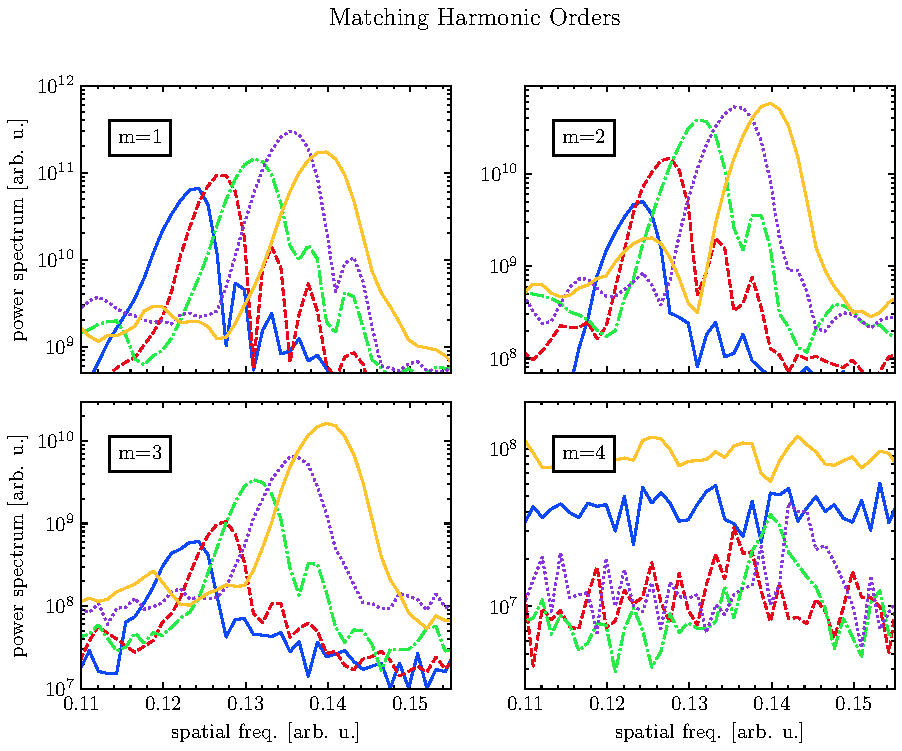
\includegraphics[width=0.9\textwidth]{figures/chap2/twosource-matching-HO.pdf}
	\caption{Integrated power spectrum (middle panel of \cref{fig:multi-order-PiPlate}) for selected harmonic orders and different diffraction orders. Harmonics with the matching spatial frequencies share the same line style and color.}
	\label{fig:twosource-matching-HO}
	% figure made in \Python Scripts\Spectrometer\test\2017_09_19.py
\end{figure}

Any two harmonic orders with the same dominant spatial frequency must have the same wavelength and therefore must be the same harmonic order. We can use this fact to match harmonic orders across the different diffraction orders. \cref{fig:twosource-matching-HO} shows the power spectrum, integrated around the width of each harmonic, for seven matching harmonics orders. The $m=4$ harmonic signal is too weak to resolve most of the spatial frequencies, except for two harmonics.

Now that we have identified matching harmonics, we can calculate the relative grating efficiency, but we must take care in doing so. First, the spectral dispersion is different for each diffraction order, so the height of the harmonic is not a valid metric -- we must use the integrated harmonic yield\footnote{Note that for this calculation, there is no need to include the Jacobian or convert the spectral axis to the energy basis, as the following quantity is conserved: $\int f_p(p) \dd{p} = \int f_E(E) \dd{E}$. See the later section on the Jacobian for more details.}. Secondly, only a few $m=4$ diffraction orders are visible, so we should take care to integrate over the same spectral region for each diffraction order. Finally, the harmonics overlap each other, and we can see the amount of overlap varies for each diffraction order -- so we can't just numerically sum the signal over a discrete number of harmonics. We get around this problem by fitting the harmonic spectrum to a sum of Gaussians and using the fitted values to analytically integrate the contribution of a subset of common harmonics.

\begin{figure}
	\centering
	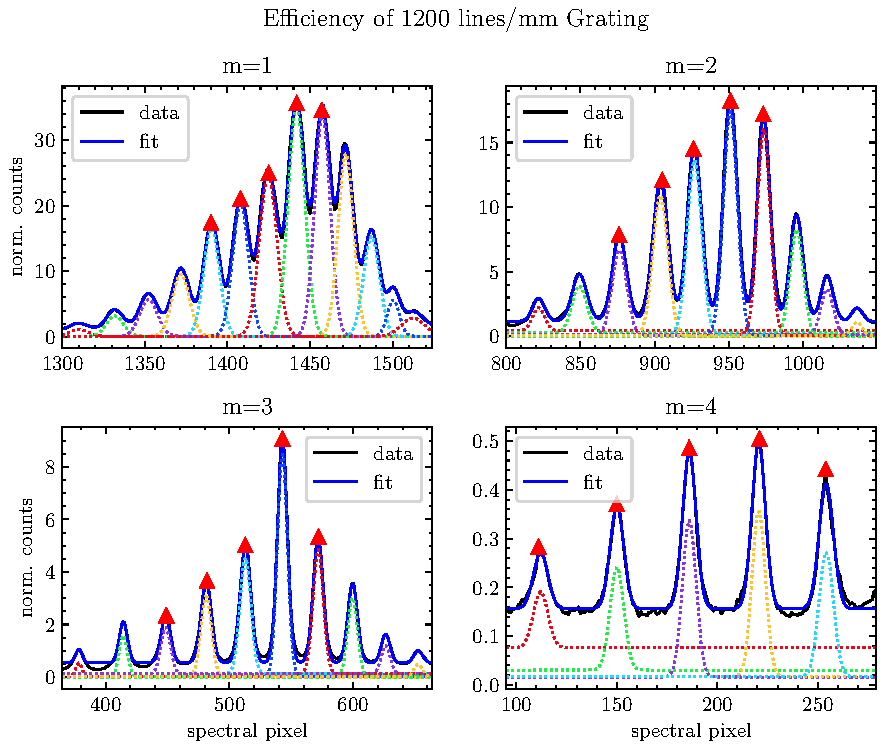
\includegraphics[width=0.9\textwidth]{figures/chap2/grating-efficiency.pdf}
	\caption{Gaussian fit to the spectrum in \cref{fig:multi-order-PiPlate}. Triangles indicate the harmonics used in the grating efficiency calculation; matching colors indicate matching harmonic order, following \cref{fig:twosource-matching-HO}.}
	\label{fig:grating-efficiency}
	% figure made in \Python Scripts\Spectrometer\test\2017_09_19.py
\end{figure}

This analysis is shown in \cref{fig:grating-efficiency}. For each diffraction order, we fit the spectra to a series of Gaussians (dashed lines, each of the form ${y_i = a_i \exp \left[ (x-b_i)^2 / (2 c_i^2) \right] + d_i}$). The matching harmonics, identified in \cref{fig:twosource-matching-HO}, are indicated with red triangles. For each diffraction order, we integrate the total yield of the tagged harmonics via ${\eta_i = \Sigma_i \sqrt{2 \pi} a_i |c_i|}$. Next, we calculate the grating efficiency (relative to the $m=1$ diffraction). The result is:
\begin{align*}
\frac{\eta_2}{\eta_1} &= 42.2 \% \\
\frac{\eta_3}{\eta_1} &= 13.0 \% \\
\frac{\eta_4}{\eta_1} &= 0.6 \%
\end{align*}
If we neglect the zero-order diffraction and the contributions of higher order terms (${1 = \Sigma_{i=1}^4 \eta_i}$), then we can calculate the absolute diffraction efficiency of the grating:
\begin{align*}
\eta_1 \simeq  64.2 \% \\
\eta_2 \simeq 27.1 \% \\
\eta_3 \simeq 8.4 \% \\
\eta_4 \simeq 0.4 \%
\end{align*}
These grating efficiencies are consistent with the values found in the manufacturer's specification sheet.


\subsubsection{Argon Fano Resonances}

The spectrometer can also be calibrated over a limited spectral range using a collection of known spectral features. The Fano resonance, which is due to an interference between bound and continuum states, can be used for this purpose. The Fano cross section $\sigma$ is parameterized by \cite{sorensenArgon3sAutoionization1994,caretteMulticonfigurationalHartreeFockClosecoupling2013}:
\begin{equation}
\sigma = \frac{(q+\epsilon)^2}{1+\epsilon^2} \sigma_a + \sigma_b
\label{eqn:Fano_sigma}
\end{equation}
where $\sigma_a$ is the amplitude of the resonance, $\sigma_b$ is the slowly varying background scattering, $q$ is the asymmetry parameter and $\epsilon$ is the normalized distance from the resonance, defined as:
\begin{equation}
\epsilon \equiv \frac{\hbar \omega - E_r}{\Gamma/2}
\end{equation}
where $\hbar \omega$ is the photon energy, $E_r$ is the resonance energy and $\Gamma$ is the width. Taking the derivative, we find that the cross section $\sigma$ has extrema at the following photon energies:
\begin{align}
\hbar \omega^+ &= E_r + \frac{\Gamma}{2 q} \\
\hbar \omega^- &= E_r - \frac{q \Gamma}{2}
\end{align}

\begin{figure}
	\centering
	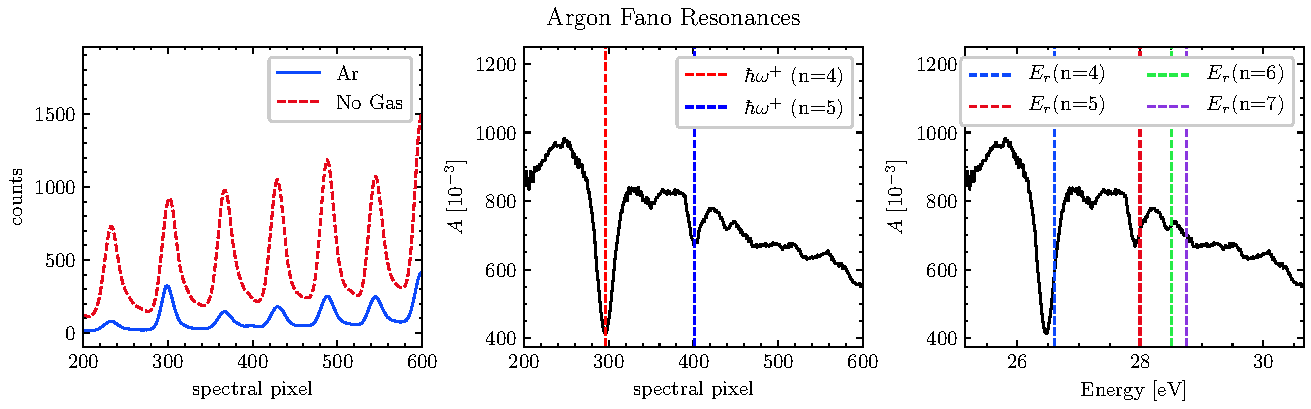
\includegraphics[width=1.0\textwidth]{figures/chap2/ar-fano-calibration.pdf}
	\caption{Fano resonances used for low energy spectral calibration. Left panel: XUV spectra with and without argon gas at the XUV focus. Middle panel: measured absorbance $A$ of argon showing the absorption profile of the $n=4$ and $n=5$ $3s3p^6np$ resonances. Right panel: calibrated spectra showing the expected locations the higher resonances.}
	\label{fig:fano-calibration}
	% figure made in \Python Scripts\Spectrometer\test\2019_09_19_fano.py
\end{figure}

In argon, the $3s3p^6np$ Fano resonance series occurs between 26.6 and 29 eV. We can observe the Fano cross section in argon by recording XUV spectra with and without gas at the XUV focus, as shown in the left panel of \cref{fig:fano-calibration}. A low pressure cell located at the XUV focus delivers the gas in the target chamber (see \cref{sec:LPC}). The middle panel shows the absorption $A$ of the gas sample, defined as the logarithm of the ratio of the collected spectra $S$:
\begin{equation}
A = - \log_{10} \left( \frac{S_{\textrm{Ar}}}{S_{\textrm{No gas}}} \right)
\end{equation}

\begin{table}[]
	\centering
	\begin{tabular}{c|c|c|c}
		n & $E_r$ {[}eV{]} & $\Gamma$ {[}meV{]} & q \\ \hline
		4 & 26.605 & 80.2 & -0.286 \\ \hline
		5 & 27.994 & 28.5 & -0.177 \\ \hline
		6 & 28.509 & 12.2 & -0.135 \\ \hline
		7 & 28.757 & 4.5 & -0.125
	\end{tabular}
	\caption{Experimentally measured Fano parameters for the $3s3p^6np$ resonance series in argon \cite{caretteMulticonfigurationalHartreeFockClosecoupling2013}.}
	\label{tab:fano-parameters}
\end{table}

Overall, we see a broad absorption with prominent emission peaks ($\hbar \omega^+$), corresponding to the $n=4,5$ resonances in the $3s3p^6np$ series. The location of these peaks is used to calibrate the spectrometer in the low photon energy region using the literature values of the Fano profile (see \cref{tab:fano-parameters}). The right panel shows the calibrated Fano absorption spectra and highlights the expected locations of the higher resonances.


\subsubsection{The Jacobian}
\label{sec:jacobian}

Once we have the calibration function, we need to scale the measured signal by the Jacobian in order to conserve energy \cite{mooneyGetBasicsRight2013}. Let $f_p(p)$ be the function that represents the measured XUV counts at spectral pixel $p$:
\begin{equation}
f_p(p): \textrm{ spectral pixel} \rightarrow \textrm{counts}
\end{equation}
During the calibration step, we convert the spectral pixel axis to energy [eV] using a function $E(p)$, usually a polynomial:
\begin{align}
E(p)&: \textrm{ spectral pixel} \rightarrow \textrm{energy [eV]} \\
E(p) &= a_0 + a_1 p + a_2 p^2 + a_3 p^3 + a_4 p^4 + ...
\end{align}
Likewise, we define the inverse of $E(p)$ to be:
\begin{align}
p(E)&: \textrm{ energy [eV]} \rightarrow \textrm{spectral pixel} \\
p(E) &\equiv E^{-1}(p)
\end{align}
We want calculate the XUV counts in the energy basis. That is, we want to convert $f_p(p)$ to $f_E(E)$ using the Jacobian. By conservation of energy, we have the relation:
\begin{equation}
f_p (p) \dd{p} = f_E (E) \dd{E}
\end{equation}
Rearangement of the above equation leads us to the desired result:
\begin{equation}
f_E (E) = f_p (p) \dv{p}{E} = f_p (p) \dv{E} p(E)
\end{equation}

\section{Conclusion}

In this chapter, we described the laser system, including the active pointing correction system, the external compressor and TOPAS. The pulse duration was characterized using the FROG technique and the interaction pulse duration was estimated to be 63.7 fs. Next, the home-built vacuum system was described. Different XUV refocusing optics were discussed within the goal of maximizing reflectivity and minimizing abberations at the focus. The aberrations of two candidate mirror geometries were analyzed, and it was found that an ellipsoidal mirror was superior to a toroidal mirror when used in a demagnifying configuration. The IR optics were described and numerically modeled, and we obtained an intensity profile at the sample focal plane that will be used in \cref{chap:ATAS_in_Ge} to model the laser-sample interaction. Finally, the XUV spectrometer was described and methods to spectrally calibrate it were developed.